
\documentclass[a4paper, 12pt]{book}

\usepackage[utf8x]{inputenc}   % omogoča uporabo slovenskih črk kodiranih v formatu UTF-8
\usepackage[slovene,english]{babel}    % naloži, med drugim, slovenske delilne vzorce
\usepackage{titlesec}
\usepackage[pdftex]{graphicx}  % omogoča vlaganje slik različnih formatov
\usepackage{fancyhdr}          % poskrbi, na primer, za glave strani
\usepackage{amssymb}           % dodatni simboli
\usepackage{amsmath}           % eqref, npr.
%\usepackage{hyperxmp}
\usepackage{amsthm}
\usepackage[pdftex, colorlinks=true,
						citecolor=black, filecolor=black, 
						linkcolor=black, urlcolor=black,
						pagebackref=false, 
						pdfproducer={LaTeX}, pdfcreator={LaTeX}, hidelinks]{hyperref}
\usepackage[export]{adjustbox}
\usepackage{float}
\usepackage[table,xcdraw]{xcolor}
% for writing code
\usepackage{listings}
\usepackage{color}

\definecolor{dkgreen}{rgb}{0,0.6,0}
\definecolor{gray}{rgb}{0.5,0.5,0.5}
\definecolor{mauve}{rgb}{0.58,0,0.82}

\lstset{frame=tb,
  language=Java,
  aboveskip=3mm,
  belowskip=3mm,
  showstringspaces=false,
  columns=flexible,
  basicstyle={\small\ttfamily},
  numbers=none,
  numberstyle=\tiny\color{gray},
  keywordstyle=\color{blue},
  commentstyle=\color{dkgreen},
  stringstyle=\color{mauve},
  breaklines=true,
  breakatwhitespace=true,
  tabsize=3
}
%%%%%%%%%%%%%%%%%%%%%%%%%%%%%%%%%%%%%%%%
%	DIPLOMA INFO
%%%%%%%%%%%%%%%%%%%%%%%%%%%%%%%%%%%%%%%%
\newcommand{\ttitle}{Aplikacija za gamifikacijo mobilnega učenja}
\newcommand{\ttitleEn}{Gamified mobile learning application}
\newcommand{\tsubject}{\ttitle}
\newcommand{\tsubjectEn}{\ttitleEn}
\newcommand{\tauthor}{Simon Špehar}
\newcommand{\tkeywords}{mobilno učenje, gamifikacija, mobilna aplikacija, spletna aplikacija, PHP, Javascript, Laravel, Ionic, REST}
\newcommand{\tkeywordsEn}{mobile learning, gamification, mobile application, web application, PHP, Javascript, Laravel, Ionic, REST}



\usepackage{hyperref}
%%%%%%%%%%%%%%%%%%%%%%%%%%%%%%%%%%%%%%%%
%	HYPERREF SETUP
%%%%%%%%%%%%%%%%%%%%%%%%%%%%%%%%%%%%%%%%
\hypersetup{pdftitle={\ttitle}}
\hypersetup{pdfsubject=\ttitleEn}
\hypersetup{pdfauthor={\tauthor, ss5781@student.uni-lj.si}}
\hypersetup{pdfkeywords=\tkeywordsEn}


 


%%%%%%%%%%%%%%%%%%%%%%%%%%%%%%%%%%%%%%%%
% postavitev strani
%%%%%%%%%%%%%%%%%%%%%%%%%%%%%%%%%%%%%%%%  

\addtolength{\marginparwidth}{-20pt} % robovi za tisk
\addtolength{\oddsidemargin}{40pt}
\addtolength{\evensidemargin}{-40pt}

\renewcommand{\baselinestretch}{1.3} % ustrezen razmik med vrsticami
\setlength{\headheight}{15pt}        % potreben prostor na vrhu
\renewcommand{\chaptermark}[1]%
{\markboth{\MakeUppercase{\thechapter.\ #1}}{}} \renewcommand{\sectionmark}[1]%
{\markright{\MakeUppercase{\thesection.\ #1}}} \renewcommand{\headrulewidth}{0.5pt} \renewcommand{\footrulewidth}{0pt}
\fancyhf{}
\fancyhead[LE,RO]{\sl \thepage} \fancyhead[LO]{\sl \rightmark} \fancyhead[RE]{\sl \leftmark}



\newcommand{\BibTeX}{{\sc Bib}\TeX}

%%%%%%%%%%%%%%%%%%%%%%%%%%%%%%%%%%%%%%%%
% naslovi
%%%%%%%%%%%%%%%%%%%%%%%%%%%%%%%%%%%%%%%%  


\newcommand{\autfont}{\Large}
\newcommand{\titfont}{\LARGE\bf}
\newcommand{\clearemptydoublepage}{\newpage{\pagestyle{empty}\cleardoublepage}}
\setcounter{tocdepth}{1}	      % globina kazala

%%%%%%%%%%%%%%%%%%%%%%%%%%%%%%%%%%%%%%%%
% konstrukti
%%%%%%%%%%%%%%%%%%%%%%%%%%%%%%%%%%%%%%%%  
\newtheorem{izrek}{Izrek}[chapter]
\newtheorem*{definition*}{Definicija}

\newenvironment{dokaz}{\emph{Dokaz.}\ }{\hspace{\fill}{$\Box$}}

%%%%%%%%%%%%%%%%%%%%%%%%%%%%%%%%%%%%%%%%%%%%%%%%%%%%%%%%%%%%%%%%%%%%%%%%%%%%%%%
%% PDF-A
%%%%%%%%%%%%%%%%%%%%%%%%%%%%%%%%%%%%%%%%%%%%%%%%%%%%%%%%%%%%%%%%%%%%%%%%%%%%%%%

%%%%%%%%%%%%%%%%%%%%%%%%%%%%%%%%%%%%%%%% 
% define medatata
%%%%%%%%%%%%%%%%%%%%%%%%%%%%%%%%%%%%%%%% 
\def\Title{\ttitle}
\def\Author{\tauthor, ss5781@student.uni-lj.si}
\def\Subject{\ttitleEn}
\def\Keywords{\tkeywordsEn}

%%%%%%%%%%%%%%%%%%%%%%%%%%%%%%%%%%%%%%%% 
% \convertDate converts D:20080419103507+02'00' to 2008-04-19T10:35:07+02:00
%%%%%%%%%%%%%%%%%%%%%%%%%%%%%%%%%%%%%%%% 
\def\convertDate{%
    \getYear
}

{\catcode`\D=12
 \gdef\getYear D:#1#2#3#4{\edef\xYear{#1#2#3#4}\getMonth}
}
\def\getMonth#1#2{\edef\xMonth{#1#2}\getDay}
\def\getDay#1#2{\edef\xDay{#1#2}\getHour}
\def\getHour#1#2{\edef\xHour{#1#2}\getMin}
\def\getMin#1#2{\edef\xMin{#1#2}\getSec}
\def\getSec#1#2{\edef\xSec{#1#2}\getTZh}
\def\getTZh +#1#2{\edef\xTZh{#1#2}\getTZm}
\def\getTZm '#1#2'{%
    \edef\xTZm{#1#2}%
    \edef\convDate{\xYear-\xMonth-\xDay T\xHour:\xMin:\xSec+\xTZh:\xTZm}%
}

\expandafter\convertDate\pdfcreationdate 

%%%%%%%%%%%%%%%%%%%%%%%%%%%%%%%%%%%%%%%%
% get pdftex version string
%%%%%%%%%%%%%%%%%%%%%%%%%%%%%%%%%%%%%%%% 
\newcount\countA
\countA=\pdftexversion
\advance \countA by -100
\def\pdftexVersionStr{pdfTeX-1.\the\countA.\pdftexrevision}


%%%%%%%%%%%%%%%%%%%%%%%%%%%%%%%%%%%%%%%%
% XMP data
%%%%%%%%%%%%%%%%%%%%%%%%%%%%%%%%%%%%%%%%  
\usepackage{xmpincl}
\includexmp{pdfa-1b}

%%%%%%%%%%%%%%%%%%%%%%%%%%%%%%%%%%%%%%%%
% pdfInfo
%%%%%%%%%%%%%%%%%%%%%%%%%%%%%%%%%%%%%%%%  
\pdfinfo{%
    /Title    (\ttitle)
    /Author   (\tauthor)
    /Subject  (\ttitleEn)
    /Keywords (\tkeywordsEn)
    /ModDate  (\pdfcreationdate)
    /Trapped  /False
}


%%%%%%%%%%%%%%%%%%%%%%%%%%%%%%%%%%%%%%%%%%%%%%%%%%%%%%%%%%%%%%%%%%%%%%%%%%%%%%%
%%%%%%%%%%%%%%%%%%%%%%%%%%%%%%%%%%%%%%%%%%%%%%%%%%%%%%%%%%%%%%%%%%%%%%%%%%%%%%%

\begin{document}
\selectlanguage{slovene}
\frontmatter
\setcounter{page}{1} %
\renewcommand{\thepage}{}       % preprecimo težave s številkami strani v kazalu

%%%%%%%%%%%%%%%%%%%%%%%%%%%%%%%%%%%%%%%%
%naslovnica
 \thispagestyle{empty}%
   \begin{center}
    {\large\sc Univerza v Ljubljani\\%
      Fakulteta za računalništvo in informatiko}%
    \vskip 10em%
    {\autfont \tauthor\par}%
    {\titfont \ttitle \par}%
    {\vskip 2em \textsc{DIPLOMSKO DELO\\[2mm]
    VISOKOŠOLSKI STROKOVNI ŠTUDIJSKI PROGRAM PRVE STOPNJE RAČUNALNIŠTVO IN INFORMATIKA}\par}%
    \vfill\null%
    {\large \textsc{Mentor}: viš.\ pred.\ dr.  Aljaž Zrnec\par}%
    {\vskip 2em \large Ljubljana, 2017 \par}%
\end{center}
% prazna stran
\clearemptydoublepage

%%%%%%%%%%%%%%%%%%%%%%%%%%%%%%%%%%%%%%%%
%copyright stran
\thispagestyle{empty}
\vspace*{8cm}

\noindent
{\sc Copyright}. 
Rezultati diplomske naloge so intelektualna lastnina avtorja in Fakultete za računalništvo in informatiko Univerze v Ljubljani.
Za objavo in koriščenje rezultatov diplomske naloge je potrebno pisno privoljenje avtorja, Fakultete za računalništvo in informatiko ter mentorja.
\begin{center}
\mbox{}\vfill
\emph{Besedilo je oblikovano z urejevalnikom besedil \LaTeX.}
\end{center}
% prazna stran
\clearemptydoublepage

%%%%%%%%%%%%%%%%%%%%%%%%%%%%%%%%%%%%%%%%
% stran 3 med uvodnimi listi
\thispagestyle{empty}
\vspace*{4cm}

\noindent
Fakulteta za računalništvo in informatiko izdaja naslednjo nalogo:
\medskip
\begin{tabbing}
\hspace{32mm}\= \hspace{6cm} \= \kill




Tematika naloge: Aplikacija za gamifikacijo mobilnega učenja
\end{tabbing}
V zadnjih letih se pojavlja na trgu vedno več aplikacij, pri katerih zasledimo elemente iger, čeprav je njihova primarna funkcija namenjena nečemu drugemu kot samo zabavi. To so aplikacije, ki uporabljajo t.i. principe gamifikacije. V okviru diplomske naloge raziščite, kaj bi lahko na mobilni napravi uporabili, da bi gamificirali proces mobilnega učenja. Pri tem poskusite vključiti senzorje, ki so na voljo na napravah, da izboljšate uporabniško izkušnjo. Izdelajte mobilno aplikacijo, ki uporablja proces gamifikacije za potrebe mobilnega učenja.
\vspace{15mm}



\vspace{2cm}

% prazna stran
\clearemptydoublepage

% zahvala
\thispagestyle{empty}\mbox{}\vfill\null\it%
Zahvaljujem se mentorju viš.\ pred.\ dr.  Aljažu Zrnecu za strokovno pomoč pri izdelavi diplomske naloge ter družini in prijateljem za vzpodbudne besede med študijem.
\rm\normalfont

% prazna stran
\clearemptydoublepage

%%%%%%%%%%%%%%%%%%%%%%%%%%%%%%%%%%%%%%%%
% posvetilo
%\thispagestyle{empty}\mbox{}{\vskip0.20\textheight}\mbox{}\hfill%\begin{minipage}{0.55\textwidth}%
%Svoji dragi Alenčici.
%\normalfont\end{minipage}

% prazna stran
\clearemptydoublepage

%%%%%%%%%%%%%%%%%%%%%%%%%%%%%%%%%%%%%%%%
% kazalo
\pagestyle{empty}
\def\thepage{}% preprecimo tezave s stevilkami strani v kazalu
\tableofcontents{}


% prazna stran
\clearemptydoublepage

%%%%%%%%%%%%%%%%%%%%%%%%%%%%%%%%%%%%%%%%
% seznam kratic

\chapter*{Seznam uporabljenih kratic}

\begin{tabular}{l|l|l}
  {\bf kratica} & {\bf angleško} & {\bf slovensko} \\ \hline
  % after \\: \hline or \cline{col1-col2} \cline{col3-col4} ...
   {\bf OS} & Operating system & Operacijski sistem \\
   {\bf GPS} & Global positioning system & Globalni sistem pozicioniranja \\
   {\bf BLE} & Bluetooth low energy & Bluetooth nizkih energij \\
   {\bf ORM} & Object-relational mapping & Objektno relacijsko preslikovanje \\
   {\bf JSON} & JavaScript Object Notation & Objektni JavaScript zapis \\
   {\bf API} & Application Programming Interface & Aplikacijski programski vmesnik \\  
   {\bf URL} & Uniform resource locator & Enolični krajevnik vira \\
   {\bf HTML} & Hypertext Transfer Protocol & Protokol za prenos hiperteksta \\
   {\bf CLI} & Command line interface & Ukazna vrstica \\
   {\bf TTS} & Text to speech & Tekst v govor \\
   {\bf STT} & Speech to text & Govor v tekst \\
   {\bf SQL} & Structured Query Language & Strukturirani poizvedovalni jezik\\
   {\bf QR} & Quick response & Hiter odziv \\
   
\end{tabular}



% prazna stran
\clearemptydoublepage

%%%%%%%%%%%%%%%%%%%%%%%%%%%%%%%%%%%%%%%%
% povzetek
\addcontentsline{toc}{chapter}{Povzetek}
\chapter*{Povzetek}

\noindent\textbf{Naslov:} Aplikacija za gamifikacijo mobilnega učenja
\bigskip

\noindent Mobilno učenje je nekaj s čimer se dandanes, namensko ali nenamensko, sreča večina ljudi pri uporabi mobilnih naprav. Za kaj pravzaprav gre, oziroma kaj predstavlja mobilno učenje, predstavimo v prvem delu diplomske naloge, kjer se vrnemo na začetke mobilnega učenja, ter razložimo pogoje za mobilno učenje. Predstavimo tudi različne načine dostopa do mobilnih učnih vsebin.\\Motivacija pri uporabi takšnega učenja ima pomembno vlogo, saj želimo ponuditi uporabniško izkušnjo, s katero uporabnika prepričamo, da aplikacijo uporabi večkrat in, da ta zanj ostane zanimiva. Slednji problem rešuje t.i. gamifikacija. V nadaljevanju opišemo elemente gamifikacije in s primerom pokažemo kako jih lahko vključimo v naš sistem. Opisali bomo funkcije mobilnih naprav, ki jih lahko izkoristimo za še boljšo uporabniško izkušnjo v naši aplikaciji.\\V drugem delu diplomske naloge se posvetimo izdelavi aplikacije za mobilno učenje, ki uporablja elemente gamifikacije. Razložili bomo proces razvoja takšnega sistema, katere tehnologije smo uporabili ter prikazali delovanje mobilne in spletne aplikacije.
%\noindent\textbf{Povzetek:} 

\bigskip

\noindent\textbf{Ključne besede:} \tkeywords.
% prazna stran
\clearemptydoublepage

%%%%%%%%%%%%%%%%%%%%%%%%%%%%%%%%%%%%%%%%
% abstract
\selectlanguage{english}
\addcontentsline{toc}{chapter}{Abstract}
\chapter*{Abstract}

\noindent\textbf{Title:} Gamified mobile learning application
\bigskip

%\noindent\textbf{Abstract:} 
\noindent Mobile learning is something that most people today use when using mobile devices, whether intentionally or unintentionally. In the first part of the thesis, we return to the beginnings of mobile learning and present what mobile learning actually is. We also present various ways of accessing mobile learning content.\\Motivation in mobile learning activities plays an important role, since we want to keep it interesting for the users so they don't stop using it. The latter problem solves the so-called gamification. We continue describing the elements of gamification and, by way of example, show how we can integrate them into our system. We will describe the features of mobile devices that can be utilized for an even better user experience in our application.\\The second part of thesis is devoted to the development of a mobile learning application that uses elements of gamification. We will explain the development process of such a system, which technologies we have used and the operation of mobile and web application.
\bigskip

\noindent\textbf{Keywords:} \tkeywordsEn.
\selectlanguage{slovene}
% prazna stran
\clearemptydoublepage

%%%%%%%%%%%%%%%%%%%%%%%%%%%%%%%%%%%%%%%%
\mainmatter
\setcounter{page}{1}
\pagestyle{fancy}

\chapter{Uvod}
\label{ch1}
Mobilne tehnologije dosegajo vedno večje razsežnosti in danes omogočajo veliko možnosti za povezovanje, sodelovanje in komunikacijo med uporabniki. Mobilne naprave, ki takšne tehnologije podpirajo, postajajo vse boljše. Postale so del našega življenja pri vsakdanjih opravilih, poslovnih procesih, zabavi in izobraževanju. Mobilno učenje postaja vse bolj priljubljeno, saj so vsebine prilagojene uporabnikom in pri dostopu nismo časovno ali prostorsko omejeni. Figurativno lahko rečemo, da je svet postal učilnica.

Hiter razvoj pa nima samo pozitivnega učinka na uporabnike mobilnih naprav. Če aplikacija ni dovolj zanimiva za uporabnika, bo ta hitro izgubil interes in svoj čas, ki ga preživi na mobilni napravi posvetil nečemu drugemu, naprimer igram. Igre so najbolj priljubljen način preživljanja prostega časa, bodisi v realnem ali pa v virtualnem svetu. Nekaj časa nazaj se je pojavila ideja, da bi začeli v aplikacije, ki primarno niso namenjene zabavi, vključevati elemente, ki se pojavljajo v igrah. Nastal je pojem gamifikacija.\\ V diplomskem delu smo raziskali kaj je in kaj ni mobilno učenje, kaj je gamifikacija, kaj so njeni elementi in prednosti, kako jo implementirati pri mobilnem učenju in na kakšne načine lahko izkoristimo funkcije, ki nam jih ponujajo mobilne naprave, za potrebe gamifikacije mobilnega učenja. 

Ustvarili smo gamificirano aplikacijo za mobilno učenje, ki omogoča učenje različnih vsebin glede na lokacijo naprave. Sestavljena je iz dveh delov. Spletne aplikacije za dodajanje vsebine, ter mobilne aplikacije namenjene učenju. Uporabili smo več elementov gamifikacije, ki jih bomo v kasnejših poglavjih predstavili. Uporabniki bodo zbirali točke z obiskovanjem krajev kjer se predmeti učenja nahajajo, tako bo učenje postavljeno v kontekst z lokacijo. Uporabniki bodo zbirali točke tudi z odgovarjanjem na različna vprašanja, sorodna z obiskano lokacijo oziroma predmetom učenja. Uporabnik z zbiranjem točk prehaja med različnimi težavnostnimi nivoji, ki prinašajo več različnih in mogoče težjih izzivov.\\Vsebino želimo ohraniti kratko in jedrnato, zato bomo omejili količino informacij, ki jih uporabnik prejme. Lokacija naprave bo uporabljena za določanje izzivov, ki bodo uporabniku na voljo.
Z gamifikacijo pa želimo doseči bolj pristno in zabavno izkušnjo pri mobilnem učenju.\\V naslednjih poglavjih bomo raziskali kako ustvariti takšno aplikacijo, kasneje pa se posvetimo tudi samemu razvoju in uporabljenim tehnologijam.

\chapter{Mobilno učenje}
\label{ch2}

Mobilno učenje z uporabo mobilnih tehnologij, omogoča dostop do informacij in učnih vsebin kjerkoli in kadarkoli. To dovoljuje uporabnikom, da je čas učenja in kraj odvisen od njih. Prenosne naprave in brezžična omrežja omogočajo uporabo interneta ter namenskih aplikacij za formalno ali neformalno učenje v izobraževalnih ustanovah, podjetjih ali pa v prostem času. Delavci lahko v službi uporabijo mobilne tehnologije za učenje na mestu in takojšnjo uporabo pridobljenega znanja, kar je lahko učinkovitejše
kot učenje, ki se izvaja dneve ali tedne pred praktično uporabo.\\
Mobilno učenje predstavlja tudi možnost kvalitetnejšega učenja za otroke iz slabše razvitih držav ali krajev kjer ni šol, učiteljev ali knjižnic. Tablični računalniki so velikokrat cenejši kot osebni ali prenosni računalniki in porabijo manj energije.

Ideja mobilnega učenja se je posredno pojavila leta 1972, ko je Alan Kay v svojem raziskovalnem delu~\cite{kay} opisal prenosno napravo za učenje, primarno namenjeno otrokom. Model, takrat narejen iz lepenke, je bil poimenovan $Dynabook$ in je vključeval zaslon z grafičnim uporabniškim vmesnikom, tipkovnico ter možnost shranjevanja datotek. Ilustracijo modela $Dynabook$ prikazuje slika~\ref{pic1}. Prvi $Dynabook$ prototip je bil implementiran šele 20 let po izdelavi koncepta, saj je bila ideja daleč pred tehnologijami, ki so bile takrat na voljo. Njegov koncept je imel velik vpliv na razvoj osebnih in kasneje prenosnih ter tabličnih računalnikov.
Prenosne naprave so postale manjše in cenovno dostopnejše, njihove komponente pa vse boljše, hitrejše. Pojav brezžičnih omrežij je omogočil lažji dostop do vsebin na spletu, kar je posledično pomenilo tudi več možnosti uporabe mobilnih tehnologij za učenje.\\
Danes večina ljudi uporablja mobilno učenje vsakodnevno v obliki branja e-knjig, brskanja receptov po spletu, gledanja videoposnetkov, reševanja nalog in kvizov preko mobilnikov ali tablic.

\begin{figure}
\begin{center}
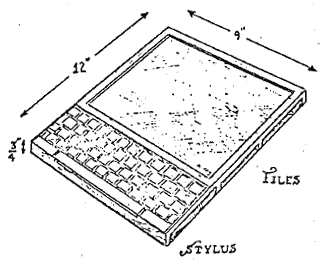
\includegraphics[width=10cm]{slike/dyna_skica.png}
\end{center}
\caption{Ilustracija modela Dynabook, 1972~\cite{kay}.}
\label{pic1}
\end{figure}


\section{Kaj ni mobilno učenje?}
\label{2.1}
Zaradi razširjenosti prenosnih in tabličnih računalnikov v  zadnjih letih, se je dojemanje pojma "mobilne tehnologije" nekako zameglilo. Čeprav se e-učenje pogosto uporablja kot sinonim za mobilno učenje, se med seboj razlikujeta v več pogledih. Mobilno učenje je izkušnja in priložnost, ki jo omogoča razvoj tehnologij na področju učenja. Pristop k učenju se je spremenil v takojšen dostop do vsebin na zahtevo uporabnika. Kar naredi mobilno učenje drugačno od ostalih načinov izobraževanja je to, da se lahko dogaja kadarkoli, kjerkoli in na načine, ki so drugačni kot pri e-učenju, kjer oseba sedi in komunicira z učiteljem ali računalnikom.\\ Glavne razlike med mobilnim učenjem in e-učenjem so:
\begin{itemize}
\item čas dogajanja,
\item dostop do informacij,
\item kontekst,
\item ocenjevanje,
\item podpora zmogljivosti,
\item uporabniško ustvarjena vsebina in
\item načrtovanje v skladu z zmogljivostjo mobilnih tehnologij.
\end{itemize}
Prva večja razlika med mobilnim ter e-učenjem je čas dogajanja. Večina e-učnih vsebin je narejena tako, da učenec sedi za računalnikom in napreduje skozi snov v nekem časovnem okvirju. Mobilno učenje po naravi ni omejeno s časom izvajanja, ali krajem kjer se učenje izvaja, ampak se uporablja po potrebi in razpoložljivosti uporabnika. Ker so zasloni ponavadi manjši, so zato tudi učne vsebine časovno krajše, saj uporabniki nočejo strmeti ure in ure v telefon, da bi zaključili začrtane cilje. \\ Mobilno učenje je zato primerno za posredovanje manjših kosov informacij oziroma vsebin, ki jih lahko uporabimo medtem ko čakamo prijatelja, stojimo v vrsti v trgovini ali pa na delovnem mestu. \\Naslednja razlika je dostop do informacij. Kadar opravljamo tečaj, ki je zasnovan kot e-učenje, je cilj, da je vsebina razumljiva in da si jo zapomnimo, dokler je ne bomo potrebovali. Pri mobilnem učenju je večkrat cilj, da dostopamo do informacij v trenutku, ko jih rabimo in ni toliko pomebno, da nam ostanejo v spominu. Kot primer lahko vzamemo hiter vodič po konfiguracijskih ukazih omrežnih naprav. Naloga inženirja je implementacija zaščite oddaljenega dostopa do usmerjevalnika pri stranki. Ker je bil tečaj na katerem je vadil konfiguriranje naprav obsežen, si ni zapomnil vseh ukazov, zato uporabi telefon na katerem ima naložena navodila z ukazi, s katerimi si lahko hitro pomaga in reši problem.\\Kontekst je eden ključnih področij, kjer se mobilno učenje in e-učenje razlikujeta. Pri e-učenju je potrebno vsebino postaviti v kontekst, da učenec razume pomembnost predmeta učenja. Pri mobilnem učenju je ponavadi kontekst že vzpostavljen. Na vodenem tečaju naprimer, je kontekst učenja vzpostavljen preko zgodbe, ki opisuje namen pridobljenega znanja. Pri mobilnem učenju, kjer ponavadi dostopamo do vsebine, ko jo potrebujemo, je uporabnik večinoma že postavljen v določen kontekst in je namen učenja očiten. Eden od intuitivnih načinov opredelitve konteksta je, da uporabniku prikažemo vsebino, ki je relevantna glede na lokacijo na kateri se nahaja. Kontekst lahko opredelimo tudi s časom dostopa do informacij, kjer naprimer določimo vsebino glede na dostop med jutranjim časom, delovnikom ali večernim časom.\\Za ocenjevanje lahko pri obeh načinih učenja uporabimo Kirkpatrickov model ocenjevanja usposabljanj in izobraževalnih programov~\cite{Kirkpatrick}. Ocenjevanje temelji na štirih stopnjah. To so odziv na usposabljanje, pridobljeno znanje, vedenje pri uporabi znanja in rezultat usposabljanja. Stopnje lahko v grobem razdelimo na dva dela. Prvi dve stopnji odgovorita na vprašanje "ali je bilo usposabljanje dobro", drugi dve stopnji pa odgovorita na vprašanje "ali so se učenci kaj naučili". Na prvo vprašanje je lažje odgovoriti pri e-učenju s pomočjo vprašalnikov. Težje je pri e-učenju preveriti drugo vprašanje, torej vedenjske spremembe učencev oziroma kako bodo znanje uporabili pri delu. Pri mobilnem učenju je praktično uporabo znanja lažje ugotoviti, saj ga, za razliko od e-učenja, ponavadi uporabljamo v trenutku, ko znanje potrebujemo pri delu.\\ Dostavljalec, ki ga zanimajo zadnji podatki o prometu na poti, ali pa zdravnik, ki želi ugotoviti informacije o kontraindikaciji zdravil, lahko s pomočjo mobilnih naprav enostavno dostopa do željenih podatkov. Zmožnost zajemanja ter deljenja informacij, ki ga mobilno učenje podpira, nam omogoča, da smo pri našem delu še bolj produktivni in zmogljivejši.
\\Tradicionalno je e-učenje enosmerno, torej učenci informacije prejemajo in jih ne delijo z ostalimi. Medtem, ko je vsebina e-učenja že nekako vnaprej določena in postavljena v učno okolje, je pri mobilnem učenju le ta bolj dinamična zaradi narave sodelovanja in socializiranja med uporabniki mobilnih naprav, zato je tudi več uporabniško ustvarjene vsebine.\\ Zadnja večja razlika med mobilnim in e-učenjem je zmogljivost naprav, ki omogočajo učenje. Prednosti, ki jih ima mobilno učenje pred ostalimi načini učenja, omogočajo tehnologije, ki niso na voljo v učilnicah in pri e-učenju. Funkcije kot so prikaz geografske lokacije naprave, kamera in senzorji gibanja, omogočajo veliko novih načinov učenja, kar za uporabnike naredi sistem bolj zanimiv, za razvijalce pa predstavlja nove izzive in možnosti izkoriščanja funkcij mobilnih naprav.

Mobilne naprave so prisotne povsod in postajajo vse bolj razširjene v vsakodnevnem življenju. Le malokrat se zgodi, da zapustimo dom brez, da bi s sabo vzeli telefon. Vse bolj odvisni postajamo od mobilnih naprav in velikokrat se ne zavedamo koliko jih uporabljamo za učenje.\\
Mobilno učenje je posledica rasti prodaje pametnih telefonov in tablic. V veliko držav si nekateri ljudje ne morejo privoščiti prenosnega računalnika, lahko pa si privoščijo pametni telefon. Še en vzrok za vse večjo uporabo mobilnega učenja je ta, da smo ljudje vedno v pogonu in zato iščemo načine, kako se učiti brez, da bi bili vezani na čas ali učilnico. Čas, ko smo na poti in smo nedejavni je lahko z uporabo mobilnega učenja tudi produktiven.

\section{Mobilne učne vsebine}
Učna vsebina, ki jo lahko uporabniki označijo kot mobilno, je lahko skoraj karkoli, do česar lahko dostopamo preko mobilnih naprav za potrebe formalnega ali neformalnega učenja. To so lahko naprimer tudi spletne strani, ki niso izključno namenjene izobraževanju.

Verjetno najenostavnejši način za pridobivanje takšnih informacij so tekstovna sporočila~\cite{MLcat}. Tekstovna ali SMS sporočila se lahko uporabijo za pošiljanje kratkih informacij na uporabnikovo zahtevo, tehnologija se je nekoč izkazala za dobro predvsem pri učenju jezikov~\cite{ItSMS}. Poleg enosmernih tekstovnih sporočil se za izmenjavo učnih vsebin uporablja tudi dvosmerna komunikacija, kjer uporabnik lahko pošlje povratno informacijo v bazo podatkov, kar se lahko uporabi pri vprašalnikih ali anketah. Mobilno učenje je lahko predstavljeno tudi v obliki zvočnih zapisov, predstavitvenih vsebin kot so diapozitivi, animacije, informacije, iz različnih podatkovnih baz, ki jih uporabnik zahteva v danem trenutku, video vsebine, ki so lahko prenesene na napravo ali pa predvajane preko interneta. \\Najlažje pa si mobilno učenje predstavljamo kot interaktiven medij za namensko učenje v obliki aplikacij, ki jih lahko naložimo na telefon ali dostopamo do njih preko spleta.

\section{Dostop do mobilnih vsebin}
Mobilne vsebine lahko uporabniku predstavimo na več načinov. S stališča dostopa do vsebine je ta lahko dostopna preko aplikacij, ki jih namestimo na mobilne naprave in so razvite za operacijske sisteme, ki tečejo na napravah, ponavadi za Android in IOS. Drugi način je dostop preko spletnih aplikacij za katere potrebujemo samo internetni brskalnik in po potrebi še vtičnike. 

Oba načina imata svoje prednosti in slabosti. Prednost spletnih aplikacij je v neodvisnosti od platforme, kar omogoča uporabnikom dostop ne glede na OS, ki je nameščen na mobilni napravi. S tem je vsebina na voljo širši publiki kot pri aplikacijah, ki potrebujejo namestitev. 
Obstajajo tudi hibridne aplikacije, ki tečejo na spletu in na mobilnih napravah obenem. Do aplikacije za učenje jezikov Duolingo lahko dostopamo preko namenske aplikacije ali pa spletne aplikacije, kot prikazuje slika~\ref{web_native}.
\begin{figure}[H]
\centering
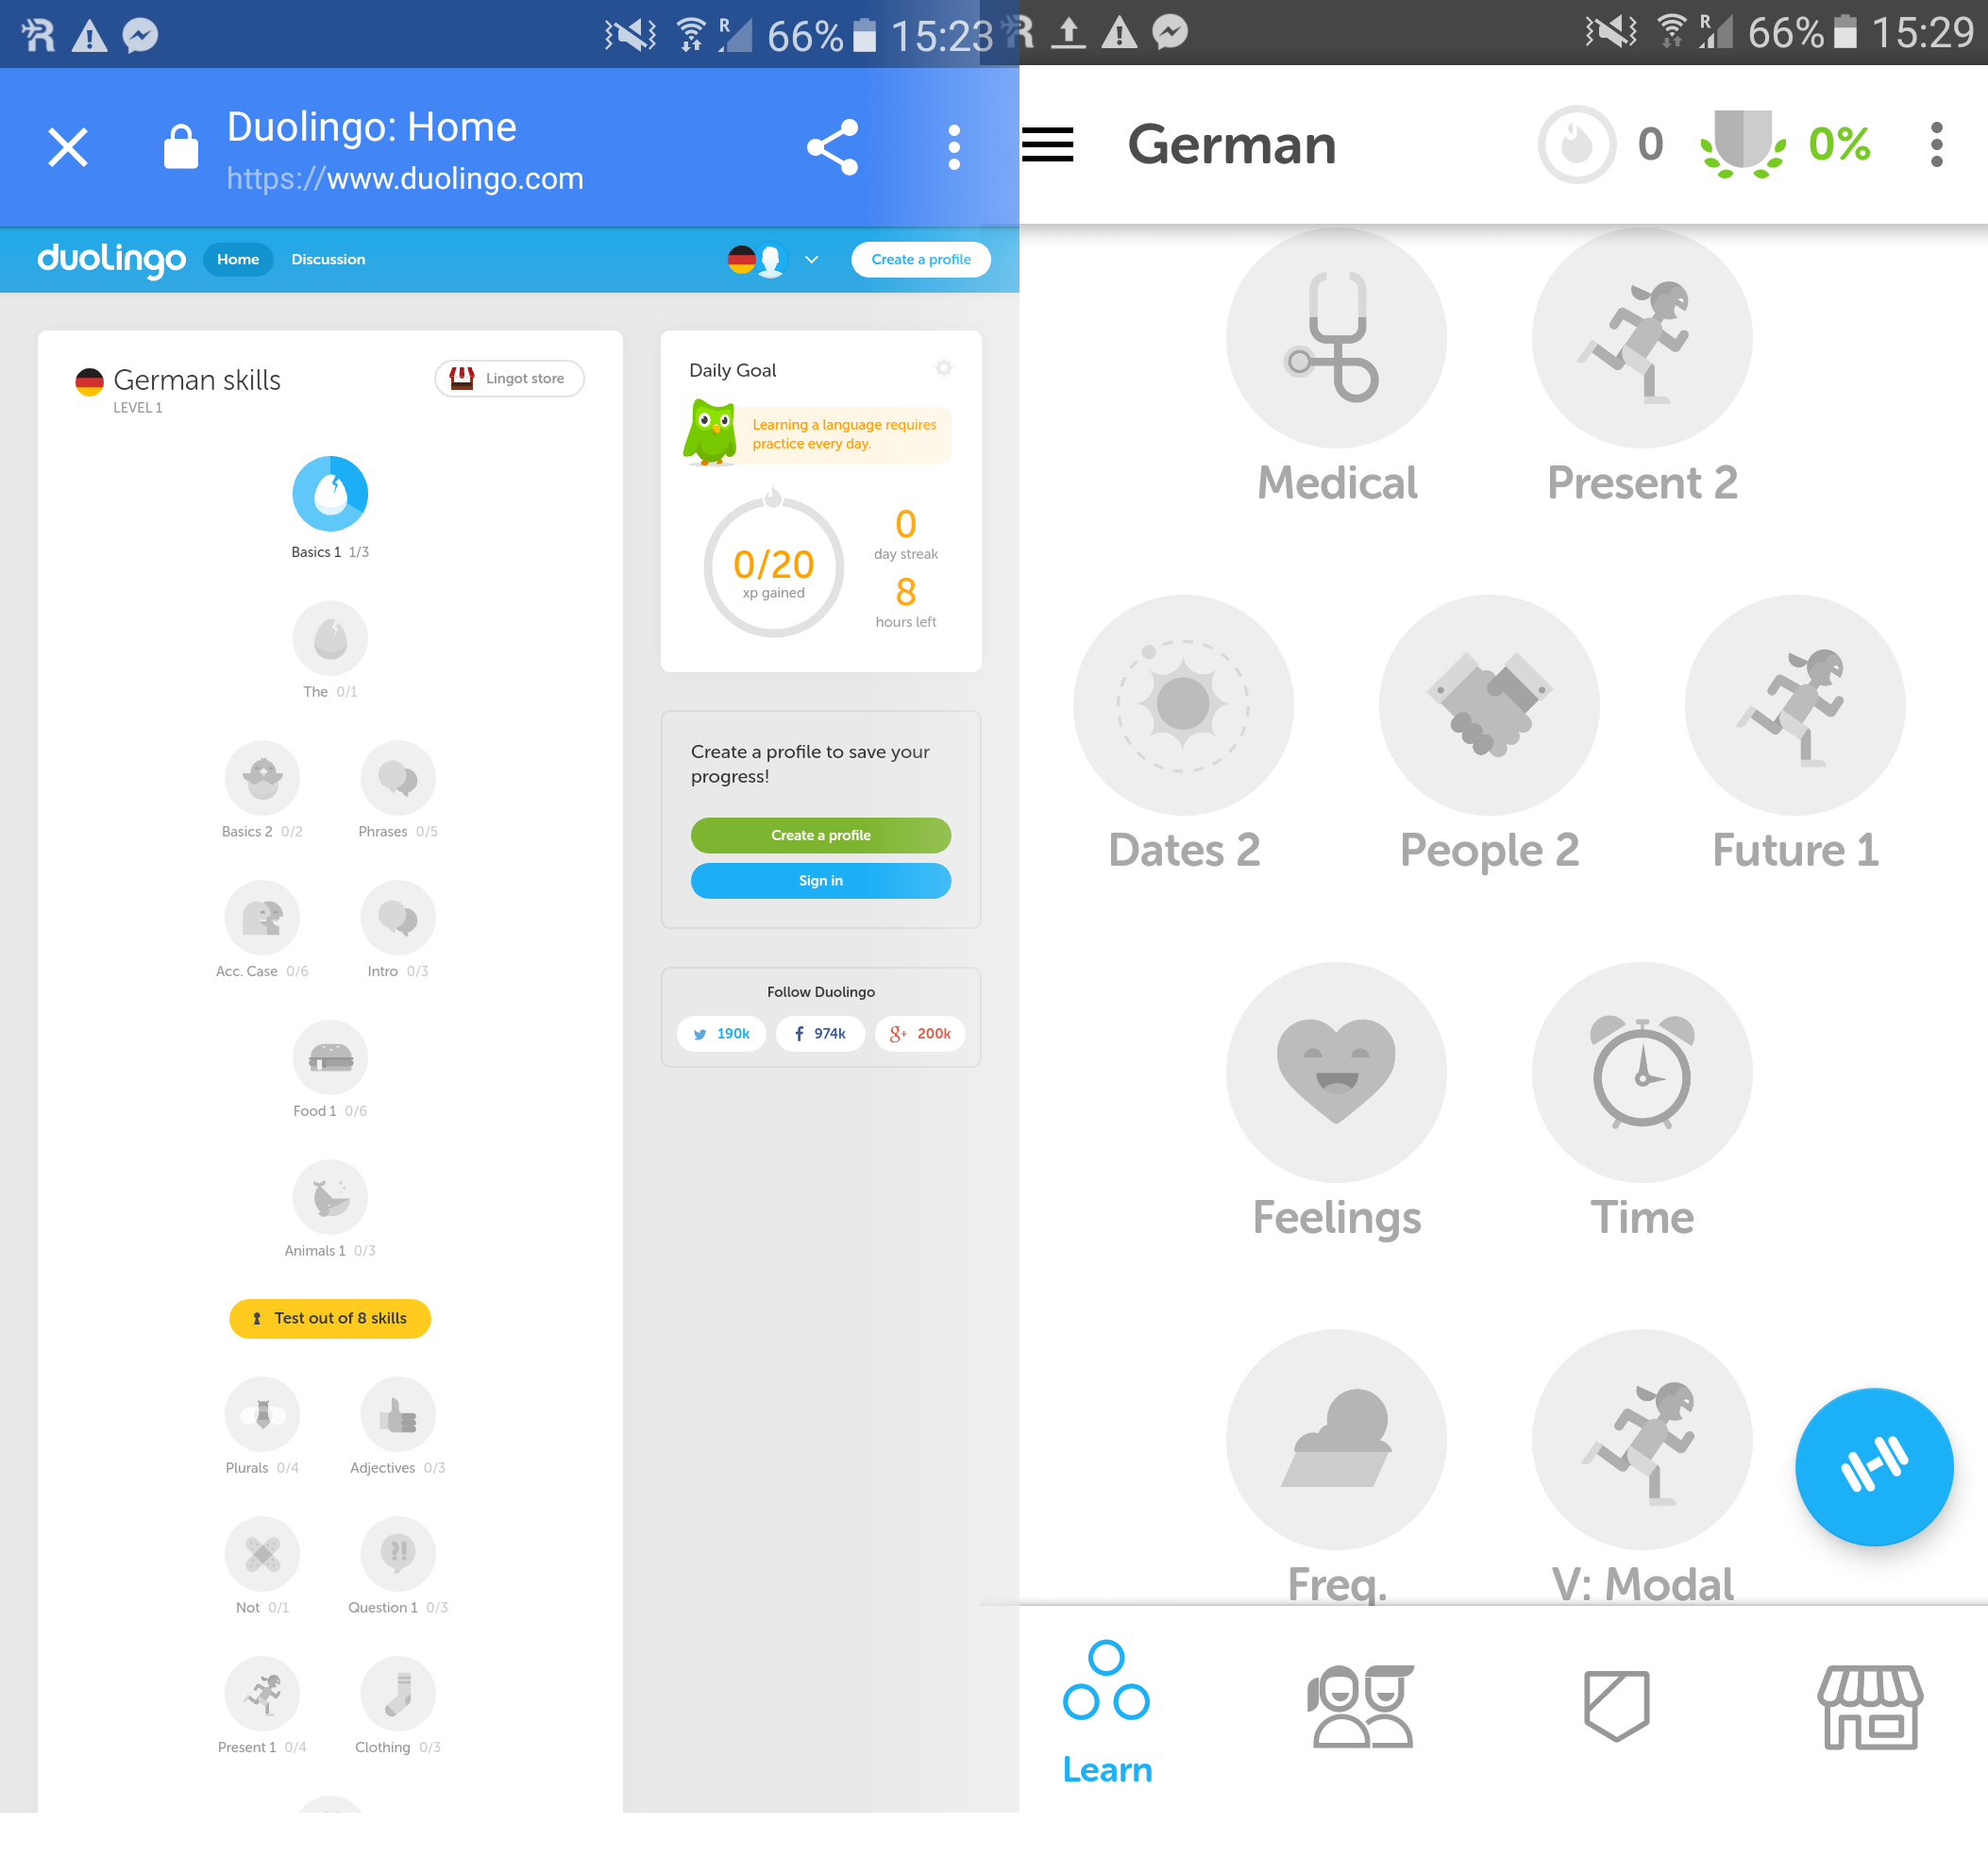
\includegraphics[height=0.7\textwidth]{slike/duoduo}
\caption{Primerjava spletne in nameščene aplikacije Duolingo}\label{web_native}
\end{figure}
Prednosti aplikacij, ki jih namestimo, so v dostopu do funkcij telefona in večinoma boljši uporabniški izkušnji. Čeprav lahko tudi pri razvoju spletnih aplikacij vključimo veliko funkcij naprav kot so kamera, GPS, mikrofon in ostale~\cite{cando}, so še vedno bolj podprte in lažje obvladljive pri razvoju aplikacij za točno določeno platformo. Pri obeh potrebujemo dostop do interneta, bodisi zaradi vsebine, bodisi zaradi podatkovne baze kamor se shranjujejo ali iz koder se pridobivajo uporabniške akcije.
\chapter{Gamifikacija in mehanika iger}
\label{ch3}
Izraz gamifikacija je postajal popularen iskalni niz v drugi polovici leta 2010~\cite{trend}, vendar njegovi začetki segajo v leto 2002, ko je svetovalec Nick Pelling z njim opisal uporabniški vmesnik za hitrejše in bolj prijetne elektronske transakcije na bankomatih, prodajnih avtomatih in mobilnih telefonih~\cite{conundra}. Izraz je od takrat ostal vendar se je njegov pomen spremenil.

Različne skupine ljudi si lahko gamifikacijo predstavljajo na različne načine. Prisotna je pri reklamiranju produktov ali storitev, tako kot je to Nike naredil z aplikacijo Nike+ Run, kjer lahko uporabniki spremljajo svoj napredek ter se primerjajo in tekmujejo z ljudmi po svetu, lahko je uporabljena pri ustvarjanju virtualnih svetov, ki motivirajo spremembo vedenja, pri učenju kompleksnih sistemov, ali pa kot metoda za vzpodbujanje učenja v formalnem ali neformalnem izobraževanju.\\
Gamifikacijo lahko za naše potrebe definiramo kot \textit{uporabo mehanike iger in načrtovanja digitalne izkušnje za motivacijo ljudi pri doseganju ciljev}~\cite{gargame1}.\\Mehanika iger predstavlja osnovni gradnik gamificiranega sistema. Orodja, ki so del mehanike iger, kot so točke, lestvice in stopnje lahko na različne načine vključimo v sistem, da ustvarimo uporabniško izkušnjo kot jo poznamo v igrah.\\
Danes so igre, gamifikacije in simulacije že skorajda povsod. Od iger, ki jih igramo preko spleta, da si prislužimo promocijske majice, pa vse do resnih vojaških iger za urjenje. Tudi na delovnih mestih in v izobraževalnih ustanovah je uporaba gamifikacije že sprejemljiva praksa.\\Razlogov zakaj postaja gamifikacija bolj pogosta je več. Izdelava iger je veliko lažja kot nekoč, obstajajo programi, ki olajšajo izdelavo enostavnih iger. Generacije, ki so odraščale z igrami so danes del podjetij in ustanov, zato tudi upada stigma do vpeljevanja takšnih pristopov učenja. Igre so na voljo na mobilnih telefonih, to omogoča, da uporabniki do njih dostopajo kjerkoli, kar spodbuja zanimanje za igre. Z vključevanjem iger v vsakdanje življenje se tako neposredno širi tudi uporaba gamifikacije. 

Mehanika gamificiranega sistema je sestavljena iz več orodij, ki ob pravilni uporabi predstavljajo prednost pred ne-gamificiranimi sistemi  in omogočajo boljšo uporabniško izkušnjo, ki uporabnika motivira, da doseže boljše rezultate. Predlagano je, da uporaba digitalnih iger, za namene izobraževanja, pozitivno vpliva na učne dosežke, razvoj kognitivnih sposobnosti, motivacijo in koncentracijo pri učenju~\cite{nint}.

\section{Točke}
Točke so lahko v gamificiranem sistemu uporabljene na različne načine. Z njimi nagradimo napredek in pravilne odgovore, uporabljene so lahko za odklepanje vsebin in kot valuta za kupovanje virtualnih dobrin.
Ko pomislimo na točkovni sistem nam največkrat pade na misel točkovanje v športu, računalniških igrah ali pa točke dodeljene uporabnikom za uspešno opravljene naloge znotraj igre.
Gamificiran sistem brez točkovanja praktično ne more obstajati.


Točkovanje v računalniških igrah poznamo vsi. Prisotno je v skoraj vsaki igri in indicira položaj igralca oziroma koliko je oddaljen od naslednje stopnje, v kakšnem položaju so soigralci ali koliko mu manjka, da igro zaključi.\\
Tudi številke na socialnih omrežjih predstavljajo neke vrste točkovanje. Uradne strani glasbenikov, športnikov ali pa posameznikov, z vsebino zanimivo za uporabnike na Facebooku, Youtube-u in podobnih socialnih omrežjih, vodijo evidenco koliko ljudi se zanima za njihovo stran, ali pa koliko všečkov je prejela objava in tudi to je neke vrste točkovni sistem.
Pri načrtovanju točkovnih sistemov bomo v diplomskem delu obravnavali 4 tipe točk za različne primere uporabe. Poglejmo si jih v nadaljevanju:
\begin{itemize}
\item \textbf{Izkušenjske točke}\\
Vse kar uporabnik naredi znotraj sistema, se prišteva k izkušnjam in načeloma se te točke nikoli ne odštevajo in se ne morejo vnovčiti. V nekaterih sistemih se lahko ponastavijo po nekem časovnem intervalu, če so cilji sistema tako zastavljeni, nimajo pa definirane maksimalne vrednosti.

\item \textbf{Spretnostne točke}\\
Spretnostne točke so bonus točke, ki jih uporabnik zasluži z sodelovanjem v dodatnih aktivnostih. Z njimi usmerjamo igralca k reševanju nalog, ki so navezane na glavno aktivnost, vendar niso obvezne za napredovanje. Z njimi lahko popestrimo proces mobilnega učenja. 

\item \textbf{Karma točke}\\
Te točke se ponavadi ne pojavljajo v klasičnih igrah. Uporabnik nima koristi, če jih obdrži, zato jih včasih podari ostalim tekmovalcem.  Njihov namen je lahko nagrajevanje za dobro opravljeno delo, ne da bi spremenili položaj igralca v igri. Prav tako se na ta način poveča pozitivna interakcija med uporabniki gamificiranega sistema. Pri mobilnem učenju so takšne točke lahko dodeljene, če je naprimer uporabnik določeno število zaporednih dni uporabljal aplikacijo.

\item \textbf{Vnovčljive točke}\\
Ta vrsta točk je namenjena za zamenjavo z nečim koristnim znotraj danega sistema, zato njihova vrednost niha. Uporabnik takšne točke zasluži in jih porabi. Služijo kot nekakšna virtualna valuta in imajo velikokrat temu primerna imena kot so virtualen denar, kovanci in podobno, lahko pa je ime tudi izmišljeno in se navezuje na tematiko sistema. Vnovčljive točke prinašajo tudi veliko vprašanj z legalnih in regulativnih stališč, vendar jih v diplomskem delu ne bomo obravnavali. Slika~\ref{duolingo2} prikazuje kako v aplikaciji Duolingo nakupujemo dobrine z virtualno valuto Lingo.
\end{itemize}
\begin{figure}[H]
\centering
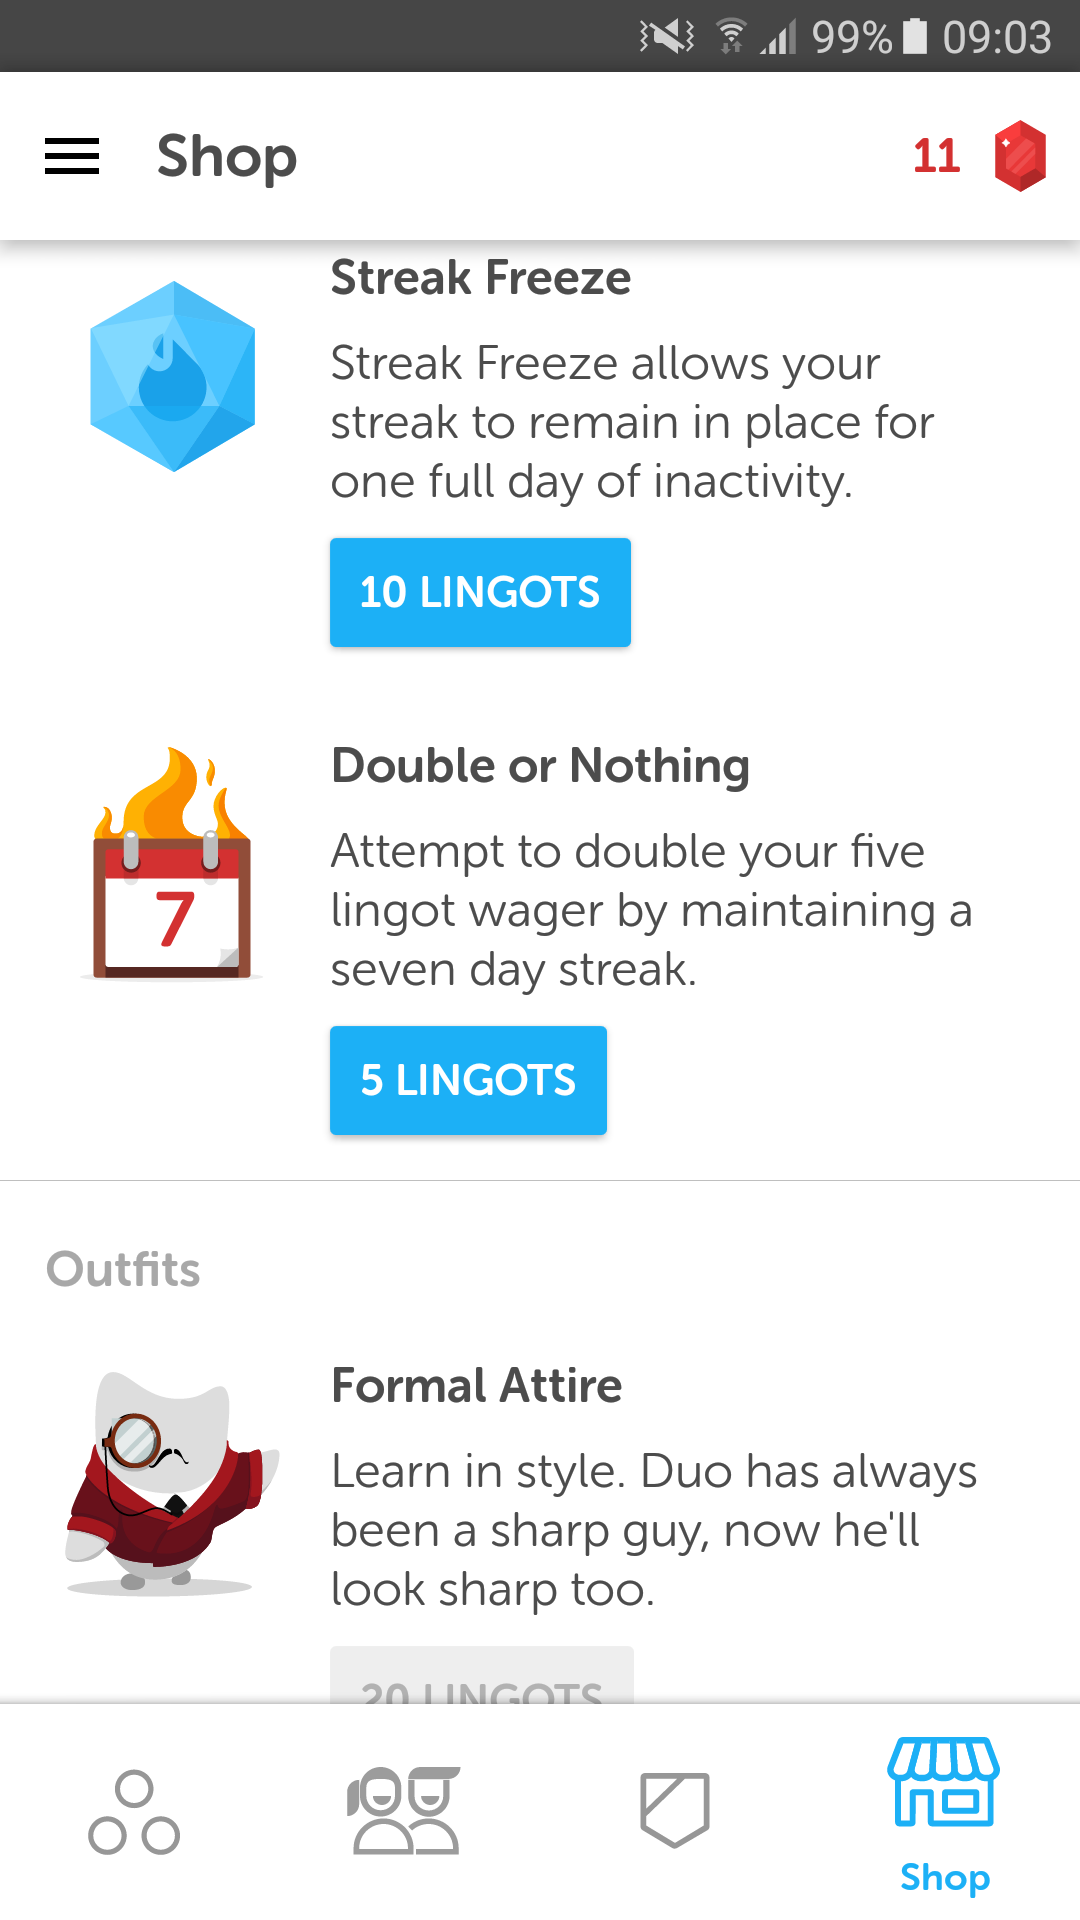
\includegraphics[height=0.8\textwidth]{slike/lingo}
\caption{Duolingo trgovina}\label{duolingo2}
\end{figure}

\section{Stopnje}
V večini iger stopnje nakazujejo napredek in čeprav ne moremo prenesti logiko stopenj iz računalniških iger neposredno v gamificirano učenje, je prav, da razumemo kako delujejo, saj so tudi pomeben del gamifikacije.\\Pri razvoju iger upoštevamo, da težavnost ne narašča linearno. Pri prehajanju v višje stopnje poskušamo nekatere naloge narediti lažje, torej težavnost narašča v obliki nekakšne krivulje. Lahko tudi naredimo nekatere stopnje bistveno težje, kot so to naredili razvijalci pri igri Angry birds, kjer je stopnjo 21 možno zaključiti samo na en način. Veliko igralcev je obupalo, zato je bil izziv zanimivejši in za tiste, ki jim je uspelo, občutek, da so dosegli nekaj posebnega, še toliko večji.

Tako kot je občutek napredka pomemben pri igrah, je tudi pri učenju. Če oseba ne dobi občutka, da je učenje produktivno, hitro izgubi interes. Učenci in študenti dobijo med izobraževanjem, z opravljanjem domačih nalog in ocenjevanjem, vpogled kako so napredovali pri določeni temi, nimajo pa poti napredka skozi celoten proces dela. Pri mobilnem učenju je ta proces lažje spremljati, saj so ponavadi stopnje točno definirane in vsebujejo večje število nalog, ki so krajše in za katere ob reševanju dobimo takojšnjo povratno informacijo o uspešnosti, za kar je potrebno pri formalnem izobraževanju ponavadi čakati dlje časa. Čeprav poznamo več vrst točkovanj, vseeno poskusimo ustvariti enostaven sistem točkovanja, ki uporabnika ne bo zmedel.

\section{Lestvice}
Namen lestvic je, da prikažejo primerjave med igralci po točkah doseženih v igri. Biti morajo dovolj preproste, da ne potrebujejo posebne razlage in, da igralcu predstavijo podatke tako, da ga spodbujajo k nadaljnjemu igranju. Če je pričakovano število igralcev veliko, je dobro, da je lestvica prilagojena in ne prikazuje samo seznama vseh urejenih od najboljšega do najslabšega, saj to z strani uporabnika aplikacije mogoče ni najbolj spodbudno. Če se uporabnik primerja s svojimi prijatelji oziroma z manjšo skupino ljudi ima lahko več zagona, da nadaljuje saj prikažemo relativen položaj uporabnika, kar pomeni, da je na lestvici recimo 5 boljših in 5 slabših posameznikov, katerih dosežki so lažje dosegljivi.\\ Če gre za večje število uporabnikov je mogoče smotrno, da rezultate razdelimo po več lestvicah, in sicer lokalno, po socialnih omrežjih in globalno. Lokalna lestvica prikaže uporabniku primerjave z ljudmi iz njegove okolice, socialna prikaže primerjave z rezultati uporabnikovih prijateljev na socialnih omrežjih ali pa znotraj aplikacije, globalna pa je lestvica, ki vsebuje vse uporabnike.

\section{Značke}
Značke so v vsakdanjem življenju prisotne že veliko časa. Najdemo jih na različnih mestih, saj z njimi označujemo avtomobile, vojska nagrajuje vojake z medaljami in čini, uporabniki mobilnih aplikacij pa zbirajo značke različnih restavracij in lokalov, ki so jih obiskali.\\
Zbiranje značk je dober način motiviranja ljudi. Dobro oblikovana značka je lahko zanimiva že samo zaradi dizajna. Odvisno od sistema, jih lahko uporabimo za spremljanje napredka namesto stopenj.\\
Na sliki~\ref{duolingo} vidimo kako aplikacija Duolingo uporablja značke, ki nakazujejo katera področja je uporabnik že osvojil oziroma katerih še ni.
\begin{figure}[H]
\centering
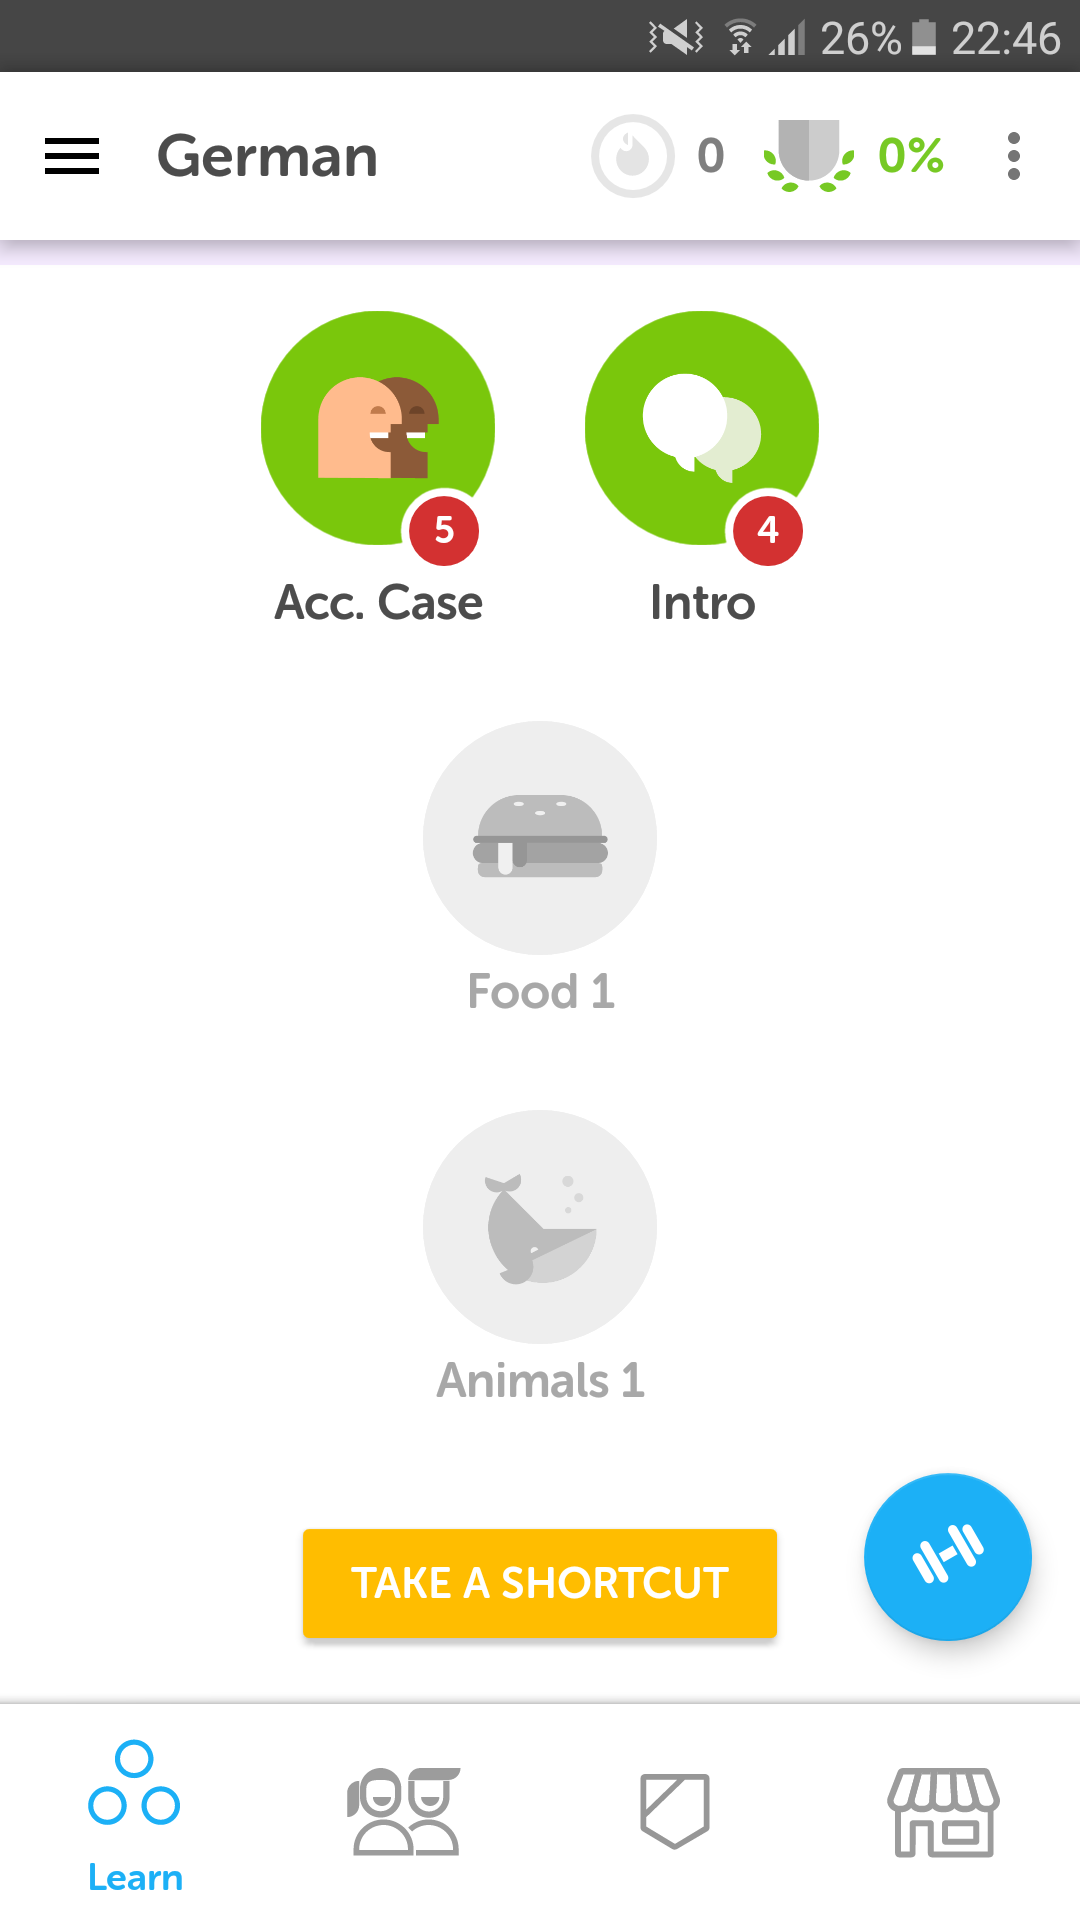
\includegraphics[height=0.7\textwidth]{slike/duolingo}
\caption{Duolingo značke za napredek}\label{duolingo}
\end{figure}

\noindent Poleg spremljanja napredka se značke dodeljuje tudi za dosežke, ki s samo vsebino niso neposredno povezani. Naprimer, če je uporabnik rešil zaporedno 5 kvizov brez napake, ali pa, če je vsak dan skozi mesec uporabljal aplikacijo.

Načinov kako pri mobilnemu učenju vključiti značke je več, vendar je smiselnost odvisna od samega sistema mobilnega učenja in njegove vsebine. Če ne uporabljamo učenja po korakih oziroma področjih, kot je to primer pri učenju jezikov v Duolingu, je uporaba značk za prikaz napredka vprašljiva, zato raje uporabimo pasico napredka in stopnje.

\chapter{Funkcije mobilnih naprav kot orodja za gamifikacijo mobilnega učenja}
\label{ch4}

Mobilne naprave so že dosegle zmogljivosti osebnih računalnikov in poleg zmogljivosti ponujajo funkcije in lastnosti, ki pripomorejo k boljši uporabniški izkušnji pri mobilnem učenju. Te naprave uporabljajo mehanizme za interakcijo kot so zasloni na dotik in različni senzorji, kot je naprimer senzor pospeška. Ti omogočajo bolj naravno komunikacijo kot je bilo prej mogoče na osebnih računalnikih. Večja izbira funkcij pomeni več možnosti za razvijalce pri načrtovanju gamificiranih mobilnih sistemov.

Razumeti moramo, da senzorji in ostale funkcije ne pogojujejo gamifikacije na mobilnih napravah. Ta lahko obstaja tudi brez uporabe le teh. Pripomorejo pa k boljši izvedbi funkcionalnosti, ki nastopajo v gamificiranem sistemu in omogočajo uporabo metod kot so lokacijsko določena vsebina in razpoznavanje zajete slike, kjer so senzorji uporabljeni za določanje konteksta učenja oziroma so podatki iz senzorjev predmet učenja.

 
\section{Kamera}
Ljudje radi ustvarjamo video vsebine in objavljamo slike na popularnih socialnih omrežjih in platformah kot so Instagram, Facebook in Youtube. Koliko vsebin je namenjenih učenju je težko ugotoviti, saj omenjene strani niso namenjene izključno izobraževanju, vseeno pa lahko na njih najdemo veliko poučnih vsebin.

Posnetke in slike, ki jih s kamero zajamemo, lahko uporabimo na različne načine. Poleg objavljanja na socialnih medijih so lahko uporabljeni za prikaz obogatene resničnosti - tehnologija, ki doda tekst ali virtualne objekte sliki, na katero je kamera fokusirana. Pri mobilnem učenju je lahko uporabljena za prikaz dodatnih informacij v realnem času na zajeti sliki ali pa za prevajanje besedila v trenutku, s snemanjem objektov, kot to omogoča Google Prevajalnik~\cite{translate}.\\Slika~\ref{Gtranslate} prikazuje prevod besedila z uporabo obogatene resničnosti v aplikaciji Google Prevajalnik.
\begin{figure}[H]
\centering
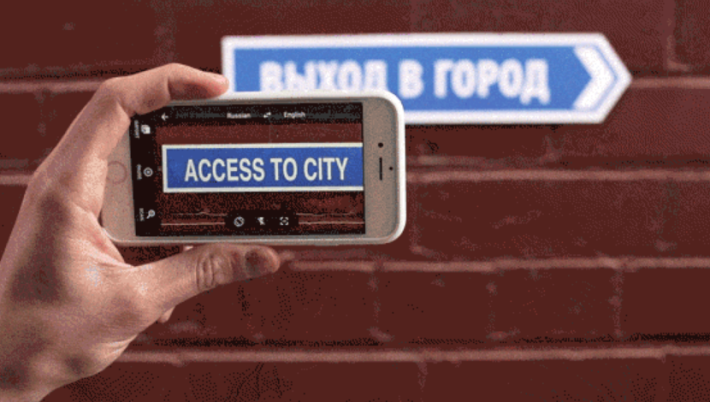
\includegraphics[height=0.5\textwidth]{slike/translate}
\caption{Google Prevajalnik slik~\cite{GpictureTr}}\label{Gtranslate}
\end{figure}

\noindent Kamera na mobilnih napravah je uporabna tudi za skeniranje QR kod, ki prikažejo dodatne informacije o objektu, naprimer navodila za uporabo orodja, ali pa za razpoznavo objektov na sliki, kot naprimer počne aplikacija Leafsnap, ki omogoča učenje listov dreves na podlagi zajetih slik.\\Vsekakor je kamera uporabno orodje mobilnih naprav, ki je primerna za uporabo v mobilnem učenju, saj lahko olajša delo in poskrbi za dinamično interakcijo med aplikacijo in uporabnikom.
\section{GPS}
Globalni sistem pozicioniranja se uporablja za lokacijske storitve, kar omogoča natančno določanje lege objektov na zemlji. GPS je bil ena prvih funkcij na telefonih, ki se je medtem izboljšala in se uporablja na mobilnih napravah na različne načine. Najbolj značilna je uporaba pri aplikacijah za navigacijo, za prikaz uporabnikove lokacije in določanje smeri do želenega cilja.

GPS je v aplikacijah omogočil uporabo funkcionalnosti kot so omogočanje uporabnikom, da se prijavijo (check-in) na lokacijah in to delijo s prijatelji, najdejo ocene restavracij v bližini in dodajanje geo-oznak pri objavi slik na socialnih omrežjih. Lokacijo lahko uporabimo tudi pri mobilnem učenju na več načinov. Če zbiramo podatke na način, da jih uporabniki vnašajo v aplikacijo in nas pri tem zanima izvor podatkov, lahko uporabimo lokacijo naprave, da spremljamo s kje so bili podatki posredovani. Firefly Counter~\cite{firefly} je takšen primer aplikacije, kjer uporabniki po vsej državi spremljajo populacijo kresnic in posredujejo podatke preko mobilne aplikacije. Raziskovalci na podlagi podatkov in izvora le teh, ugotavljajo vzroke za rast ali padec populacije.

Uporaba geo-oznak je metoda, ki jo lahko uporabimo za označevanje uporabniško generirane vsebine. S tem naredimo povezavo med vsebino in lokacijo na katero se ta vsebina nanaša. Tako so naprimer na univerzi DePaul v ZDA študentje s pomočjo aplikacije Evernote, ki omogoča avtomatsko dodajanje geo-oznak k zapiskom, naredili voden ogled zgodovinsko pomembnega pokopališča~\cite{evernote}. GPS lahko uporabimo tudi za t.i. geofencing~\cite{geofence}, pri čemer aplikacija zazna, ko naprava vstopi v določeno, prednastavljeno območje na zemljevidu, pri čemer se sproži implementirana akcija. S tem lahko uporabniku prikažemo informacije o kraju v katerega je prišel, ali o objektih v bližini katerih se je uporabnik pojavil. Če želimo lestvice pri gamificiranem mobilnem učenju prikazati glede na okolico uporabnika, si tudi pomagamo z lokacijskimi storitvami.
 
Učenje pri katerem se zavedamo konteksta okolice in kjer ta postane del učne vsebine, lahko motivira učence, da raziskujejo in znanje uporabijo v resničnih situacijah. V preteklosti je bilo takšno učenje povezano z učenjem izven učilnice, obiskovanjem muzejev in parkov, z razvojem mobilnih tehnologij pa se je takšna oblika učenja preselila tudi na mobilne naprave. Z lokacijskimi storitvami lahko zagotovimo, da prikažemo primerne podatke glede na trenutno lokacijo uporabnika, kar pride prav v veliko primerih pri mobilnem učenju in gamifikaciji.
\section{Glasovna kontrola}
Eden prvih senzorjev na mobilnih napravah je bil mikrofon, ki služi za glasovno komunikacijo v mobilnih telefonih. Danes mikrofon najdemo tudi na ostalih mobilnih napravah kot so tablice in pametne ure, kjer se lahko na različne načine uporablja za upravljanje vsebin na napravah.\\Glasovna kontrola je lahko zelo uporabna pri mobilnem učenju in se jo da kreativno uporabiti, če želimo gamificirati proces učenja. Inteligentni osebni asistent Google Now in aplikacijski programski vmesnik Voice Actions na Android napravah omogočata kontrolo mobilne naprave z glasom. Glasovno kontrolo na Android napravi aktiviramo z zlogom "OK Google", nakar naprava čaka na nadaljnje ukaze. S pretvorbo govora v tekst (STT) in teksta v govor (TTS) lahko upravljamo z navigacijo, pošiljamo tekstovna sporočila, predvajamo glasbo, nastavimo alarm, preverimo vremensko napoved in še veliko več~\cite{now}. Na voljo je več aplikacijskih programskih vmesnikov kot so Google Directions, Google Places, Google Calendar ipd., ki nam vse to omogočajo.\\\ Uporaba glasovne kontrole je vsekakor primerna tudi za invalide, ki mobilne naprave ne morejo uporabljati s klasičnimi metodami. Temu primerne so lahko tudi aplikacije za mobilno učenje.

\section{Senzorji gibanja}
Vključitev senzorjev gibanja v aplikacije za mobilno učenje omogoči uporabnikom bolj raznoliko uporabo naprav in več interaktivnosti ter občutka sodelovanja v aktivnosti z gibanjem telesa.

Žiroskop in senzor pospeška v mobilnih napravah omogočata unikatno funkcinalnost pri igrah in simulacijah. Uporabniki lahko z žiroskopom merijo nagibe, obračanja in zavoje, kar lahko uporabimo kot 3-dimenzionalen kontroler s katerim upravljamo aplikacijo. Senzor pospeška meri spremembo hitrosti, v mobilnih napravah se meritve izvajajo na treh oseh, kar omogoča, da naprava zazna smer premikanja podobno kot pri žiroskopu.\\Aplikacija StarWalk~\cite{starwalk} uporablja senzorje gibanja s katerimi lahko uporabnik premika pogled na virtualno nebo z obračanjem mobilne naprave. 
Skupaj z magnetnim senzorjem, ki omogoča delovanje kompasa in lokacijskimi storitvami, prikaže uporabniku zvezdno nebo iz uporabnikove perspektive. Z uporabo obogatene resničnosti se lahko učimo imena in pozicije zvezd, ter planete na nebu, prav tako pa se prikazujejo orisi ozvezdij.
Z žiroskopom in senzorjem pospeška lahko razvijemo zanimivo uporabniško izkušnjo pri mobilnem učenju, vendar včasih je z nagibanjem in obračanjem naprave težje upravljati aplikacijo, zato je potrebno poznati končne uporabnike in razmisliti o smiselnosti uporabe senzorjev gibanja, preden jih implementiramo.\\Slika~\ref{starwalkpic} prikazuje primer uporabe aplikacije StarWalk za učenje nebesnih teles.
\begin{figure}[H]
\centering
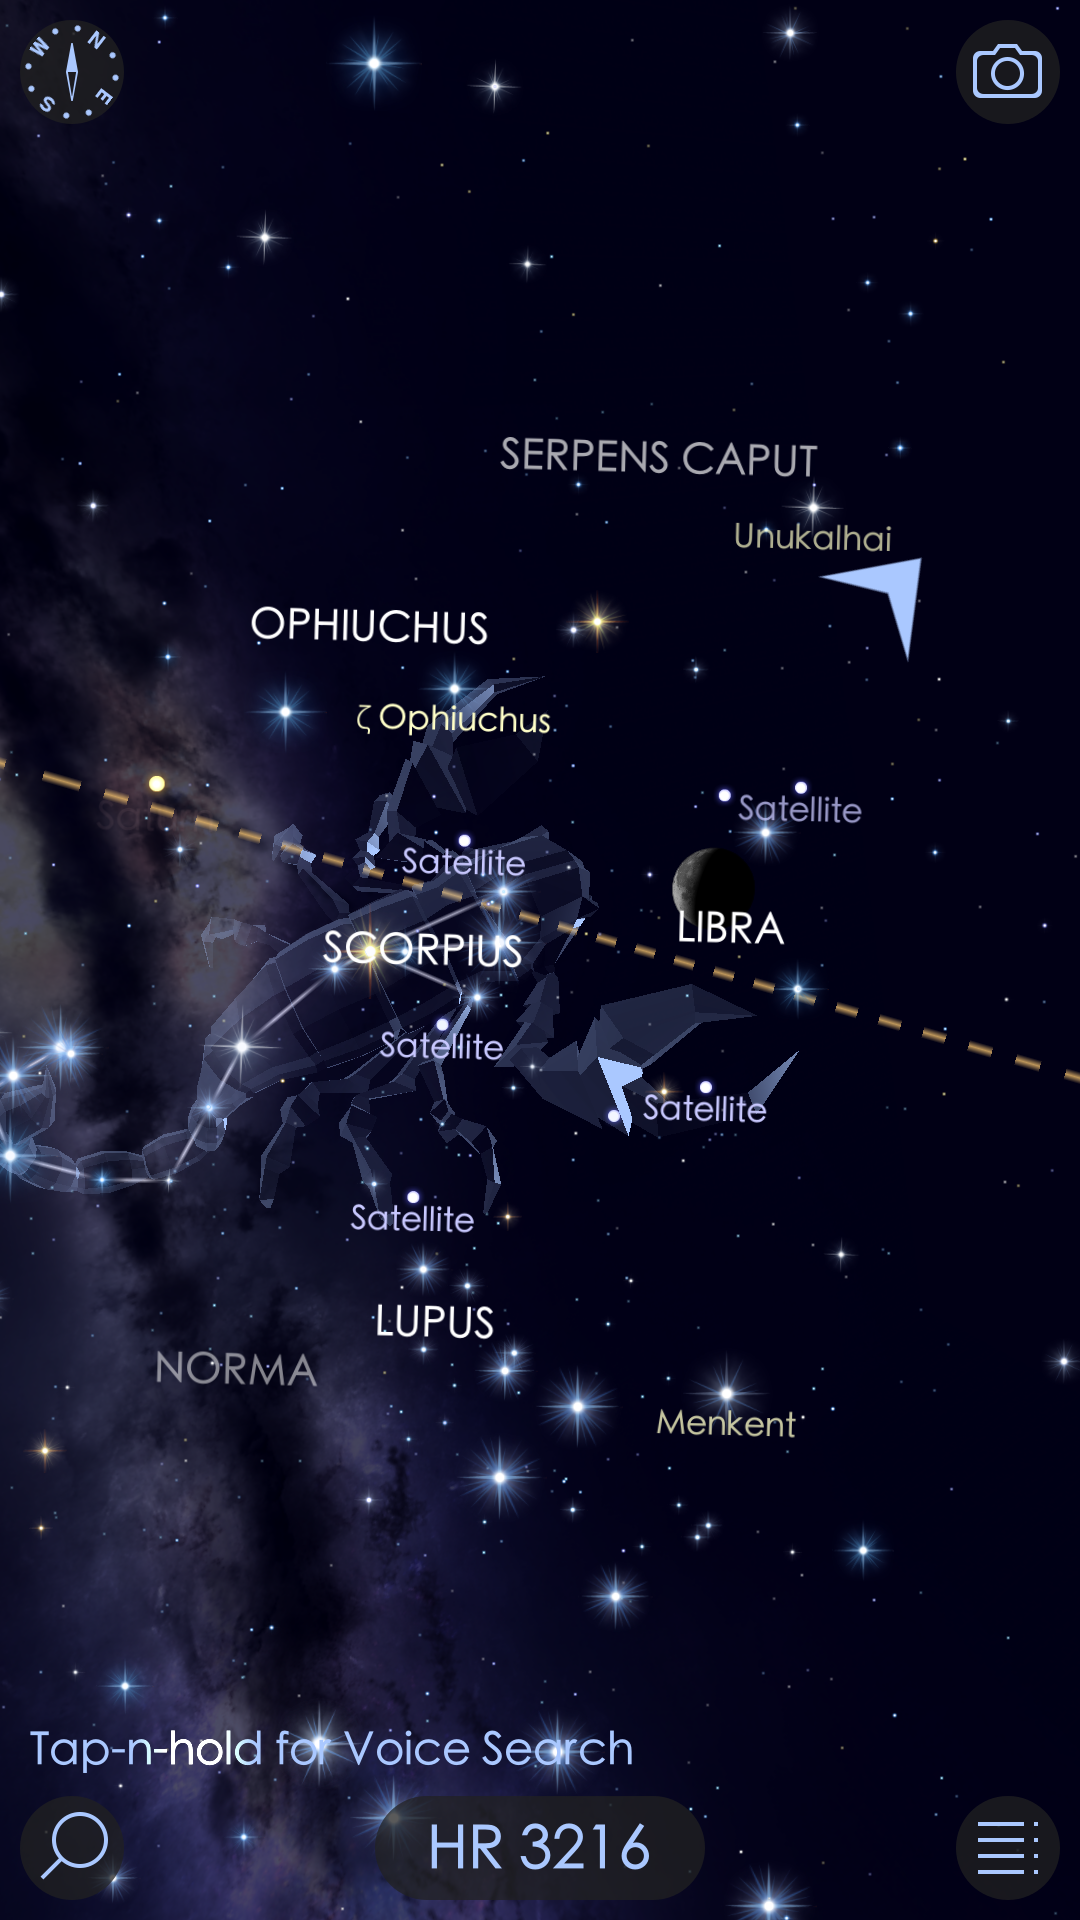
\includegraphics[height=0.8\textwidth]{slike/starwalk}
\caption{Aplikacija StarWalk 2}\label{starwalkpic}
\end{figure}
 
\section{iBeacon}
IBeacon je standard, ki ga je razvilo podjetje Apple. Napravam, ki podpirajo protokol za brezžično komunikacijo bluetooth omogoča, da prejemajo ali oddajajo informacije preko radio signala BLE~\cite{BLE}. Oddajniki signala nenehno oddajajo signal, ki vsebuje njhovo natančno lokacijo in identifikator. Prejemniki signala lahko na podlagi teh informacij ugotovijo, kje v prostoru se nahajajo. V aplikaciji na tak način prikažemo bistvene podatke o uporabnikovi okolici. Takšna vrsta prepoznavanja območja je podobna kot pri GPS-u, a se razlikuje po vrsti tehnologije in namenu, saj so iBeaconi bolj primerni za manjša območja, naprimer prikazu popustov, ko nakupovalec hodi med nakupovalnimi policami.\\
V izobraževalne namene so iBeacon oddajniki lahko nameščeni v galerijah in muzejih pri razstavnih eksponatih, da opozorijo aplikacijo, da prikaže uporabnikom ustrezne informacije, kot so video, slike in avdio vodiči. Takšna vrsta informacij lahko izboljša splošno izkušnjo in uporabnika vodi do  relevantnih podatkov. Na takšen način iBeacon standard izkorišča gamificirana aplikacija za učenje, slovenskih razvijalcev, Nexto~\cite{nexto}.

\chapter{Razvoj aplikacije}
\label{ch5}
Razvili smo sistem za mobilno učenje z uporabo gamifikacije. Sistem sestavljata dve uporabniški aplikaciji, mobilna in spletna. Namen uporabe obeh ni enak, vendar se med seboj dopolnjujeta. Želeli smo omogočiti dodajanje vsebine, do katere bodo dostopali uporabniki mobilne aplikacije, zato smo razvili spletni portal. Nanj se lahko prijavimo in ustvarjamo nove izzive in naloge za uporabnike, ter jih tudi urejamo.\\Podatke, ki so ustvarjeni na portalu, smo naredili dostopne preko aplikacijskega vmesnika, kamor mobilna aplikacija pošilja zahteve za dostop do vsebine. Odgovor aplikacijskega vmesnika na zahtevo, ki je v obliki json, na mobilni aplikaciji oblikujemo in prikažemo na uporabniškem vmesniku.\\V nadaljevanju bomo opisali uporabljene tehnologije, probleme s katerimi smo se srečali in kako smo jih rešili.
\section{Tehnologije in orodja}
Za izdelavo diplomskega dela smo uporabili tehnologije, ki so bile izbrane glede na zahteve projekta. Ker smo naredili spletno in mobilno aplikacijo, je bilo potrebno izbrati programske jezike, ter orodja, ki so nam olajšala delo na projektu. Izbrali smo jih na podlagi prejšnjih izkušenj in poznavanja posameznih tehnologij in orodij.
\subsection{HTML}
HTML oziroma Hyper Text Markup Language, je označevalni jezik za katerega razvoj skrbi mednarodni inštitut W3C~\cite{w3c}. Narejen je za izdelavo spletnih strani in je osnoven gradnik le teh. Opisuje in definira vsebino spletnih strani, za kar uporablja različne značke, ki določajo format v katerem se bo besedilo prikazalo. Med takšne značke sodijo \textless head\textgreater, \textless title\textgreater, \textless body\textgreater, \textless article\textgreater, \textless div\textgreater, ter številne druge. Trenutna najnovejša različica je HTML 5.1~\cite{html}.
\subsection{PHP}
PHP je programski jezik, ki je lahko uporaben za različne namene, posebej pa je primeren za razvoj spletnih aplikacij. Uporabimo ga lahko skupaj s HTML označevalnim jezikom, za razvoj dinamičnih spletnih strani. PHP izvorna koda je izvršena na strežniku, rezultat pa je pretvorjen v HTML, ki je nato posredovan odjemalcu.\\V našem primeru smo ga skupaj s HTML jezikom uporabili pri pisanju uporabniškega portala, saj smo potrebovali dinamično spletno aplikacijo, kjer lahko generiramo novo vsebino na zahtevo. Vnose uporabnika v spletno aplikacijo lahko obdelamo s PHP programskim jezikom, jih shranimo v podatkovno bazo in nato prikažemo rezultat uporabniku.\\Za razvoj smo uporabili PHP ogrodje Laravel, opisano v poglavju~\ref{laravelsubs}, ki je zgrajeno na podlagi PHP jezika in vsebuje pomožne elemente, ki olajšajo delo pri pisanju kode. Najnovejša različica PHP programskega jezika je 7.1.

\subsection{CSS}
CSS ali v prevodu kaskadne stilske podloge, je jezik za pisanje slogovnih predlog. Z njim lahko oblikujemo predstavitev dokumenta oziroma spletne strani, napisane v HTML jeziku. Določimo lahko barve, velikost, poravnave in postavitve elementov na spletnih straneh~\cite{css}.\\Oblikovanje spletnih strani je v sodobnih časih pomemben vidik pri ustvarjanju dobre uporabniške izkušnje. Dobro oblikovana spletna aplikacija bo privabila več uporabnikov, ki bodo na njej preživeli več časa. Na voljo je veliko knjižnic z že prednastavljenimi oblikovnimi elementi, ki jih lahko vključimo v svojo izvorno kodo. Tudi za CSS skrbi inštitut W3C, trenutno najnovejša je 4. različica jezika.
\subsection{Javascript}
Sriptni jezik, ki nam omogoča, da spletne strani naredimo še bolj interaktivne in dinamične, se imenuje Javascript.\\Vključimo ga lahko v HTML spletno stran in ga uporabimo za nadgradnjo statične strani. Uporabljamo ga za animacijo elementov, preverjanje uporabniških vnosov in dinamično generiranje vsebine v aplikacijah. Z njim lahko ustvarimo tudi računalniško igro~\cite{JSgame}. Večina spletnih strani uporablja Javascript in vsi sodobni spletni brskalniki ga podpirajo. Pri razvoju odjemalskih aplikacij se uporablja standardizirana različica Javascripta, ki se imenuje ECMAScript~\cite{ES}, vendar pogovorno večina razvijalcev uporablja ime Javascript.
\subsection{Typescript}
Typescript je zastonjski odprtokodni programski jezik, ki ga je razvilo podjetje Microsoft. Je nadgradnja programskega jezika Javascript. Typescript je ob zagonu preveden v Javascript izvorno kodo kar pomeni, da je slednji podmnožica Typescripta, torej je izvorna koda, napisana v Javascript jeziku, veljavna Typescript koda.\\Omogoča definiranje razredov in vmesnikov, kot smo jih vajenih iz objektnih jezikov kot je C\#. Dodaja tudi možnost definicije tipov spremenljivk, velika prednost je tudi, da omogoča integriranim razvojnim okoljem lažje razpoznavanje napak in obveščanje o teh med pisanjem izvorne kode~\cite{typescript}.\\
V našem projektu smo ga uporabili pri razvoju mobilne aplikacije.

\subsection{Git}
Git je sistem za upravljanje z izvorno kodo, ki omogoča kontrolo nad različico in spremembami, narejenimi v izvorni kodi.\\Kadar na projektu sodeluje več razvijalcev, lahko z njim spremljamo napredek in delo posameznih razvijalcev. Ustvarimo lahko več t.i. vej, kjer lahko razvijalci pišejo svoje spremembe in popravke kode ne glede na ostale razvijalce, ter kasneje te veje združimo v glavno vejo, ki predstavlja izvorno kodo delujoče aplikacije. V večini časa je uporabljen za shrambo izvorne kode, tako se izognemo lokalno shranjenim različicam projektov in se lahko vrnemo na prejšnje različice kode, če je to potrebno.\\ Obstaja več spletnih aplikacij, kamor lahko prenesemo projekt s sistemom GIT, mi smo se odločil za Bitbucket, saj za razliko od bolj priljubljenega Github-a omogoča zastonjske privatne shrambe.

\subsection{REST}
Kako omogočiti aplikacijam dostop do podatkov, ki se nahajajo v podatkovnih bazah in strežnikih izven njihove domene? \\Arhitektura REST predstavlja način, kako vsak vir predstavimo kot spletno storitev z naslovom URL. REST določa uporabo protokola HTTP in njegovih standardnih metod:
\begin{itemize}
\item GET
\item PUT
\item POST
\item DELETE
\end{itemize}
Podobno kot delujejo spletni brskalniki, ki uporabljajo URL naslove za izvajanje zahtev na strežniku, tudi REST izkorišča HTML metode za pridobivanje podatkov iz strežnika. Tipičen primer uporabe REST storitev v spletnih aplikacijah je t.i. CRUD (Create, Update, Delete) oziroma ustvari, posodobi, izbriši, pri čemer mislimo na zapise v podatkovnih bazah.\\ Metodo GET uporabimo, kadar želimo pridobiti podatke od strežnika. Pri tej metodi moramo posredovati identifikator elementa, o katerem želimo prejeti informacije. Za pošiljanje podatkov na strežnik oziroma, kadar želimo shraniti podatke v podatkovno bazo, uporabimo POST metodo. Za posodabljanje obstoječih zapisov na strežniku, uporabimo metodo PUT, ki ji podobno kot pri GET metodi, posredujemo identifikator elementa. Za brisanje zapisa iz baze uporabljamo DELETE metodo.\\  V našem primeru smo REST arhitekturo uporabili za komunikacijo mobilne aplikacije s strežnikom, kjer so shranjeni podatki o izzivih in o samih uporabnikih. Za vsako zahtevo, ki potrebuje dostop do podatkov, ali pa želi podatke zapisati v bazo, obstaja URL naslov, ki poskrbi za komunikacijo s strežnikom. Implementirali smo avtentikacijo z žetoni, kar pomeni, da uporabniki ne morejo dostopati do podatkov, če niso avtenticirani v sistemu. 

\section{Knjižnice in ogrodja}
\subsection{Bootstrap}
Bootstrap je zastonjsko odprtokodno orodje za oblikovanje spletnih strani. Je orodje namenjeno izključno za oblikovanje prikaza sprednjih strani in ne omogoča uporabo v zalednih sistemih. Uporabljamo ga preko HTML predlog, ki so definirane v CSS oblikovni datoteki. Možna je tudi uporaba javascript razširitev, ki razvijalcu omogočajo ustvariti boljšo uporabniško izkušnjo.\\Z njim lahko naredimo prilagodljivo spletno stran, kar pomeni, da bo prilagojena velikosti zaslona na katerem aplikacijo pregledujemo. Ustvarili so ga razvijalci pri Twitterju, zato včasih zasledimo ime Twitter Bootstrap. Najprej je bil uporabljen kot interno ogrodje za socialno omrežje Twitter, nato so se odločili, da ga nadgradijo in dajo na voljo javnosti. Bootstrap predloge in komponente razume večina brskalnikov. Trenutno je na voljo 4. različica ogrodja.


\subsection{Laravel}
\label{laravelsubs}
Spletno aplikacijo, ki služi kot portal za dodajanje izzivov, smo napisali s pomočjo ogrodja Laravel.\\Laravel je zastonjsko odprtokodno spletno ogrodje, ki temelji na jeziku PHP in uporablja znani MVC arhitekturni vzorec za ločevanje pogleda in logike, ki teče v ozadju. Prednost njegove uporabe je prilagodljivost in dostopnost razširitev, ki omogočajo enostavno dodajanje funkcionalnosti. Avtentikacijo uporabnikov je tako mogoče dodati preko ukazne vrstice, podobno tudi razširitev za spletno plačevanje s karticami in še mnogo drugih funkcionalnosti~\cite{laravel}.\\Za delo z bazo uporablja Eloquent objektno-relacijsko preslikovanje. Eloquent je implementacija  aktivnega zapisa vzorca ali Active record pattern~\cite{activerecord}, kjer je tabela ali pogled predstavljen z objektom oziroma modelom, preko katerega dostopamo do podatkov ali pa jih v podatkovno bazo zapisujemo. Primer, kako Eloquent deluje, vidimo v spodnji kodi, kjer do vnosov v bazi dostopamo preko objekta uporabnika in njegovih atributov.
\begin{lstlisting}
public function takenChallenges($player)
{
    $player = Player::find($player);
    $takenChallenges = array();
    foreach ($player->challenges as $challenge) {
        $takenChallenges[] = $challenge->pivot->challenge_id;
    }  
    return response()->json(['data' => $takenChallenges], 200);
}
\end{lstlisting}
Laravel smo uporabili tako za aplikacijo za dodajanje vsebine, kot tudi za strežnik preko katerega z REST klici dostopamo do te vsebine.
\subsection{Ionic}
Ionic je odprtokodno ogrodje za razvoj mobilnih aplikacij z uporabo spletnih tehnologij HTML, CSS in Javascript. Čeprav v izvorni kodi uporabljamo programske jezike, ki so namenjeni izdelavi spletnih strani, lahko z vgrajenimi komponentami zgradimo aplikacijo, ki izgleda in deluje enako kot, če bi jo napisali naprimer v Javi s programskim paketom Android.

Ionic aplikacije so zgrajene s pomočjo Apache Cordova~\cite{cordova}. Cordova je ogrodje, ki spletno kodo pretvori v aplikacijo, ki preko aplikacijskega programskega vmesnika dostopa do vseh zmogljivosti naprave, kot so razni senzorji, podatki in podobno. Cordova aplikacije so implementirane s pomočjo WebView pogleda na Android platformi, ki je namenjen prikazovanju spletnih strani. Ionic aplikacija komunicira s pogledom WebView in Cordova vtičniki tako kot je prikazano na sliki~\ref{ionicArch}.
\begin{figure}[H]
\centering
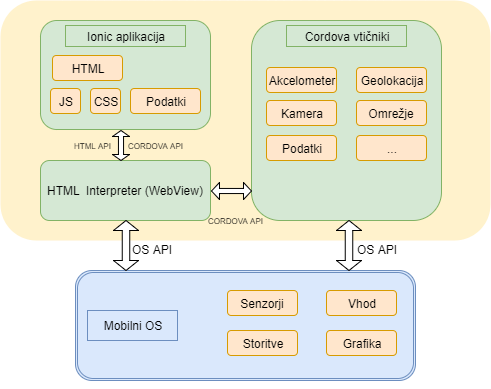
\includegraphics[height=0.7\textwidth]{slike/ionicArch}
\caption{Arhitektura Ionic aplikacije}\label{ionicArch}
\end{figure}

\noindent Aplikacije lahko razvijamo za mobilne operacijske sisteme iOS, Android, Blackberry in WP8. Izvorna koda Ionic aplikacij temelji na Angular platformi, njegovih razširitvah in stilskih CSS datotekah, namenjenim mobilnim napravam.

\section{Primeri aplikacij}
Razvijalci in pedagogi iščejo nove načine motiviranja ljudi pri učenju. Mobilne naprave, skupaj s poučnimi igrami, so lahko dober način motiviranja in povečanja aktivnosti učencev pri delu. V tem podpoglavju bomo predstavili nekaj dobrih primerov aplikacij, ki uporabljajo principe iger za učenje na mobilnih napravah. Z raziskovanjem obstoječih aplikacij na tem področju, smo pridobili ideje, ki so nam pomagale tudi pri razvoju našega sistema. 
\subsection{Duolingo}
Duolingo je platforma namenjena učenju jezikov~\cite{Duolingo}. Aplikacijo lahko uporabljamo preko spletnega brskalnika, ali pa jo namestimo na mobilno napravo. Uporabniki odgovarjajo na vprašanja v obliki kvizov, sestavljank besednih zlogov ter ustnih odgovorov, kjer aplikacija z razpoznavo govora preverja izgovarjavo besed. Sistem temelji na uporabi gamifikacije za motiviranje uporabnikov. Uporabniki z uspešnim reševanjem nalog prejemajo točke, ki se uporabijo za beleženje napredka pri posameznem jeziku oziroma področju. Za opravljanje nalog služimo tudi denar v obliki virtualne valute Lingo, ki ga lahko porabimo za kupovanje dodatnih nalog ali pa pomoči pri reševanju kvizov. Lestvice uporabniki ustvarjajo sami. Tako si jih lahko prilagodijo glede na skupino ljudi, ki se jezika uči skupaj. \\Za delo, ki ga uporabniki opravijo, prejemajo tudi različne značke. Slika~\ref{duo_znacke} prikazuje značko, ki je bila podeljena, ko smo uspešno rešili pet nalog brez napake.
\begin{figure}[H]
\centering
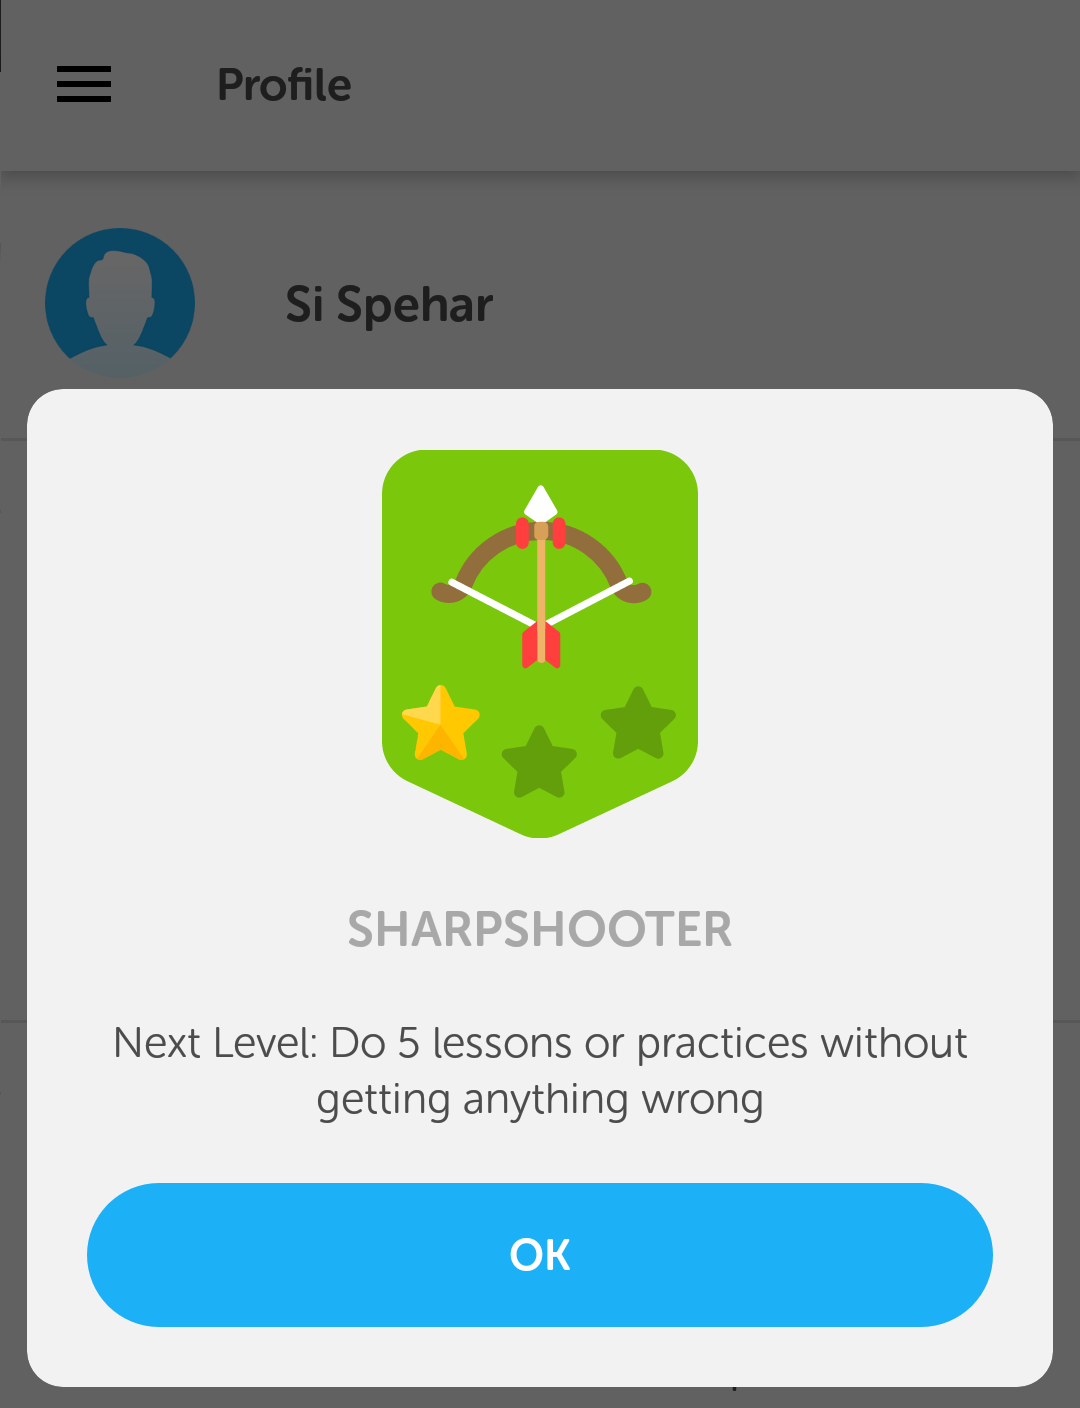
\includegraphics[height=0.7\textwidth]{slike/duo_znacka}
\caption{Primer značke v Duolingo aplikaciji}\label{duo_znacke}
\end{figure}
\noindent Leta 2017 je aplikacija imela okoli 200 milijonov uporabnikov, od tega jih je 25 milijonov mesečno aktivnih~\cite{Duolingo_stats}.

\subsection{Brainscape}
Brainscape je spletna in mobilna aplikacija, ki ponuja uporabnikom učenje različnih vsebin z uporabo tablic (flashcards)~\cite{Brainscape}. Uporabnik lahko v iskalniku najde temo, ki se jo želi naučiti, ali pa celo ustvari svojo preko spletnega portala. Po izbiri teme, se vrstijo vprašanja v obliki tablic. Na vprašanja uporabnik ne odgovarja z izbiro ali pa z vnosom pravilnega odgovora. Odgovor na vprašanje se v aplikaciji prikaže na zahtevo uporabnika, nato pa je njegova naloga, da na lestvici od 1 do 5 oceni, kako dobro ta odgovor pozna. 
Slika~\ref{brainscape} prikazuje primer, kjer je uporabniku prikazano vprašanje na katerega odgovori z izbiro stopnje, ki pove s kakšno gotovostjo bi uporabnik znal na vprašanje odgovoriti sam.
\begin{figure}[H]
\centering
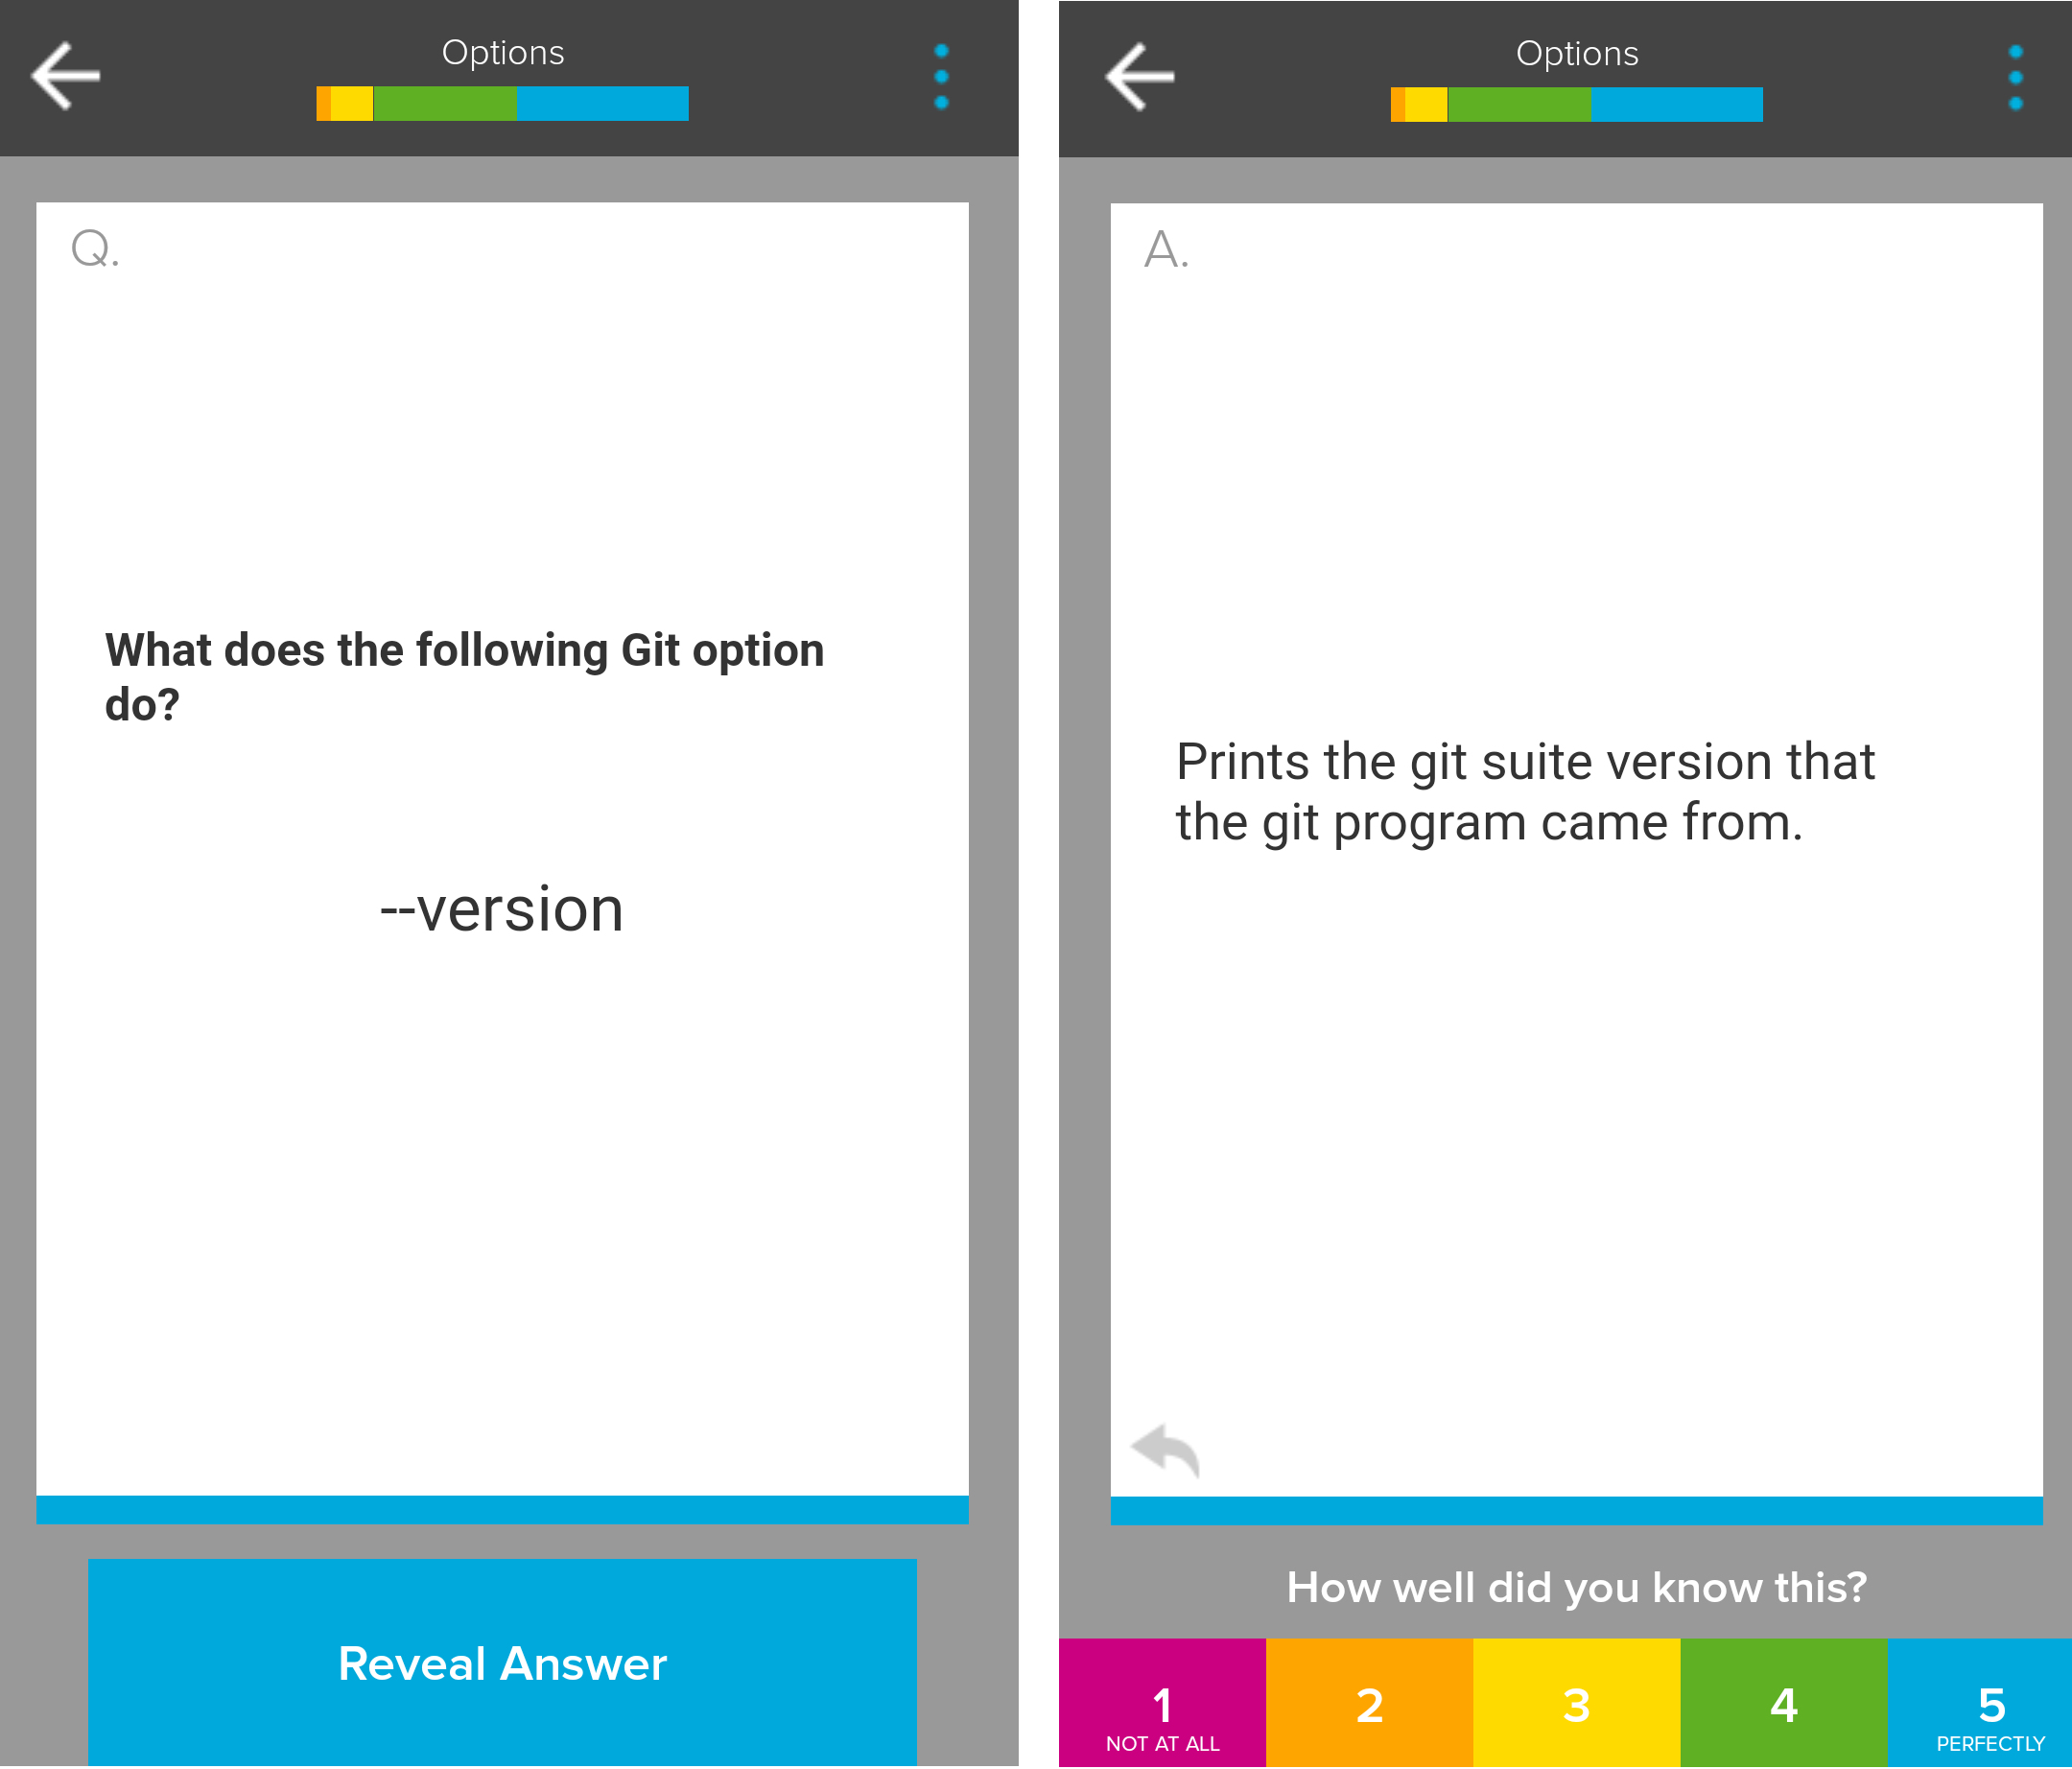
\includegraphics[height=0.7\textwidth]{slike/Brainscape}
\caption{Primer vprašanja in odgovora v Brainscape aplikaciji}\label{brainscape}
\end{figure}
\noindent Najbolj prepoznavna značilnost Brainscapa je algoritem ponavljanja, ki poskrbi, da se vprašanja, na katera uporabnik ne zna odgovoriti z veliko gotovostjo, večkrat ponovijo. Teme, oziroma vprašanja, ki jih uporabnik dobro pozna, se pojavljajo manj pogosto, tako se lahko uporabnik bolj osredotoči na vsebine, ki jih še ni osvojil. Algoritem ponavljanja na podlagi zaupanja, oziroma Confidence-Based Repetition, je podprt z raziskavo~\cite{cbr}, ki predlaga, da lahko na takšen način bolj izkoristimo čas učenja in hitreje pridobivamo znanje. V aplikaciji uporabniki z odgovarjanjem na vprašanja pridobivajo točke in tako spremljajo napredek pri posamezni temi. Vsaka izbrana tema ima tudi svojo lestvico, kjer se učenci lahko med seboj primerjajo.
\subsection{SoloLearn}
SoloLearn je brezplačna mobilna aplikacija za učenje programskih jezikov~\cite{Sololearn_app}. Uporabniki se lahko učijo programskih jezikov kot so Java, Python, C++, C\#, PHP, Javascript, kot tudi poizvedovalnega jezika SQL in označevalnega jezika HTML. Aplikacija ponuja tudi učne vsebine o podatkovnih strukturah, algoritmih in strojnem učenju. Poleg samostojnega učenja lahko uporabniki v vseh naštetih jezikih med seboj tekmujejo.\\Naloge posameznih jezikov so razdeljene na področja. Vsako področje vsebuje določeno število vprašanj, na katera lahko uporabniki odgovarjajo. Odgovori na vprašanja vsebujejo vnosna polja, kjer uporabniki dopolnejo manjkajočo kodo, ali pa so v obliki kviza, kjer uporabniki iz seznama izberejo pravilen odgovor. Slika~\ref{Python3} prikazuje pogled področij, ki se jih uporabniki lahko učijo v programskem jeziku Python.
\begin{figure}[H]
\centering
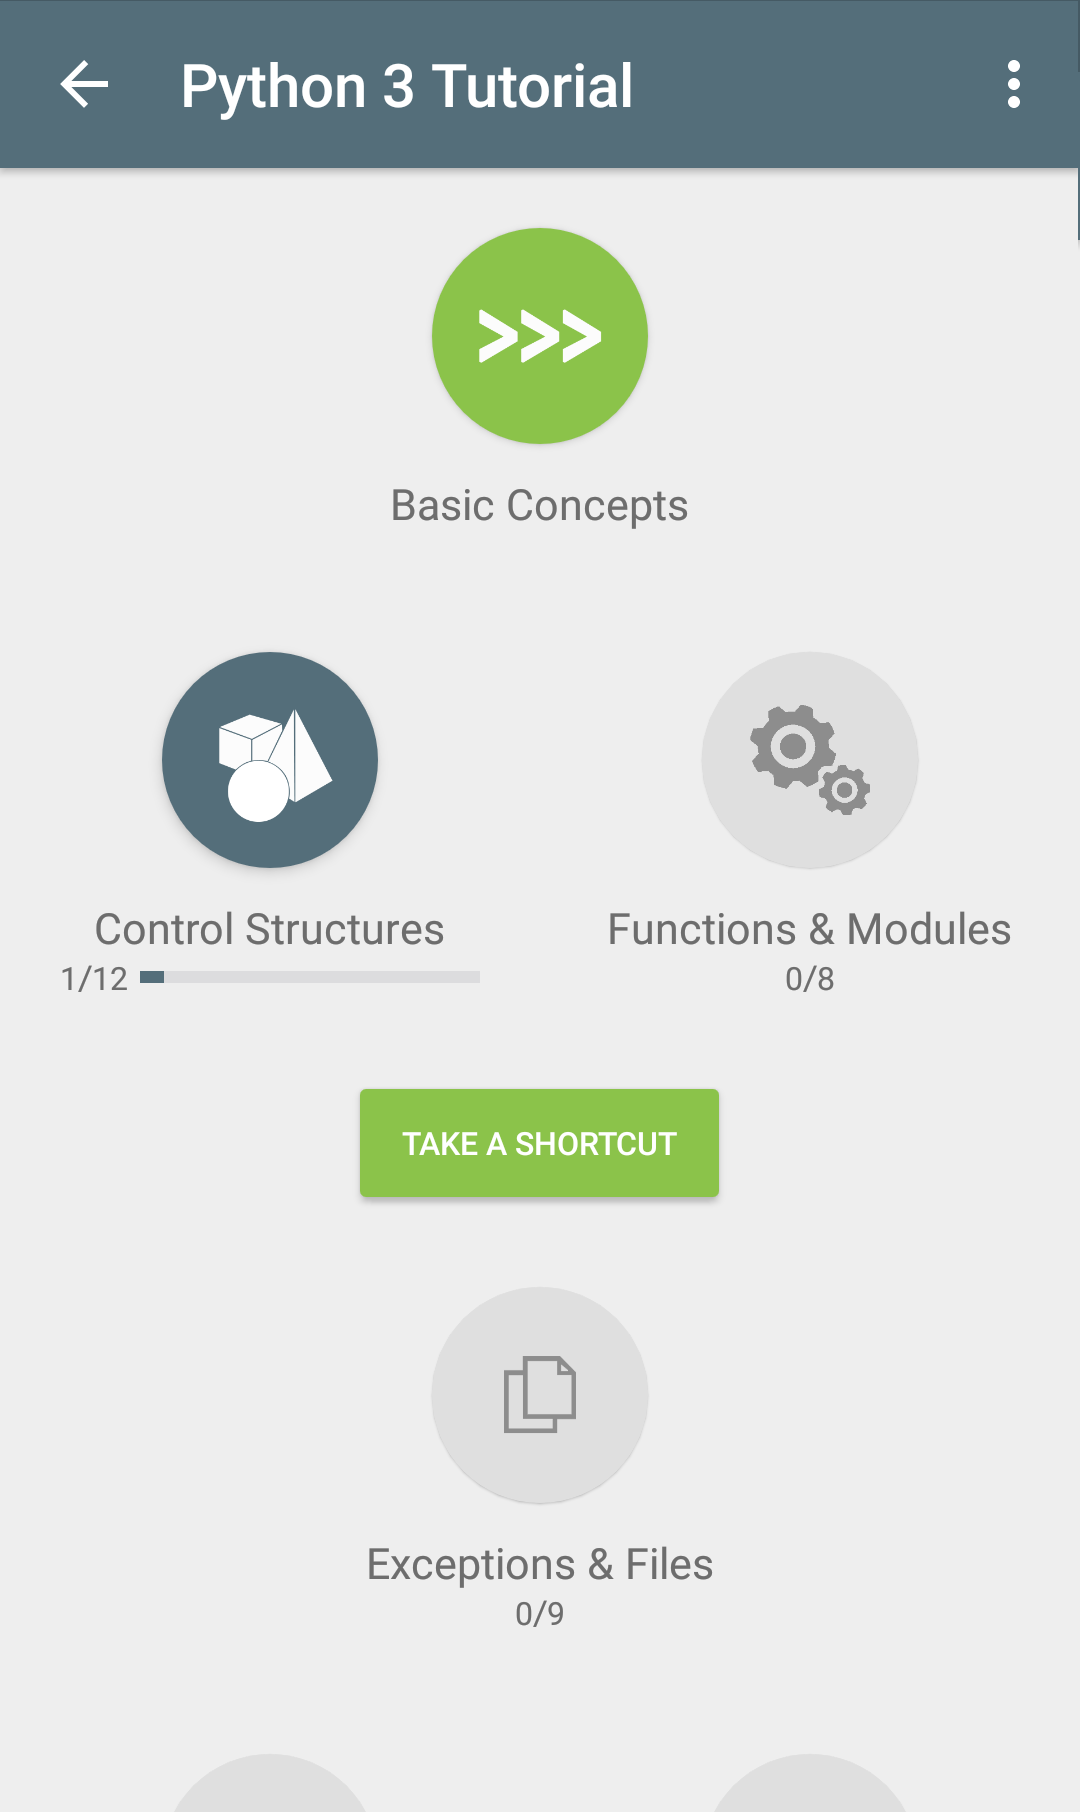
\includegraphics[height=0.7\textwidth]{slike/Python3}
\caption{Področja programskega jezika Python}\label{Python3}
\end{figure}
\noindent V aplikaciji lahko uporabniki med drugim objavljajo tudi svojo kodo, komentirajo kodo ostalih uporabnikov in sodelujejo v pogovoru z ostalimi uporabniki aplikacije.\\Na uporabnikovi osebni strani imamo pregled nad rešenimi nalogami, izzivi v katerih smo sodelovali, osvojenimi značkami in številom točk, ki jih potrebujemo za prehod v višjo stopnjo. Slika~\ref{sololearn} prikazuje uporabnikovo osebno stran z njegovimi aktivnostmi.

\begin{figure}[H]
\centering
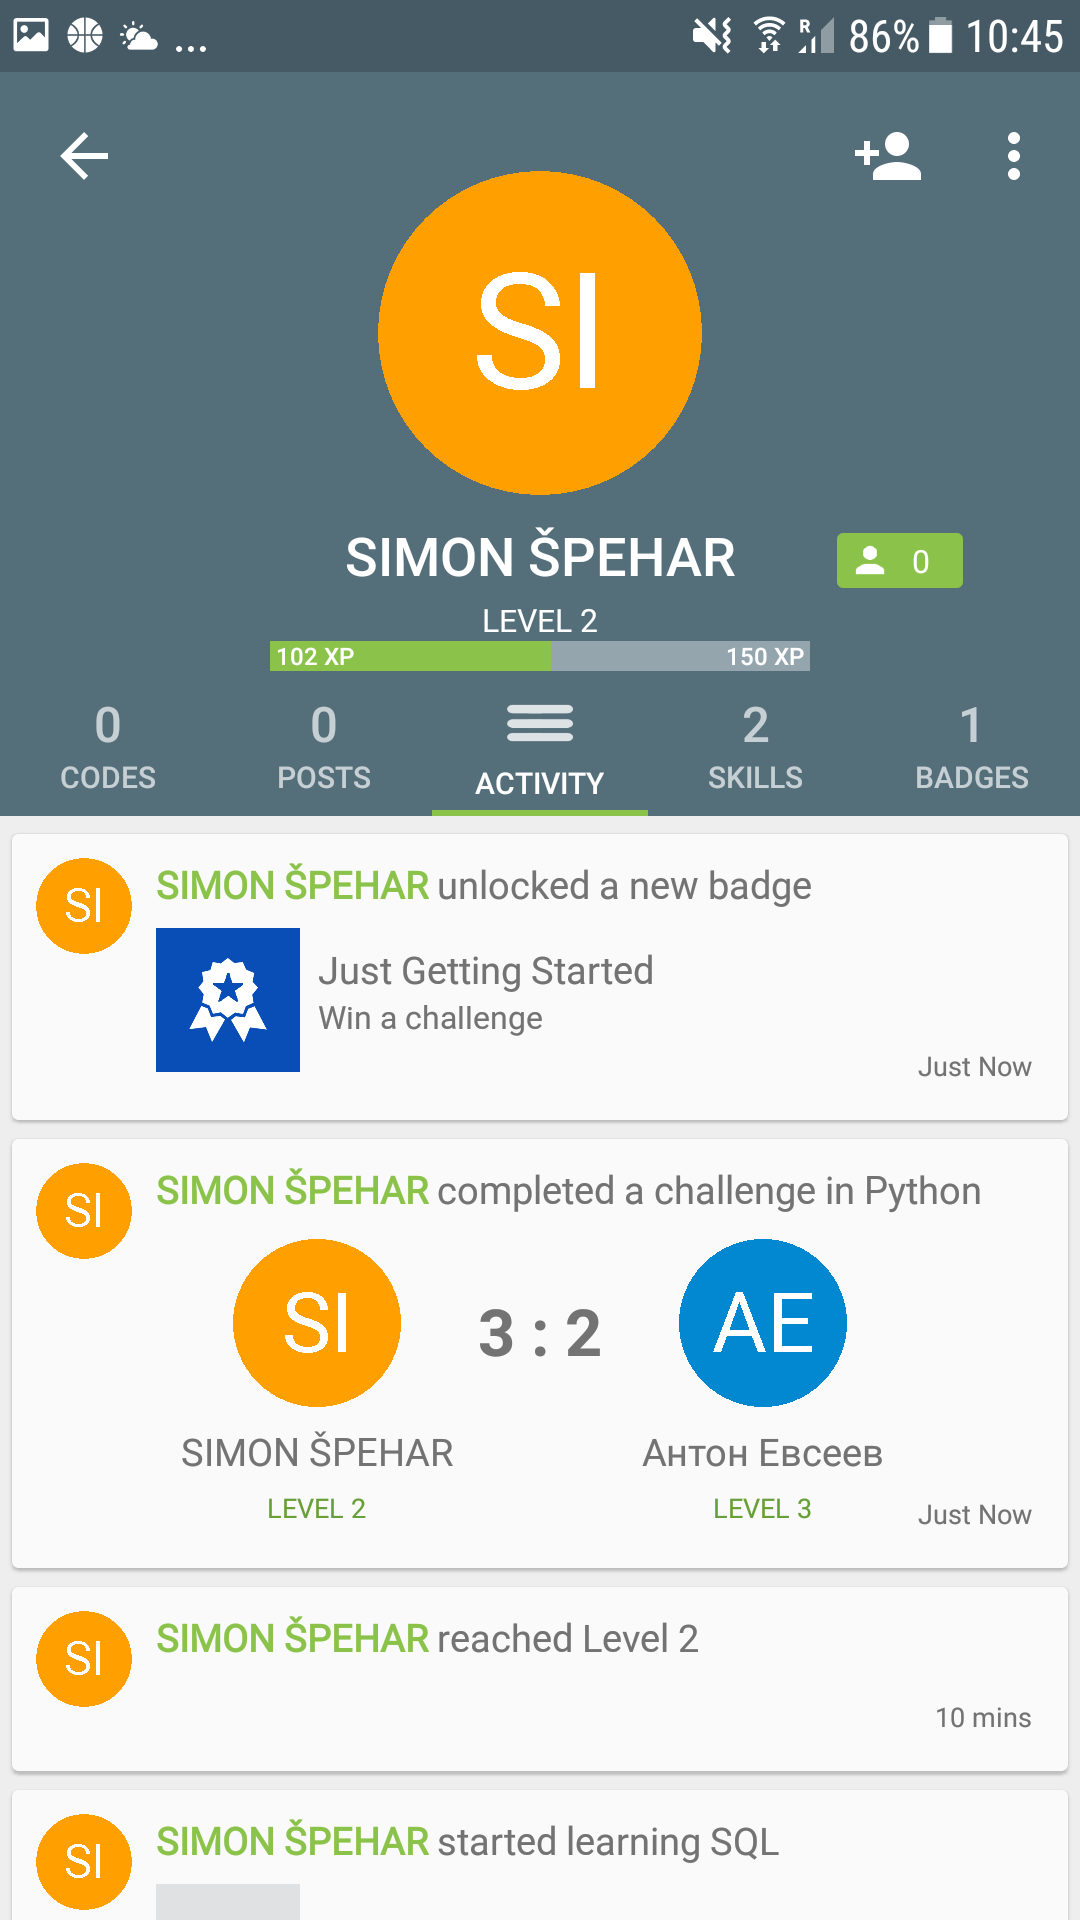
\includegraphics[height=0.7\textwidth]{slike/SoloLearn_person}
\caption{Področja programskega jezika Python}\label{sololearn}
\end{figure}
\noindent Lestvica v aplikaciji je razdeljena na globalno, v kateri so vsi uporabniki aplikacije, lokalno, ki vsebuje uporabnike, ki prihajajo iz širše okolice in lestvico prijateljev na kateri so vključeni uporabniki, ki so bili v aplikaciji dodani kot prijatelji.\\Aplikacija je dostopna na platformah Android in IOS, kot tudi preko spletnega brskalnika.
\chapter{Predstavitev spletne aplikacije}
Mobilno učenje je širok pojem, ki zajema vrsto aplikacij za različne namene. Nekatere so namenjene učenju jezikov, nekatere učenju zgodovine, matematike ali pa kuhanja. Mnoge od teh aplikacij uporabnike animirajo tudi z uporabo principov iger. Sami smo se odločili, da bodo uporabniki naše aplikacije spoznavali kraje, objekte in predmete, ki ne bodo omejeni na eno tematiko. S tem bodo uporabniki pridobili bolj splošno znanje iz različnih ved. Vsebina nalog bo tudi lokacija, katero bodo morali uporabniki obiskati, če bodo želeli sodelovati v igri. Del sistema, ki skrbi za vsebino nalog in preko katerega bo skrbnik sistema naloge urejal, bomo predstavili v tem poglavju.


Da bi lahko ustvarjali nove naloge za uporabnike, smo naredili spletni portal, ki omogoča, da se uporabnik avtenticira na strani in dodaja ali ureja vsebino izzivov. Preko enostavnega uporabniškega vmesnika je tako mogoče dodajati novo vsebino, kot tudi urejati že obstoječo.\\Poleg urejanja tekstovnih podatkov kot so, naslov, opis in točke izzivov, je mogoče urejati tudi lokacijo in predstavitveno sliko naloge. Za ta namen je bil vključen tudi zemljevid, na katerem uporabnik za posamezno nalogo enostavno označi kraj kjer bo ta aktivna.\\
Del spletne aplikacije je tudi aplikacijski programski vmesnik, ki omogoča prenos podatkov do mobilne aplikacije, kot tudi shranjevanje rezultatov v podatkovno bazo. Za te potrebe je bil razvit nov Laravel projekt, ki uporablja isto podatkovno bazo kot spletni portal. Ker smo želeli omejiti dostop do teh podatkov le na avtenticirane uporabnike,  smo uporabili avtentikacijo z žetoni. Slika~\ref{UML-Spletna} prikazuje diagram primerov uporabe spletne aplikacije.

\begin{figure}[H]
\centering
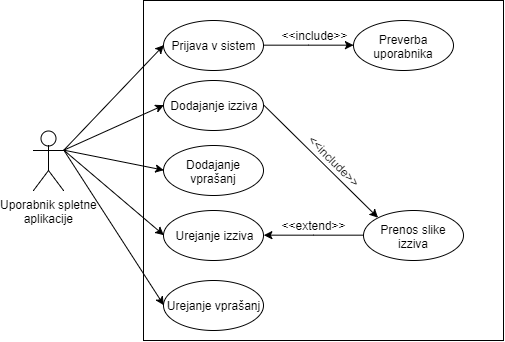
\includegraphics[height=0.65\textwidth]{slike/UML-Spletna}
\caption{Diagram primerov uporabe spletne aplikacije}\label{UML-Spletna}
\end{figure}
Za razvoj obeh aplikacij smo uporabili različico 5.4 Laravel ogrodja.\\V sledečih podpoglavjih bomo razložili delovanje posameznih komponent aplikacije, ter posebnosti pri razvoju.
\newpage
\section{Registracija spletnih virov}
Za delovanje Laravel aplikacije moramo, glede na storitev, definirati vire kamor lahko naslovimo uporabniške zahteve. V najenostavnejšem primeru so to preusmeritvene poti, ki omogočajo prehode med različnimi stranmi znotraj aplikacije, v bolj kompleksnejšem primeru pa so to naslovi, kamor  pošljemo zahtevo za pridobitev ali shranjevanje podatkov v bazo na REST način.

Vse spletne preusmeritve so potem, ko jih definiramo v datoteki \textit{web.php}, avtomatično na voljo za uporabo in lahko do njih dostopamo preko spletnega brskalnika ali REST klienta, kot je naprimer Postman~\cite{postman}. Namembna preusmeritev zahtevo sprejme in jo po potrebi posreduje naprej kontrolerju, ki je registriran na naslovu, ali pa sama izvede potrebno operacijo. Pri registraciji preusmeritve določimo, kakšno REST metodo pričakujemo. Poleg standardnih metod, kot so \textit{get, post, put}, lahko uporabimo tudi metodo \textit{resource}, vendar moramo v tem primeru v kontrolni logiki definirati funkcije z vnaprej določenim poimenovanjem. Datoteka, s preusmeritvami v spletni aplikaciji, poleg avtomatično dodanih virov za avtentikacijo, vsebuje tudi naslove za prikaz, urejanje ter brisanje izzivov in vprašanj vezanih na posamezen izziv. V vseh primerih preusmeritev, smo definirali kontrolerje in njihove funkcije, ki izvedejo potrebno akcijo. Slika~\ref{larawebroutes} prikazuje vsebino datoteke web.php, v kateri smo določili REST vire za različne akcije znotraj spletne aplikacije.
\begin{figure}[H]
\centering
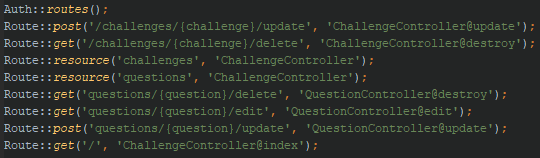
\includegraphics[height=0.3\textwidth]{slike/larawebroutes}
\caption{Definirane preusmeritve v spletnem portalu}\label{larawebroutes}
\end{figure}

\section{Kontrolerji}
Kontrolerji v Laravel, ali katerem koli drugem MVC ogrodju, implementirajo funkcije, ki se izvedejo kot posledica zahteve uporabnika oziroma sistema v pogledu aplikacije. Preden zahtevo obdelamo, ponavadi v njih preverimo, ali je bila zahteva avtenticirana. V Laravel ogrodju za avtentikacijo virov poskrbi vnaprej definiran \textit{auth} vmesnik, ki ga vključimo v konstruktorju posameznega kontrolerja. Vmesnik deluje tako, da za vsako zahtevo preveri ali je poslana s strani avtenticiranega uporabnika in, če ni, uporabnika preusmeri na prijavno stran. Spodnja koda prikazuje funkcijo, ki je definirana v kontrolerju in se uporablja, kadar želimo pridobiti seznam vseh izzivov za nekega uporabnika.
\begin{lstlisting}
public function getChallengesForUser($id)
{
    $player = Player::find($id);
    $challenges = DB::table('challenges')
        ->where('level', '<=', $player['level'])
        ->get();
    return response()->json(['data' => $challenges], 200);
}
\end{lstlisting}
Če je zahteva sprejeta s strani vmesnika, je posredovana naprej do funkcije, ki je bila registrirana na poklicanem viru v \textit{web.php}.\\Funkcije vsebujejo logiko za branje podatkov ali pisanje v bazo, ponavadi implementirano z Eloquent ORM, ali pa za preusmeritev na želeno stran znotraj aplikacije, včasih pa kar oboje.
\section{Prijavno okno}
Preko prijavnega okna se uporabnik avtenticira v spletno aplikacijo.\\Začetni koraki implementacije avtentikacije v uporabljenem ogrodju so enostavni. Preko ukazne vrstice v projektu izvršimo ukaz \textit{php artisan make:auth}, ki poskrbi za generiranje datotek za pogled, torej prijavnega okna, \textit{User} razreda v katerem definiramo lastnosti uporabnika, sheme podatkovne baze, ki vsebuje stolpce potrebne za shranjevanje uporabnikov, ter ostalih konfiguracijskih datotek in funkcij, ki jih uporabljamo pri upravljanju z uporabniki v naši aplikaciji~\cite{laraauth}.

Ko so vse datoteke pripravljene za uporabo, jih seveda prilagodimo našim potrebam. Nastaviti je potrebno, kam želimo, da nas aplikacija preusmeri po uspešni avtentikaciji. V datoteki \textit{LoginController}, ki skrbi za upravljanje prijavnih akcij, smo nastavili spremenljivko \texttt{\$redirectTo = '/challenges'}, ta poskrbi, da nas bo aplikacija preusmerila na vsebino, ki je dostopna preko vira \texttt{/challenges}, ki smo ga nastavili datoteki za spletne preusmeritve.\\Z zgornjim CLI ukazom se generirajo tudi datoteke namenjene za implementacijo registracije novih uporabnikov, vendar tega nismo uporabili, dostop je omogočen samo prednastavljenim uporabnikom.\\Spremenili smo tudi privzeti pogled prijavnega okna, kot to prikazuje slika~\ref{portal_login}.
\begin{figure}[H]
\centering
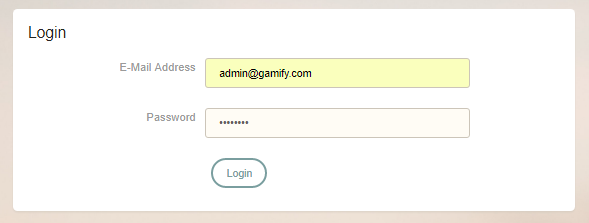
\includegraphics[height=0.4\textwidth]{slike/portal_login}
\caption{Prijavno okno}\label{portal_login}
\end{figure}
\newpage
\section{Prikaz izzivov}
Po uspešni avtentikaciji smo preusmerjeni na stran za prikaz izzivov. Ti so prikazani v seznamu razvrščenem po času nastanka. Uporabniku prikažemo naslov, kratek opis, število točk ter stopnjo naloge. Od tukaj lahko izzive brišemo, ali pa s klikom na naslov odpremo stran za urejanje.

V kontrolerju \texttt{ChallengeController}, smo definirali funkcijo \texttt{index()}, kot jo prikazuje spodnja koda, ki iz baze pridobi podatke o vseh izzivih, ter s pridobljenimi podatki prikaže nov pogled.
\begin{lstlisting}[label=lst:index]
public function index()
    {
        $challenges = Challenge::latest()->get();
        return view('challenges.index', compact('challenges'));
    }
\end{lstlisting}
Spremenljivka \texttt{challenges}, ki smo jo definirali v kontrolerju, je nato na voljo v pogledu, zato lahko z zanko enostavno izpišemo vse podatke.\\Del ogrodja so Blade predloge~\cite{larablade}, s katerimi lahko upravljamo izpis v pogledu, vključujemo druge Blade predloge, določamo sekcije, ali pa v zanki izpišemo vrednosti določene spremenljivke. Vse Blade predloge so pred uporabo prevedene v PHP jezik.\\Laravel ponuja tudi veliko vnaprej razvitih funkcij kot je naprimer \texttt{diffFOrHumans()}, ki časovni zapis iz podatkovne baze, pretvori v prijaznejšo obliko.\\Koda, ki sledi, prikazuje uporabo Blade predlog in PHP spremenljivk znotraj HTML dokumenta.
\bigskip
\begin{lstlisting}
@foreach($challenges as $challenge)
    <tr>
        <td><a href="{{$challenge->path()}}/edit">
            <h4>{{$challenge->title}}</a></h4>
            <small>{{$challenge->created_at->diffFOrHumans()}}</small>   
        </td>
        <td>{{ str_limit($challenge->description, 120, '...')}}</td>
        <td>{{$challenge->points}}</td>
        <td>{{$challenge->level}}</td>
        <td><a href="{{$challenge->path()}}/delete">
        <i class="material-icons">delete</i></a></td>
    </tr>
@endforeach
\end{lstlisting}
Koda uporablja zanko za izpis vseh vnosov, ki so v tabeli izzivov. Podatke izzivov na uporabniškem vmesniku predstavimo tako kot prikazuje slika~\ref{portal_index}.
\begin{figure}[H]
\centering
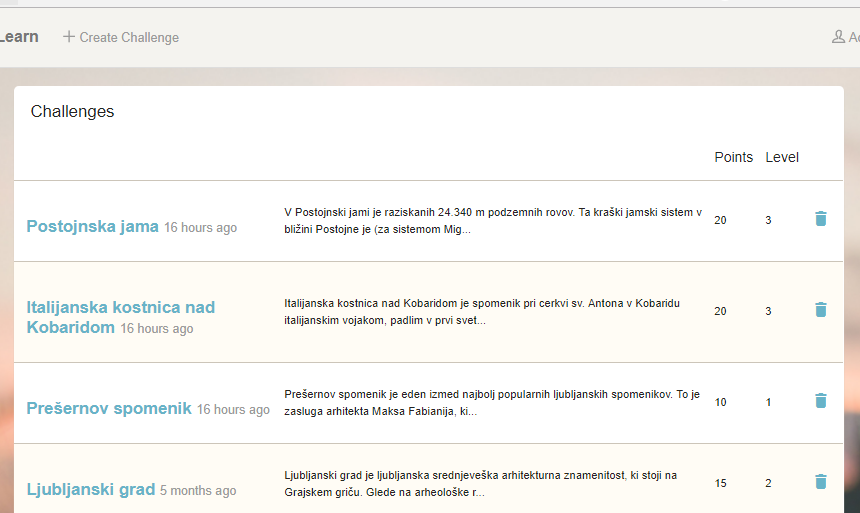
\includegraphics[height=0.6\textwidth]{slike/portal_index}
\caption{Prva stran portala s seznamom izzivov}\label{portal_index}
\end{figure}
\label{ch6}
\section{Dodajanje novih izzivov}
Naredili smo enostaven uporabniški vmesnik za dodajanje novih nalog uporabnikom. Vnesemo lahko naslov izziva, ki bo ponavadi povezan s krajem, kjer se izziv izvaja, vrednost izziva v točkah, stopnjo, ki določa kateri uporabniki bodo lahko izziv videli, kratek opis, lokacijo ter sliko, ki bo prikazana v mobilni aplikaciji ob nalogi.

Ko izpolnemo vsa polja in shranimo nov izziv, se ustvari zahteva, ki preko vira definiranega kot \texttt{Route::resource('challenges', 'ChallengeController');} prispe do funkcije \texttt{store(Request \$request)} v \texttt{ChallengeController} kontrolerju. Funkcija iz zahteve prebere sliko, ustvari novo ime, ter jo shrani na strežnik. Pravtako iz zahteve prebere vrednosti vseh definirani polj, ki jih je uporabnik izpolnil v pogledu in ustvari nov zapis v podatkovni bazi.\\Naslednja koda predstavlja funkcijo \texttt{store}, ki se uporablja za zgoraj omenjeni postopek shranjevanja zapisov v bazo. 

\begin{lstlisting}
public function store(Request $request)
{
    $photo = $request->file('photo');
    $name = time() . $photo->getClientOriginalName();
    $photo->move('images/photos', $name);
    $challenge = Challenge::create(
        ['title' => $request->title,
        'points' => $request->points,
        'location' => $request->location,
        'geojson' => $request->geojson,
        'description' => $request->description,
        'level' => $request->level,
        'photo' => $name
        ]);   
    return redirect('/challenges/' . $challenge->id . '/edit');
}
\end{lstlisting}

\noindent V tem trenutku uporabnik še ne definira lokacije naloge, ki se nahaja v polju \texttt{geojson}. V to polje ob kreiranju novega izziva zapišemo neko privzeto vrednost in nato uporabnika preusmerimo na stran za urejanje, kjer lahko na zemljevidu označi lokacijo kjer bo naloga aktivna.
\section{Urejanje vsebine izzivov}
Vsakemu posameznemu izzivu lahko posodobimo opis, naslov, točke, stopnjo, sliko in tudi lokacijo na zemljevidu. V pogledu urejanja lahko dostopamo tudi do pogleda za dodajanje ali urejanje vprašanj izziva.\\Vključen je zemljevid Google Maps, na katerem smo razvili možnost označbe lokacije, kjer bo uporabnikom mobilne aplikacije izziv na voljo. Izbirno polje lahko poljubno povečamo ali pomanjšamo, ter ga tudi premikamo po zemljevidu. S tem spreminjamo koordinate lika, ki jih ob posodobitvi pretvorimo v json obliko in shranimo v bazo. Kadar jih želimo prebrati iz baze, jih pretvorimo nazaj v objekt \texttt{LatLngBounds}, ki vsebuje funkcijo \texttt{contains()}, s katero lahko preverimo, če je trenutna lokacija uporabnika znotraj označene lokacije na zemljevidu.\\Funkcijo \texttt{serialize}, ki je prikazana v sledeči kodi, uporabimo za pretvorbo koordinat naprave v json obliko, preden jih shranimo v bazo. 
\begin{lstlisting}
function serialize() {
    var json = '{"bounds":' + rectangle.getBounds().toString()+'}';
    json = json.replace(/\(/g, "[").replace(/\)/g, "]");
    return json;
}
\end{lstlisting}
Funkcijo \texttt{deserialize} uporabimo za pretvorbo json koordinat v LatLngBounds objekt, kot prikazuje spodnja koda.
\begin{lstlisting}
function deserialize(json) {
    json = JSON.parse(json.value);
    return new google.maps.LatLngBounds(
    	new google.maps.LatLng(json.bounds[0][0], json.bounds[0][1]),
    	new google.maps.LatLng(json.bounds[1][0], json.bounds[1][1])
    );
}
\end{lstlisting}
\newpage
\noindent Pogled, ki omogoča spreminjanje lokacije posameznega izziva na zemljevidu, je prikazan na sliki~\ref{gmaps}.
\begin{figure}[H]
\centering
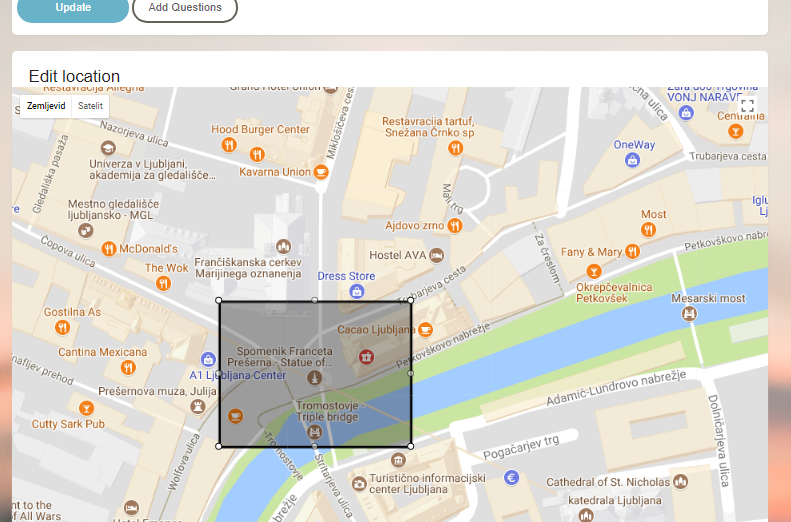
\includegraphics[height=0.65\textwidth]{slike/gmaps}
\caption{Izbira lokacije izziva na zemljevidu Google Maps}\label{gmaps}
\end{figure}

\section{Dodajanje vprašanj k izzivom}
Vsak izziv lahko vsebuje več vprašanj na katere uporabniki mobilne aplikacije odgovarjajo in s tem pridobivajo točke.\\Podobno kot pri samem izzivu, moramu tudi vprašanjem določiti vrednost v točkah ter stopnjo, ki pove, igralci katere stopnje lahko odgovorijo na vprašanje.

Ker uporabljamo objektno relacijsko preslikovanje, smo v razredih \texttt{Challenge} in \texttt{Question} definirali funkcije, ki opišejo povezavo med entitetama, da je med njima možno mapiranje vnosov na način ena proti mnogo. Označiti moramo, da vprašanja pripadajo izzivom. To smo storili v razredu \texttt{Question}, kjer smo za ta namen uporabili funkcijo \texttt{belongsTo}.\\Opisano prikazuje naslednja koda.

\begin{lstlisting}
class Question extends Model
{
    public function challenge()
    {
        return $this->belongsTo(Challenge::class);
    }
}
\end{lstlisting}
V modelu za izzive, pa smo definirali možnost večih vnosov v tabelo \texttt{questions}, ki so preko tujega ključa povezane s tabelo \texttt{challenges}. Napisali smo tudi funkcijo, ki jo pokličemo iz kontrolerja, kadar izzivu želimo dodati novo vprašanje. Spodnja koda opisuje kako na objektu določiti povezavo ena proti mnogo in kako preko funkcije \texttt{addQuestion} dodamo vprašanje k izzivu. Uporabili smo Eloquent funkciji \texttt{hasMany} ter \texttt{create}
\begin{lstlisting}
public function questions()
{
    return $this->hasMany(Question::class);
}
public function addQuestion($reply)
{
    $this->questions()->create($reply);
}
\end{lstlisting}

Vsakemu vprašanju, ki ga ustvarimo, moramo dodati štiri možne odgovore. Izberemo tudi pravilni odgovor, ki se zapiše skupaj z vprašanjem v bazo. Tako lahko v mobilni aplikaciji enostavno preverimo točnost odgovora.\\V samem pogledu imamo tudi seznam vseh vprašanj, katere lahko s klikom na vprašanje urejamo, ali pa jih pobrišemo s klikom na ikono koša.\\Slika~\ref{questions} prikazuje uporabniški vmesnik za dodajanje novih vprašanj oziroma urejanje obstoječih. Do tega pogleda dostopamo iz pogleda za urejanje izzivov.
\begin{figure}[H]
\centering
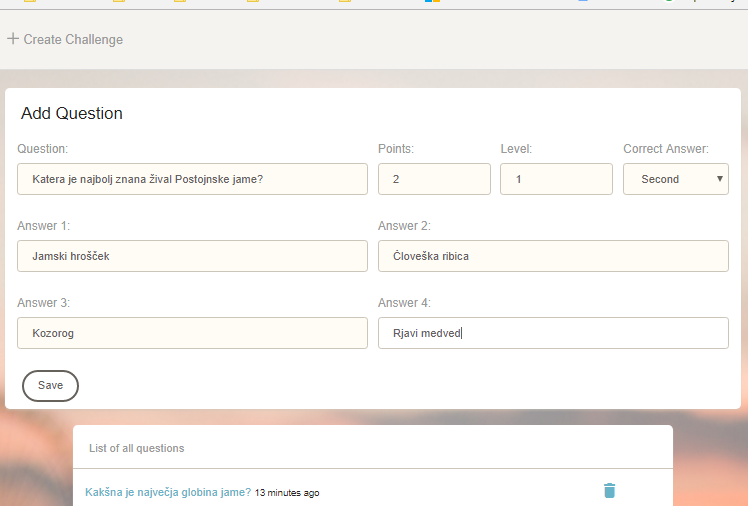
\includegraphics[height=0.66\textwidth]{slike/questions}
\caption{Ustvarjanje novega vprašanja z odgovori.}\label{questions}
\end{figure}

\section{REST API strežnik}
Posebno aplikacijo namenjeno komunikaciji mobilne aplikacije z bazo, v kateri so shranjeni podatki o uporabnikih in izzivi, smo pravtako napisali s pomočjo Laravel ogrodja. Nadgradili smo jo s paketom Dingo API, ki je posebej namenjen izdelavi Laravel REST aplikacij~\cite{Dingo}. Omogoča verzioniranje REST virov, paginacijo, upravljanje z napakami in avtentikacijo virov. Tudi te REST vire definiramo v datoteki \texttt{web.php}.

Implementirali smo različne funkcije, ki omogočajo delovanje mobilne aplikacije. Zahteve, ki pridejo s strani mobilne aplikacije so preverjene, če imajo veljaven žeton, nato pa posredovane registriranim funkcijam v kontrolerju. Slika~\ref{REST_communication} prikazuje potek komunikacije mobilne aplikacije s strežnikom, ko uporabnik uporablja pogled s seznamom izzivov. 
\begin{figure}[H]
\centering
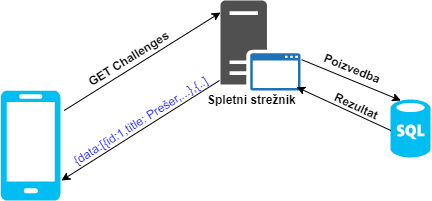
\includegraphics[height=0.35\textwidth]{slike/REST}
\caption{Potek zahteve mobilne aplikacije za seznam izzivov.}\label{REST_communication}
\end{figure}
\noindent V primeru, če žeton ni veljaven, torej uporabnik ni avtenticiran, je v JSON odgovoru shranjena napaka, kar omogoča nadaljnje rokovanje mobilne aplikacije. V nasprotnem primeru je v odgovoru shranjen rezultat poizvedbe, ki ga prikažemo v mobilni aplikaciji. Spodnja koda opisuje funkcijo, ki se uporablja za pridobitev izzivov posameznega uporabnika. Funkcija vrne samo izzive, ki imajo definirano stopnjo manjšo ali enako kot jo ima igralec trenutno.
\bigskip
\begin{lstlisting}
public function getChallengesForUser($id)
{
    $player = Player::find($id);
    $challenges = DB::table('challenges')
        ->where('level', '<=', $player['level'])
        ->get();
    return response()->json(['data' => $challenges], 200);
}
\end{lstlisting}
\subsection{JWT avtentikacija}
\label{6:jwt}
Avtentikacija z žetoni, bolj znana pod imenom JWT~\cite{jwt} oziroma Json Web Tokens, je način varnega prenašanja json vsebine, preko nezavarovane povezave kot je naprimer http. Omogoča nam, da uporabnikom, ki niso avtenticirani, preprečimo branje ali pisanje v podatkovno bazo.

Avtentikacija uporabnika na strežniku ustvari nov žeton, ki ga v odgovoru na zahtevo po avtentikaciji, strežnik vrne klientu. Vsaka zahteva klienta, ki sledi, mora v glavi zahteve ali pa v URL poizvedbi vsebovati dotični žeton. Če žeton ne obstaja, ali pa je njegova veljavnost potekla, strežnik klientu v odgovoru pošlje izjemo, ki jo lahko nato pravilno obravnavamo v izvorni kodi klienta. Za implementacijo JWT smo uporabili odprtokodno knjižnico \texttt{jwt-auth}~\cite{tymon}, za katero ima Dingo paket, ki smo ga uporabili za razvoj REST virov, vgrajeno podporo. Spodnja koda prikazuje način rokovanja prijave uporabnika kot smo ga opisali zgoraj.
\begin{lstlisting}
public function authenticate(Request $request)
    {
        $credentials = $request->only('username', 'password');
        $token = JWTAuth::attempt($credentials);
        try {
            if (!$token = JWTAuth::attempt($credentials)) {
                return response()->json(['error' => 'User credentials invalid'], 401);
            }
        } catch (JWTException $e) {
            return "error";
        }
        return response()->json(compact('token'))->setStatusCode(200);
    }
\end{lstlisting}
V kontrolerju REST aplikacije, smo implementirali \texttt{authenticate} funkcijo, ki je potrebna za generiranje žetona po uspešni avtentikaciji uporabnika. Iz zahteve izluščimo uporabniško ime in geslo, ter ju poskušamo overiti preko vmesnika, ki ga ponuja knjižnica.\\V konfiguracijski datoteki nastavimo uporabniški model, ki ga knjižnica uporabi za avtentikacijo, v primeru api strežnika smo nastavili model \texttt{Player}, ki predstavlja tabelo \texttt{players} v podatkovni bazi.\\ Ob uspešnem overjanju, klientu vrnemo json odgovor z novim žetonom, v nasprotnem primeru, pa avtentikacijo zavrnemo.\\Koda, ki sledi, se uporablja po uspešni avtentikaciji za poizvedbo podatkov vpisanega uporabnika. Kadar poizvedba ni uspešna, v odgovoru na zahtevo pošljemo primerno sporočilo.
\begin{lstlisting}
public function getAuthenticatedUser()
    {
        try {
            if (! $user = JWTAuth::parseToken()->authenticate()) {
                return response()->json(['user_not_found'], 404);
            }
        } catch (Exception\TokenExpiredException $e) {
            return response()->json(['token_expired'], $e->getStatusCode());
        } catch (Exception\TokenInvalidException $e) {
            return response()->json(['token_invalid'], $e->getStatusCode());
        } catch (JWTException $e) {
            return response()->json(['token_absent'], $e->getStatusCode());
        }
        return response()->json(compact('user'));
    }
\end{lstlisting}
Ob klicu funkcije \texttt{getAuthenticatedUser()} moramo zahtevi dodati prej pridobljen žeton.
\chapter{Predstavitev mobilne aplikacije}
\label{ch7}
Mobilno učenje smo realizirali z Android mobilno aplikacijo razvito z ogrodjem Ionic, ki omogoča uporabnikom dinamično učenje novih vsebin preko igre. V razvoj smo vključili elemente gamifikacije kot so točke, pasica napredka, stopnje in lestvica. Kot smo opisovali v poglavju~\ref{2.1}, je kontekst pomemben del mobilnega učenja. Zato smo želeli pri uporabi aplikacije vključiti senzorje, ki lahko pripomorejo k boljši umestitvi učenja v kontekst okolice uporabnika. Razvili smo lokacijsko usmerjeno mobilno aplikacijo, v kateri so določene vsebine dostopne samo v definiranih območjih. S tem želimo uporabnike motivirati, da raziskujejo kraje in si iz prve roke ogledajo predmete učenja. Tako tudi samo učenje postavimo v kontekst z okolico. Ob vsakem obisku novega izziva uporabnik prejme točke, ki se seštevajo in uporabljajo za primerjavo z ostalimi igralci. Vsak izziv vsebuje povzetek dotičnega predmeta učenja in vprašanja, za katera uporabnik ob pravilnem odgovoru prejme točke.\\Aplikacija preko avtenticiranih REST klicev dostopa do podatkov, ustvarjenih na spletnem portalu, na enak način tudi shranjuje informacije o napredku uporabnikov. Poleg prijave obstoječih uporabnikov v sistem, se lahko registrirajo tudi novi uporabniki.
\newpage
\noindent Znotraj same aplikacije smo razvili več pogledov, kot so naprimer pogled za pregled trenutnih rezultatov, seznam izzivov, ki jih igralec lahko opravi, opis predmeta učenja, vprašanja, ter pogled lestvice, kjer se lahko uporabnik primerja z ostalimi igralci. Slika~\ref{UML-mobilna} prikazuje diagram primerov uporabe mobilne aplikacije.
\begin{figure}[H]
\centering
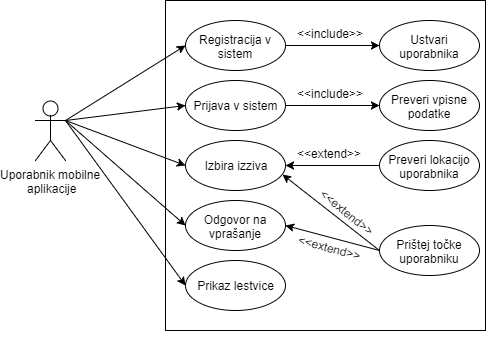
\includegraphics[height=0.65\textwidth]{slike/UML-mobilna}
\caption{Diagram primerov uporabe mobilne aplikacije. }\label{UML-mobilna}
\end{figure}

V nadaljevanju bomo podrobneje opisali vse dele mobilne aplikacije, ter potek razvoja.
\section{Avtentikacija}
Preden lahko uporabnik dostopa do vsebine, mora prejeti avtentikacijski ključ, ki ga uporablja tekom procesa pridobivanja ali pisanja podatkov. Ključ prejme po uspešni avtentikaciji preko prijavnega okna kot ga vidimo na sliki~\ref{mobile_login}.
\begin{figure}[H]
\centering
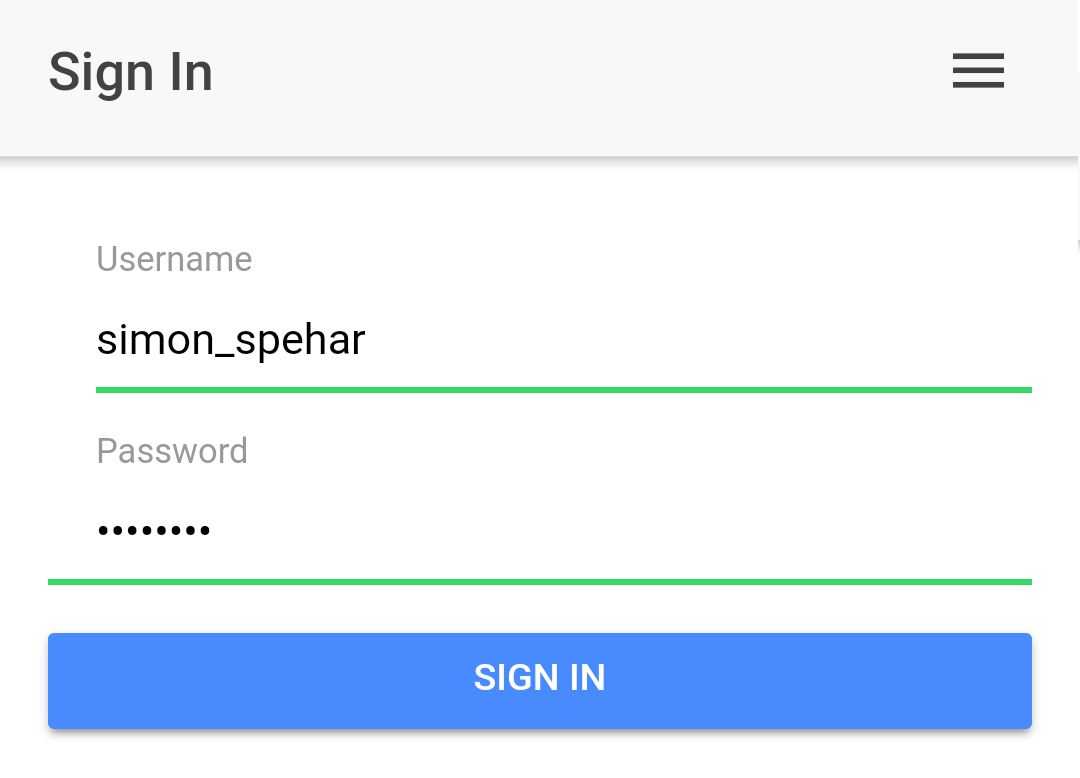
\includegraphics[height=0.45\textwidth]{slike/mobile_login}
\caption{Prijavno okno.}\label{mobile_login}
\end{figure}
\noindent Preko REST klica posredujemo uporabniško ime in geslo na strežnik, ki zahtevo preveri kot je opisano v poglavju \ref{6:jwt} in nato ustrezno odgovori. V primeru neuspešne avtentikacije uporabniku prikažemo sporočilo o napačnem uporabniškem imenu ali geslu. Če je avtentikacija uspela, pa prejeti ključ shranimo lokalno v aplikaciji in ga uporabljamo za vse nadaljnje klice, dokler ta ne poteče, ali pa se uporabnik odjavi iz sistema. Funkcija \texttt{signin} v mobilni aplikaciji, ki je namenjena avtentikaciji uporabnikov, je prikazana spodaj.
\begin{lstlisting}
public signin(username: string, password: string) {
    return this.http.post('http://api.spehar.si/api/authenticate', {username, password})
        .map(res=>res.json());
}
\end{lstlisting}
\bigskip
Prvi klic, ki ga aplikacija avtomatično naredi, ko je uporabnik prijavljen v sistem, opravi funkcija \texttt{getUser}, ki s strežnika v json obliki pridobi vse podatke o uporabniku. Ti podatki nato služijo prikazu uporabniškega vmesnika.
\section{Registracija novih uporabnikov}
Ob prvi uporabi aplikacije, se mora uporabnik registrirati v sistemu, kar pomeni, da mora izbrati uporabniško ime in geslo za prijavo. Registracija je ustvarjena, podobno kot prijava, preko REST klica na API strežnik.\\Uporaba obstoječih uporabniških imen ni mogoča, v tem primeru je izpisano primerno obvestilo. Pri vpisu gesla uporabljamo dva polja, ki preverjata, če se ni uporabnik pri izbiri gesla zatipkal. Dokler drugo polje ni izpolnjeno je gumb za registracijo onemogočen, kar lahko vidimo na sliki okna za registracijo uporabnika~\ref{mobile_register}.
\begin{figure}[H]
\centering
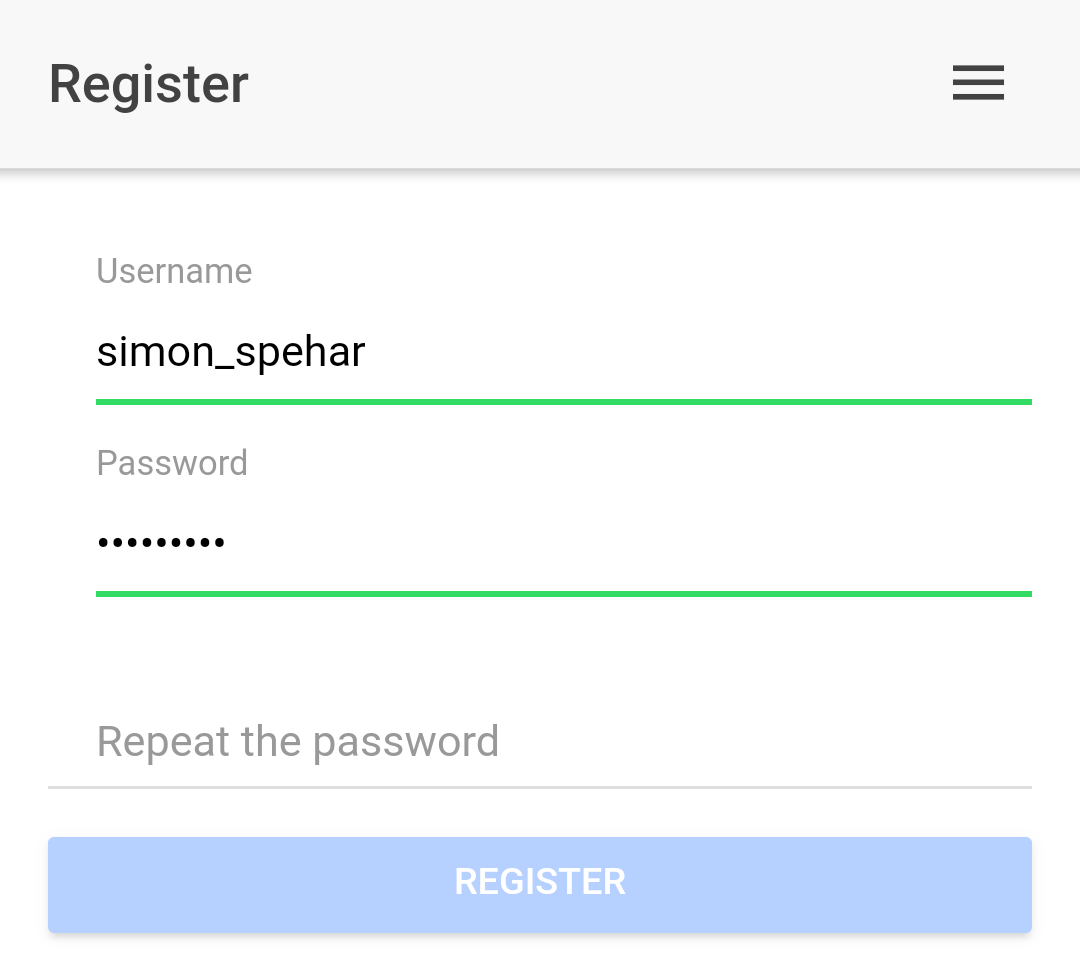
\includegraphics[height=0.55\textwidth]{slike/mobile_register}
\caption{Okno za registracijo novih uporabnikov.}\label{mobile_register}
\end{figure}
\noindent Kadar je registracija uspešna, je uporabnik preusmerjen na okno za vpis, od koder se lahko s svojim novim uporabniškim imenom in geslom avtenticira. 
\section{Pregled aktivnosti uporabnika}
Po prijavi v sistem, je uporabnik preusmerjen na prvo stran, kjer mu prikažemo njegovo trenutno stopnjo in pasico napredka v trenutni stopnji. Odločili smo se, da za imena stopenj, namesto številk uporabimo različna poimenovanja. Tako je naprimer prva stopnja \textit{Beginner}, naslednja \textit{Search worm} itd.\\Pravtako uporabniku prikažemo skupno število točk, ter koliko izzivov je opravil, oziroma na koliko vprašanj je odgovoril. Celotno stran pogleda aktivnosti uporabnika vidimo na sliki~\ref{profile}.
\begin{figure}[H]
\centering
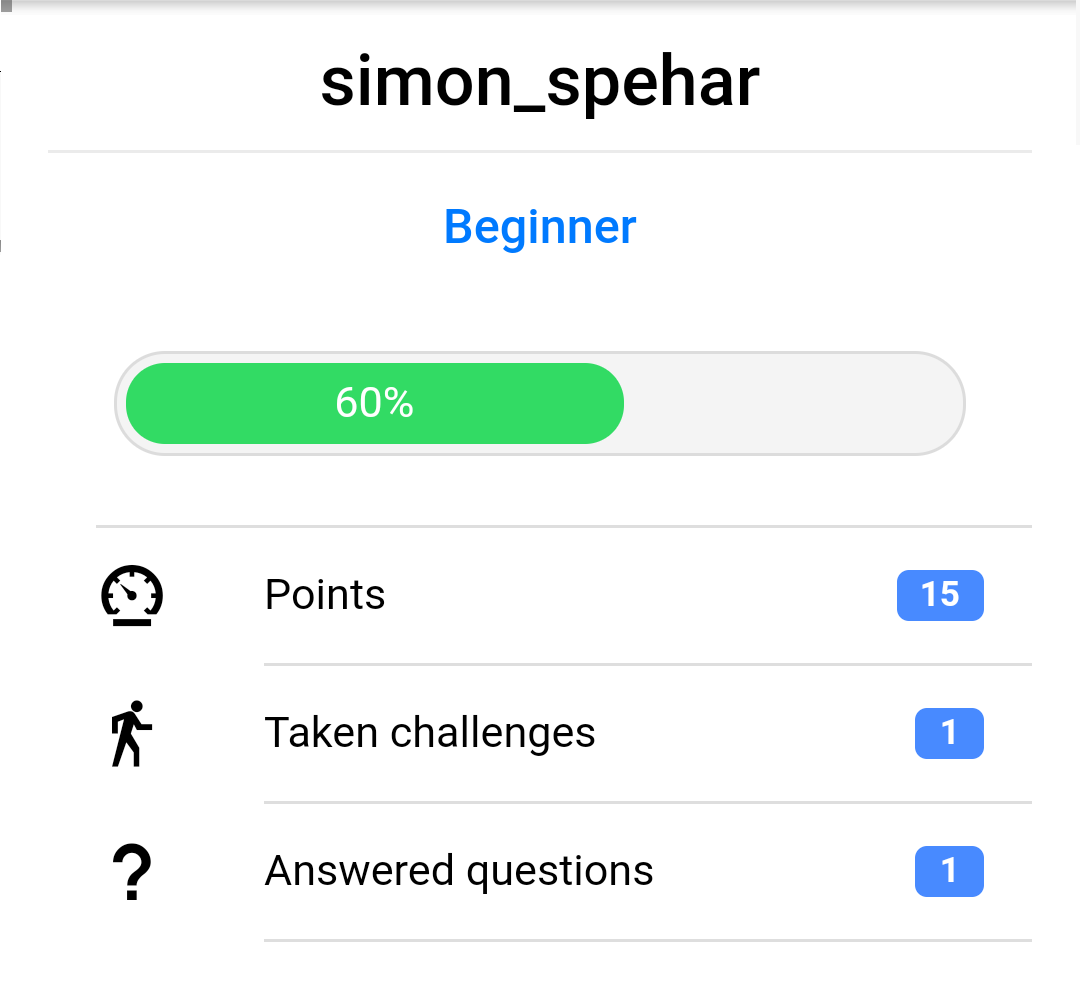
\includegraphics[height=0.5\textwidth]{slike/profile}
\caption{Uporabniška stran z aktivnostmi.}\label{profile}
\end{figure}

\noindent Vsaki stopnji smo določili število točk, ki jih uporabnik potrebuje za prehod v neko stopnjo. Vsakič, ko se ob aktivnosti uporabnika število točk posodobi, v izvorni kodi preverimo ali lahko uporabnik, na podlagi novega števila točk, preide v višjo stopnjo. Kadar želimo uporabniku povišati stopnjo, pokličemo funkcijo v naslednjem primeru kode.
\begin{lstlisting}
levelUp(userId, token) {
        return this.http.post("http://api.spehar.si/api/levelUp/" + userId + "?token=" + token)
            .map(res => res.json());
    }
\end{lstlisting}
V primeru, ko moramo uporabniku posodobiti stopnjo, to naredimo z REST klicem, ki v podatkovni bazi posodobi podatke in v odgovoru na zahtevo vrne uporabnika s posodobljenimi podatki. Ker lahko igralec tudi izgubi točke, če napačno odgovori na vprašanje, smo napisali tudi funkcijo, ki uporabniku zmanjša stopnjo, če je to potrebno.

\section{Seznam izzivov}
V pogledu seznama izzivov uporabniku prikažemo vse naloge oziroma izzive, ki so mu na voljo glede na njegovo trenutno stopnjo. Prikazani so izzivi, ki imajo določeno nižjo ali enako stopnjo, kot jo ima igralec sam. V izvorni kodi Ionic aplikacije, za vse strani, uporabljamo funkcijo \texttt{ionViewWillEnter()}, ki se izvede, preden je uporabnik preusmerjen na neko stran. V primeru pogleda seznama izzivov, v funkciji iz strežnika, poleg vseh izzivov, pridobimo tudi identifikatorje nalog, ki jih je uporabnik že opravil, tako vemo za katere naloge ne smemo uporabniku ponovno pripisati točk.\\
Da lahko igralec izziv odpre in za to pridobi točke, se mora nahajati na območju, ki je bilo določeno v spletni aplikaciji pri dodajanju ali urejanju naloge. Koda, ki sledi, prikazuje funkcijo \texttt{onLoadChallenge}, ki je poklicana kadar uporabnik poskuša dostopati do posameznega izziva. Njena naloga je, da ugotovi, če uporabnik lahko dostopa do izziva in, ali za izziv prejme točke.
\begin{lstlisting}
    onLoadChallenge(challenge, index) {
        this.geolocation.getCurrentPosition().then((data) => {
            if (this.contains(data.coords, challenge.geojson) || this.challengeTaken(challenge.id)) {
                if (!this.challengeTaken(challenge.id)) {
                    let toast = this.toastCtrl.create({
                        message: 'Good job!\nCollected ' + challenge.points + ' points',
                        duration: 3000,
                        position: 'bottom'
                    });
                    this.chService.collectChallenge(challenge.id, localStorage.getItem('userId'), localStorage.getItem('token')).subscribe(
                        (response) => {
                            toast.present();
                        });
                }
                this.navCtrl.push(ChallengePage, {challenge: challenge, index: index});
            } else {
                this.handleError("Where are you?", "You're not on challenge location");
            }
        });
    }
\end{lstlisting}
\noindent Kadar igralec ni v območju naloge in preko gumba \texttt{Open} poskusi izziv odpreti, v aplikaciji prikažemo opozorilo kot ga vidimo na sliki~\ref{where}. To ne velja, kadar je bil izziv že opravljen v preteklosti, v tem primeru je uporabnik preusmerjen na nalogo in lahko odgovarja na vprašanja, tudi, če ni na samem kraju izziva. 
\begin{figure}[H]
\centering
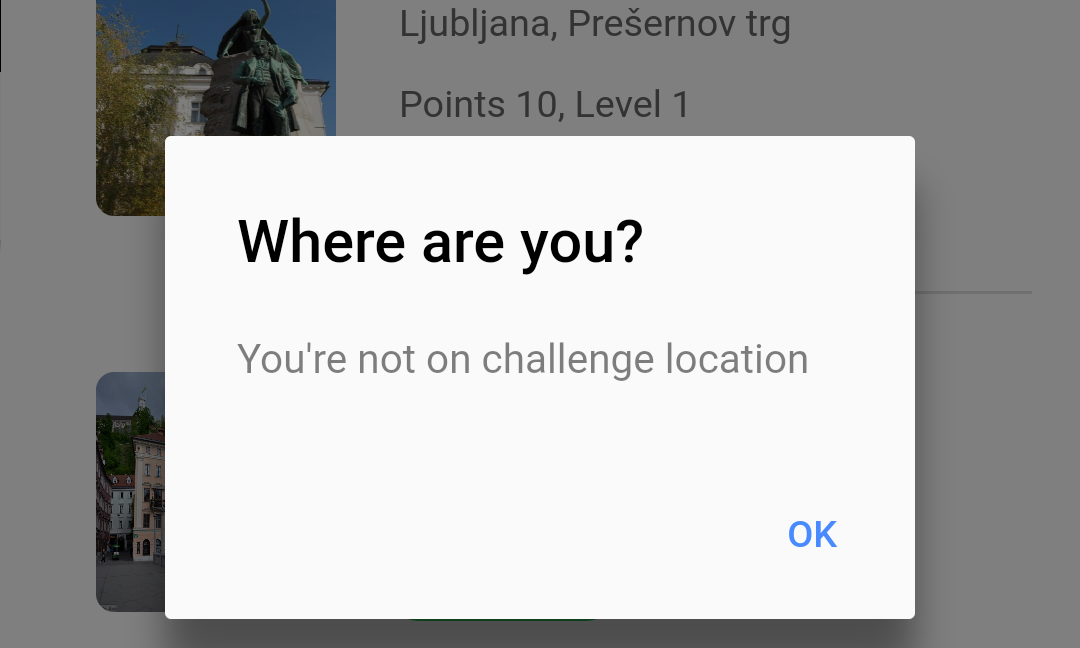
\includegraphics[height=0.4\textwidth]{slike/where}
\caption{Opozorilo o lokaciji uporabnika.}\label{where}
\end{figure}
\noindent V izvorni kodi lokacijo preverimo tako, da uporabimo funkcijo \texttt{contains}, ki ji podamo trenutne koordinate igralca ter mejne koordinate izbranega izziva. Če lokacija ustreza, preverimo še, če je uporabnik izziv že opravil in v nasprotnem primeru uporabniku prištejemo točke izziva, ter ga preusmerimo na sam izziv.\\V posamezenem elementu seznama, poleg naslova, dodamo sliko, ki prikazuje kraj ali predmet naloge, ter lokacijo in vrednost izziva v točkah. Izzive, ki jih je uporabnik že obiskal poznamo, saj v seznamu hranimo identifikatorje le teh in jih označimo s kljukico ob naslovu. Implementirali smo tudi osveževanje podatkov. Uporabniki lahko enostavno s potegom navzdol po zaslonu mobilne naprave osvežijo obstoječe podatke ali naložijo morebitne nove. Pogled seznama izzivov je prikazan na sliki~\ref{izzivi}.
\begin{figure}[H]
\centering
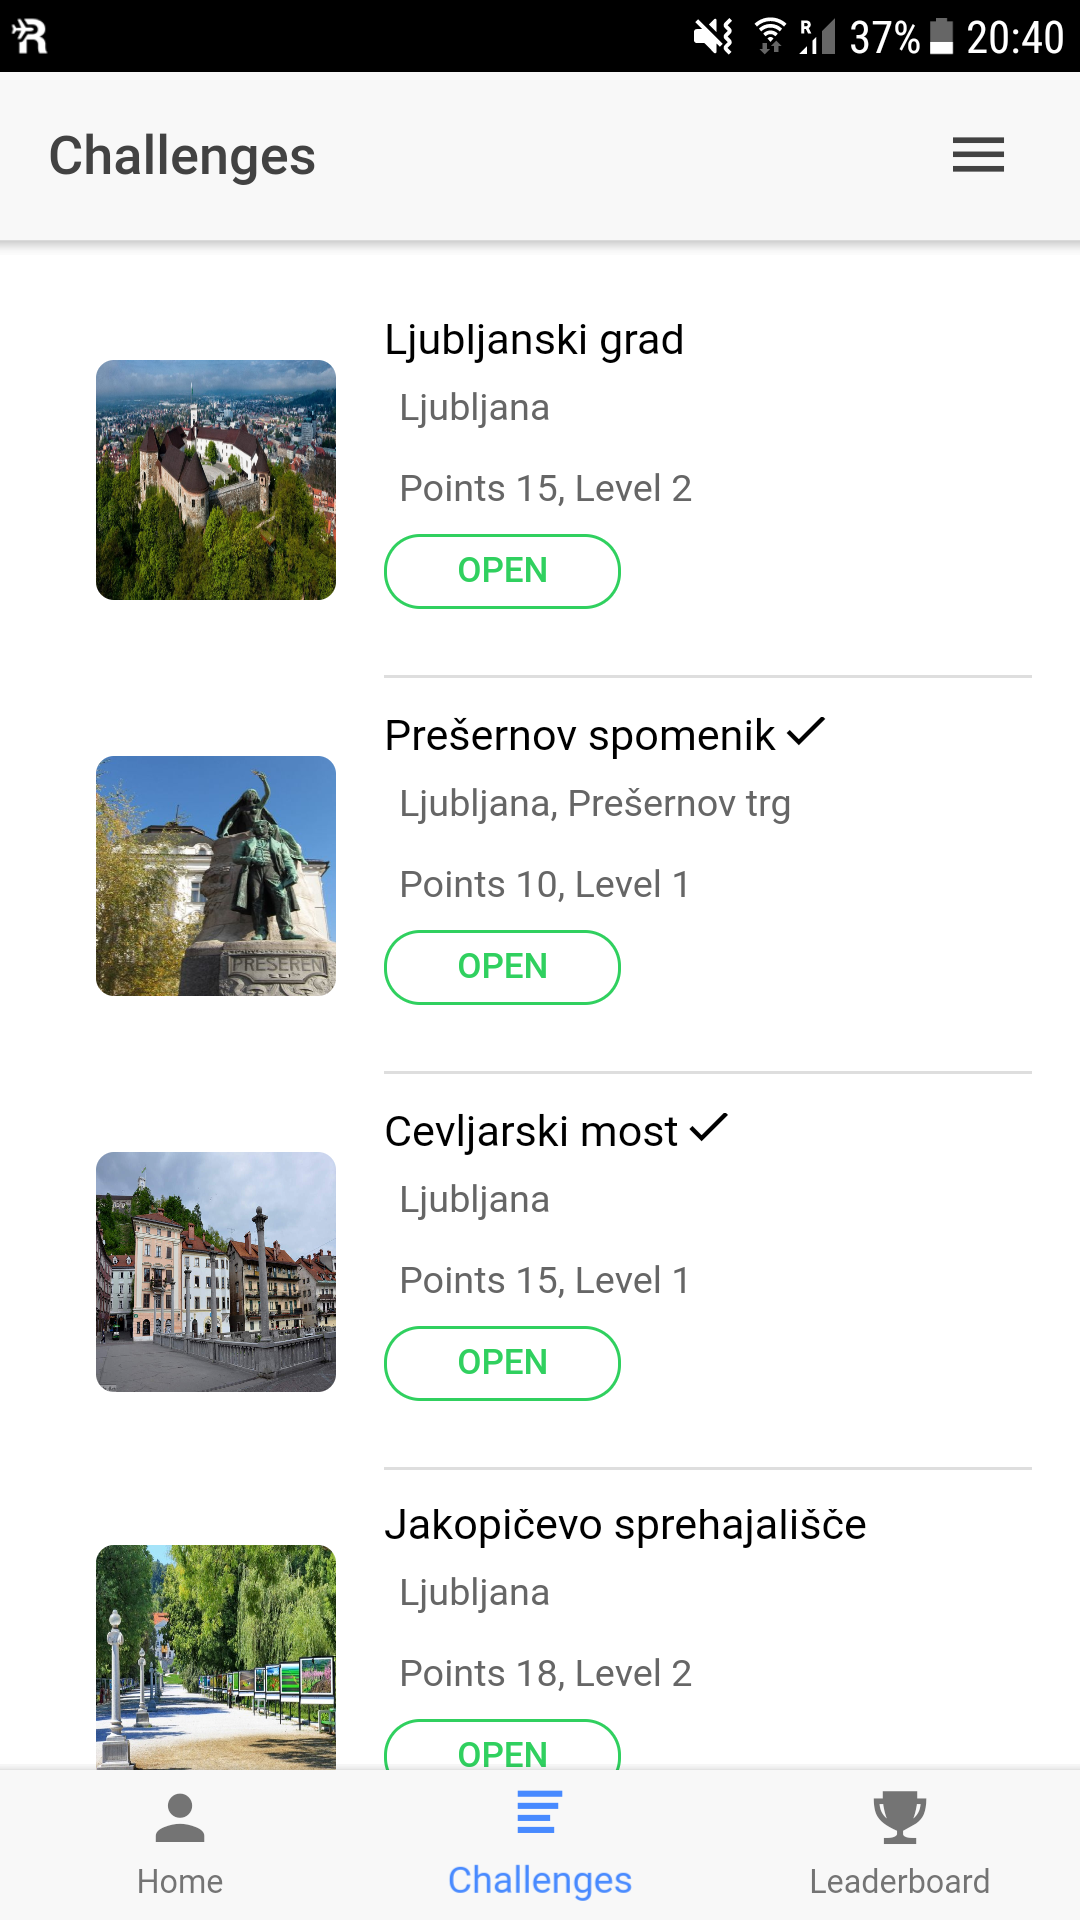
\includegraphics[height=0.8\textwidth]{slike/izzivi}
\caption{Pogled seznama izzivov.}\label{izzivi}
\end{figure}
\section{Prikaz posameznega izziva}
Kadar uporabnik izpolnjuje pogoje za ogled izziva, je na zahtevo preusmerjen na pogled, kjer ga pričaka fotografija in opis, ki sta del izziva oziroma del predmeta učenja. Vsebina opisa mora biti kratka in poučna, ter mora igralca povezati z lokacijo kjer se nahaja. Učenju tako v ozadje dodamo kontekst okolice, kar pripomore k boljši izkušnji in razumevanju učne vsebine.

Za prikaz fotografije in opisa predmeta učenja smo uporabili prednastavljeno oblikovno značko \texttt{<ion-card>}, ki obe informaciji združi v oblikovano celoto, tako da nam ni potrebno skrbeti za postavitev elementov. Za ta pogled smo uporabili spodnjo kodo.
\begin{lstlisting}
<ion-card>
    <img src="http://api.spehar.si/api/photo/{{challenge.id}}?token={{token}}">
    <ion-card-content>
        {{challenge.description}}
    </ion-card-content>
</ion-card>
\end{lstlisting}

\noindent Pod opisom prikažemo seznam vseh vprašanj in njihovih točk, na katera uporabnik lahko odgovori. Vprašanja prikažemo z zanko v izvorni kodi, podobno kot to naredimo v pogledu seznama vseh izzivov. Za oblikovanje seznama uporabljamo oblikovno značko \texttt{<ion-list>}.\\Preden je uporabnik preusmerjev v ta pogled, shranimo identifikatorje že odgovorjenih vprašanj, na katera uporabnik nato ne more odgovarjati več, zato gumb pri že odgovorjenih vprašanjih deaktiviramo in jih označimo z ikono kljukice. Vsakič preden izpišemo element v seznamu, s funkcijo \texttt{questionTaken()} preverimo ali je uporabnik na vprašanje že odgovoril pravilno.\\Sledi del kode, ki je v pogledu uporabljen za prikaz vprašanj izziva.
\begin{lstlisting}
<ion-list>
    <ion-item *ngFor="let question of questions; let i = index">
        <h2>{{question.question}} <ion-icon name="checkmark" *ngIf="questionTaken(question.id)"></ion-icon></h2>
\end{lstlisting}
Pogled posameznega izziva kot ga vidi uporabnik je prikazan na sliki~\ref{izziv}.
\begin{figure}[H]
\centering
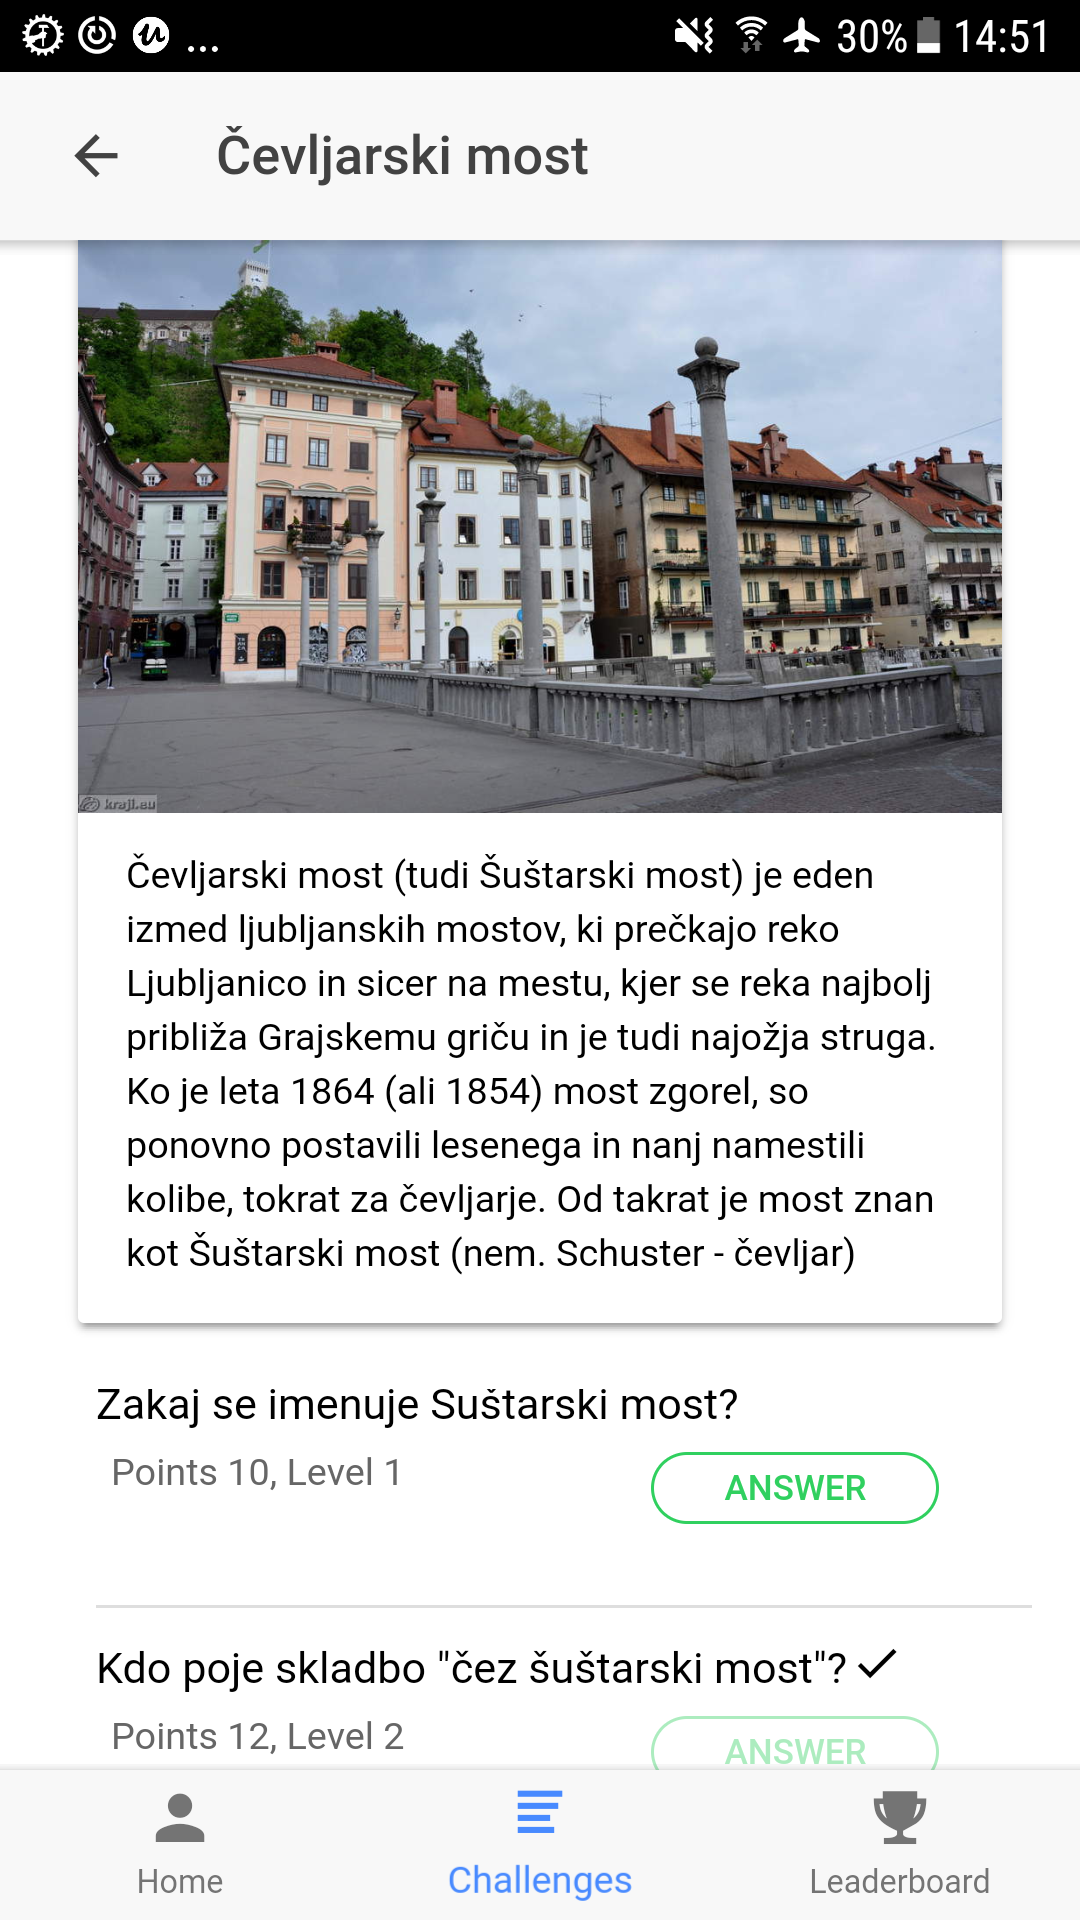
\includegraphics[height=0.8\textwidth]{slike/izziv}
\caption{Slika z opisom predmeta učenja in vprašanja.}\label{izziv}
\end{figure}
\noindent Vprašanje je označeno kot odgovorjeno, v primeru pravilnega odgovora. Tako lahko uporabnik večkrat odgovori na isto vprašanje, vendar z napačnim odgovarjanjem izgubi točke. Ob napaki se uporabniku od trenutnih točk odšteje polovica točk, namenjenih pravilnemu odgovoru. Sledi koda, ki poskrbi, da so točke uporabniku odštete, ter prikaže sporočilo v aplikaciji. 
\begin{lstlisting}
this.quService.wrongAnswer(this.question.id,localStorage.getItem('userId'),
	localStorage.getItem('token'))
    .subscribe(
    	(response) => {
            this.handleError("Wrong answer!", 'You lost ' + Math.round(this.question.points/2) + " points");
\end{lstlisting}
Slika~\ref{question} prikazuje pogled posameznega vprašanja z odgovori in gumbom za odgovor.
\begin{figure}[H]
\centering
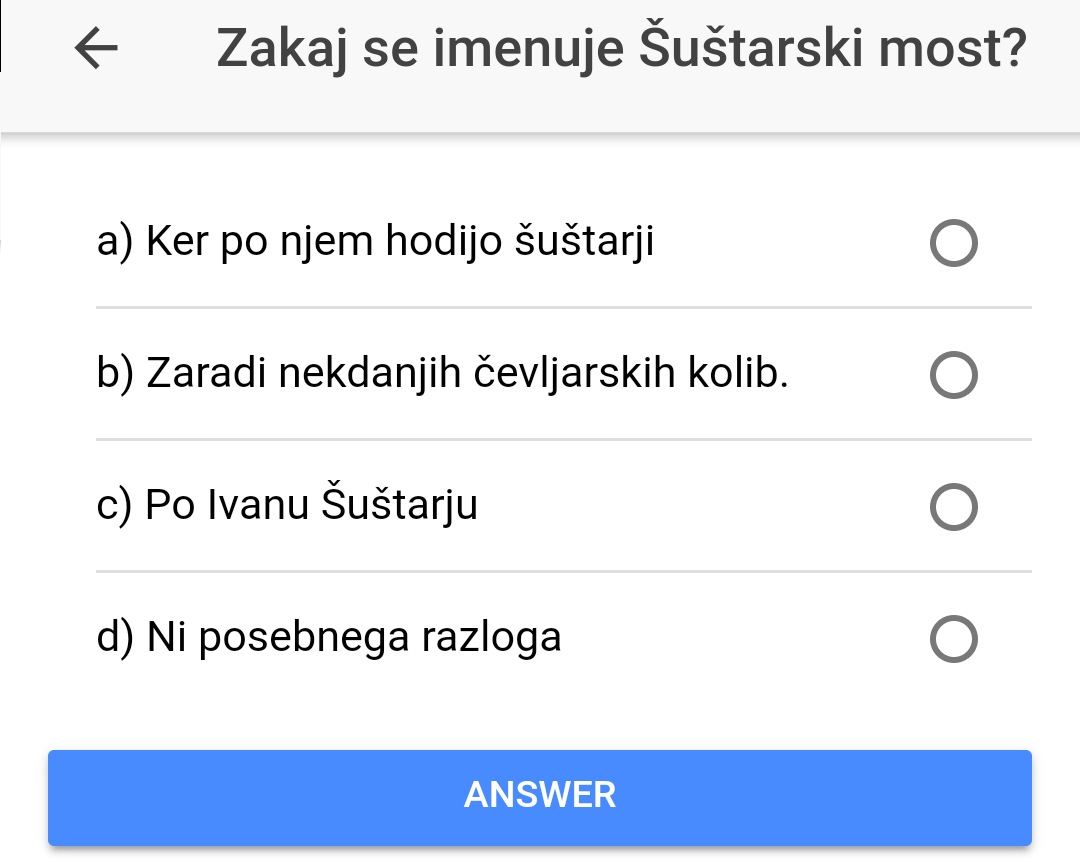
\includegraphics[height=0.5\textwidth]{slike/question}
\caption{Eno od vprašanj v izzivu.}\label{question}
\end{figure}

\section{Lestvica}
Točke, ki jih uporabniki zbirajo z obiskovanjem krajev in odgovarjanjem na vprašanja, dobijo vrednost samo, če jih lahko uporabimo za napredek v igri. Kadar želimo igralce motivirati s točkami, jim moramo napredek nekako prikazati. Pasica napredka je dober način takšnega prikaza podatkov, saj uporabnik ve koliko točk mora zbrati, da lahko preide na višji, težji nivo. Da pa uporabniki nebi tekmovali samo sami s sabo, smo razvili prikaz lestvice, kjer uporabnik vidi njegovo trenutno pozicijo med vsemi tekmovalci in se lahko primerja z najboljšimi.\\Razvili smo poseben način prikaza položaja na lestvici. Kadar je igralec uvrščen nižje od šestega mesta, pripravimo lestvico kjer mu prikažemo najboljše štiri igralce in nato igralca na mestu pred njim, ter vse ostale uporabnike za njim. S prikazom najboljših želimo dvigniti motivacijo uporabnika ter mu pokazati, da so najvišja mesta dosegljiva, obenem pa, z mestom pred njim, prikažemo najmanjši korak oziroma število točk potrebnih za napredovanje po lestvici. Spodaj je prikazan del kode, ki skrbi za ustvarjanje uporabniku prilagojene lestvice.
\begin{lstlisting}
if (position > 6) {
    for (let i = 0; i < this.leaderboard.length; i++) {
        if (i === 4) {
            this.customLeaderboard.push({position: '', points: '', username: ". . ."});
            i = position - 3;
        }
        else {
            this.customLeaderboard.push({
                id: this.leaderboard[i].id,
                position: i + 1,
                points: this.leaderboard[i].points,
                username: this.leaderboard[i].username
            })
\end{lstlisting}
\noindent V primeru, ko je uporabnik višje od šestega mesta pa izpišemo prvih deset uporabnikov po vrsti. Trenutno prijavljeni je vidno označen z zelenim ozadjem, ki je definirano v slogovnem razredu \texttt{current}. Za prikaz lestvice v uporabniškem vmesniku poskrbi naslednja koda.
\begin{lstlisting}
<ion-item *ngFor="let user of customLeaderboard"
          text-left
          [ngClass]="(user.id==userId) ? 'current' : 'normal'">
    <ion-row >
        <ion-col><h1 ion-text>{{user.position}}</h1></ion-col>
        <ion-col>
            <h1 ion-text>{{user.username}}</h1>
        </ion-col>
        <ion-col><p ion-text *ngIf="user.points!==''" text-right>{{user.points}} Points</p></ion-col>
    </ion-row>
</ion-item>
\end{lstlisting}
V izvorni kodi pogleda lestvice v zanki preverimo, če je trenutni element oziroma uporabnik, ki ga izpisujemo enak prijavljenemu uporabniku in na podlagi te informacije uporabimo pravi slogovni razred.\\Končni rezultat prikaza uporabnika na lestvici, je viden na sliki~\ref{leaderboard}.
\begin{figure}[H]
\centering
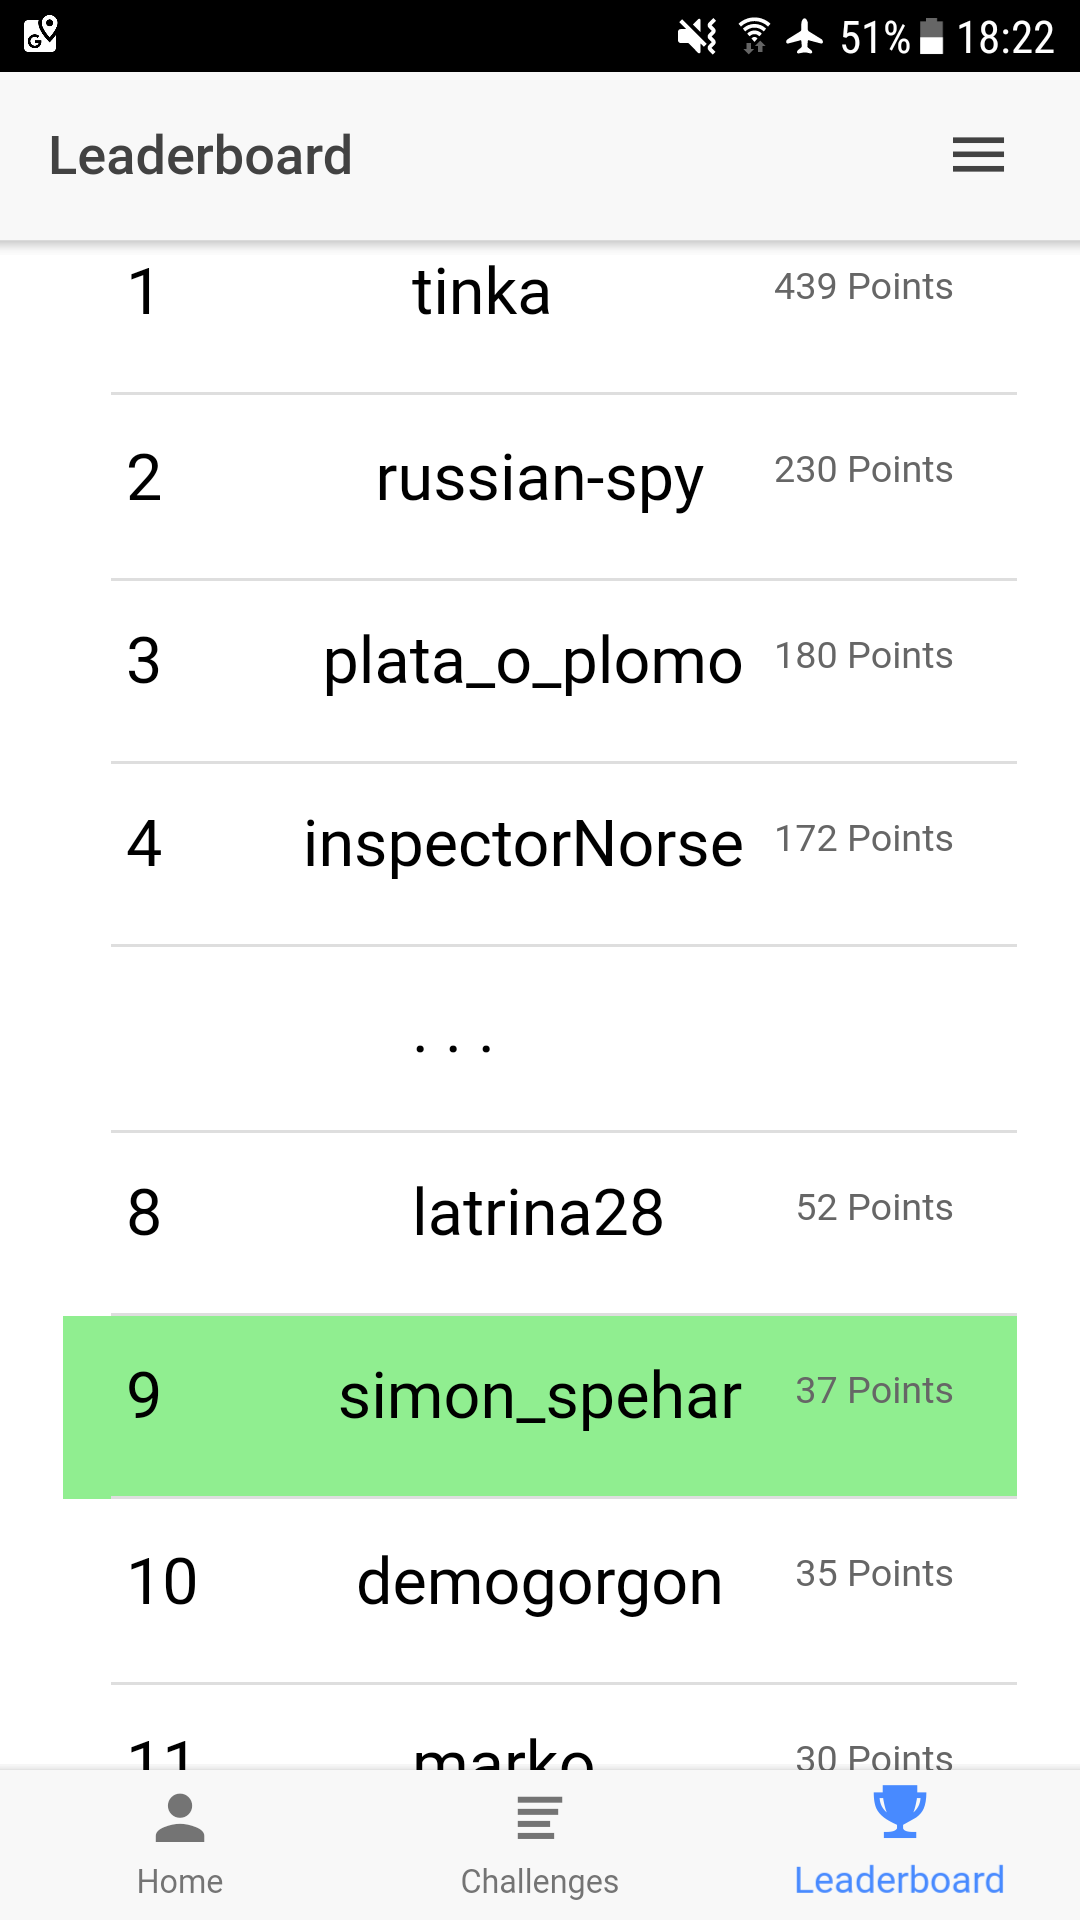
\includegraphics[height=0.9\textwidth]{slike/leaderboard}
\caption{Umestitev uporabnika na lestvico.}\label{leaderboard}
\end{figure}

\chapter{Sklep}
\label{ch8}
Učenje preko mobilnih naprav je danes pri ljudeh že ustaljena praksa. Zaradi hitrega načina življenja smo skoraj primorani v opravljanje več del hkrati. Želja po osebni rasti in učenju novih stvari je pri večini velika, vsak trenutek želimo izkoristiti za vsrkavanje novih znanj in mobilne naprave so idealen pripomoček za takšno potešitev. 

Te nam omogočajo, da smo stalno aktivni, predvsem v času, ko je večina aktivnosti onemogočenih. A to ni edina prednost mobilnosti, učenje v kontekstu z okolico nam omogoča, da digitalne informacije obogatimo z realnim svetom in jih povežemo v smiselno celoto. Zaradi tega smo se odločili, da v mobilni aplikaciji poskusimo izkoristiti uporabnikovo zavedanje okolice pri učenju ter ga celo prisilimo v obiskovanje krajev. Gamifikacija je pojem, o katerem se ne govori veliko zadnje čase, vendar to ne pomeni, da gre za prakso, ki se je ne uporablja več. Nasprotno, gamifikacija je do neke mere prisotna skoraj da v vsaki aplikaciji. Tudi, če elemente gamifikacije, kot so naprimer točke, zamenjamo z všečki, gre za podoben princip. Gre za način kako uporabnike motivirati k ponovni in večji uporabi aplikacije. V našem primeru, kjer imamo aplikacijo katere cilj je, da se uporabniki z njo učijo, smo gamifikacijo uporabili z namenom, da uporabniki odkrivajo nove vsebine in širijo svoje znanje na zabaven, tekmovalen način. V diplomskem delu smo predstavili elemente gamifikacije, ki jih lahko uporabimo pri implementaciji takšnega sistema. Takšnih elementov je še veliko in ponavadi so pri razvoju gamifikacije prisotne skupine razvijalcev ali svetovalcev, ki skrbijo za uporabniško izkušnjo. Katere elemente gamifikacije uporabiti v aplikacijah je odvisno od namena aplikacije. Sama vključitev takšnih elementov še ne zagotavlja uspeha, včasih je tudi nepotrebna. Zato potrebujemo testiranja in povratne informacije uporabnikov, ki izoblikujejo končni izdelek. To je lahko dolgotrajen postopek in se ga zato v diplomski nalogi nismo lotili, se ga pa zavedamo.\\Razvili smo sistem, ki skrbi za celoten življenjski cikel mobilnega učenja. Od ustvarjanja novih nalog preko spletne aplikacije, kasnejšega urejanja le teh, do uporabe generiranih vsebin s strani končnih uporabnikov v mobilni aplikaciji. Pri izdelavi diplomskega dela smo se naučili veliko o razvoju mobilnih aplikacij za učenje z zavedanjem okolice, o namenu gamifikacije in vpeljavi le te s stališča razvoja in obnašanja uporabnikov. 

Prostor za izboljšavo je vedno prisoten. Nismo se osredotočali na posebno temo učenja, urednik vsebine ima pri tem proste roke, kar je lahko dobro in slabo. Dizajn aplikacije ni bil naš primarni cilj. Ravili smo zadane funkcionalnosti, seveda se te lahko v prihodnosti spremenijo glede na že prej omenjena testiranja. Vsekakor pa se bomo v bodoče, ko bomo v kakšni aplikaciji za naše znanje prejeli točke, zavedali pomena in razumeli zakaj in kako takšni sistemi delujejo.

\addcontentsline{toc}{chapter}{Literatura}

\bibliographystyle{plain}
\bibliography{literatura}
\iffalse \input{edited.bbl}\fi

\end{document}

